\documentclass{article}
%Ciao!! questi sono gli appunti di Statistical Modelling For Stochastic Processes. Ho creato il pacchetto "pacco" che contiene istruzioni e pacchetti necessari per lo stile e i colori.
\usepackage{paccosmsp}
\begin{document}
\title{Statistical modelling for stochastic processes\\ spring 2024}
\author{SDS}
\date{}
\maketitle
\tableofcontents
\section{Markov Chains}
\subsection{Overview}
Let ($\Omega, \mathscr{F}, \mathbb{P}$) be a probability space. Then, a \enf{stochastic process} is a collection 
\[\{X(t,\omega), \; t\in T\}\]
of random variables
\[X:T\times\mathscr{F} \longrightarrow S\]
where:
\begin{itemize}
    \item $T$ is the \sott{index set} (typically interpreted as time); 
    \begin{example}
        $T:= \mathbb{Z}_+=\{0,1,2,\ldots\}$: $T$ is a \textit{discrete time} ($\{X_n, \; n\in\mathbb{Z}_+\}$).
    \end{example}
    \begin{example}
        $T:=\mathbb{R_+}$:$T$ is a \textit{continuous time}.
    \end{example}
    \item $S$ is the \sott{state space}. $S$ can be countable: we can take $S \subseteq \mathbb{Z}$ and denote the elements of $S$ as $i, j, k, \ldots$ or $i_1, i_2, i_3, \ldots$.
\end{itemize}
If $X_n=i$ we say that $X$ is in state $i$ or that $X$ visits $i$ at time $n$. Typically we drop the argument $\omega$ in $X(t,\omega)$ and just write $X(t)$. $X(\cdot,\omega)$ for a fixed $\omega$ is a function of $t$ and is called \sott{trajectory} of $X$.

More generally one could have:
\begin{itemize}
    \item $T \subset \mathbb{R}^d$: \textbf{random fields} (e.g. geographical coordinates: $X$ is a pair of latitude and longitude data and the state is the height data $\rightarrow T \subset \mathbb{R}^2$);
    \item $S \subset \mathbb{R}$;
    \item $S \subset \mathbb{R}^d$: \textbf{multivariate processes};
\end{itemize}

\begin{definition}
    A \enf{Markov Chain} (MC) is a discrete-time stochastic process $\{X_n,n\in\mathbb{Z}_+\}$ taking values in a countable space $S$, such that:
    \begin{align}\label{markprop}
        &\prob(X_n=i_n|X_0=i_0,\ldots,X_{n-1}=i_{n-1})\\
        =&\prob(X_n=i_n|X_{n-1}=i_{n-1})\qquad\forall n\,\geqslant1,\;\forall\,i_0,\ldots,i_n \in S.
    \end{align}
    This property is called \enf{Markov property.}
\end{definition}
Markov property defines a very broad class of Markov process es. Given the current state $X_{n-1}$, the next $X_n$ does not depend on the state previous to $n-1$. We could express these concepts in terms of $\sigma$-algebras and filtrations: if
\[
\mathscr{F}^x_n=\sigma(x_k, k\leqslant n)
\]
and 
\[
\{\mathscr{F}^x_n,n\in \mathbb{Z}_+\}
\]
is the natural filtration, the previous reads:
\[
\prob(X_n=i_n|\mathscr{F}^x_{n-1})=\prob(X_n=i_n|X_{n-1}).
\]
$\mathscr{F}^x_{n-1}$ renders useless the information previous to $n-1$.\bigskip\\
From what we studied in our earlier courses, the main assumption in classical inference was the fat that the samples were i.i.d. But at a certain point we need a more sophisticated model that gives up this assumption. If the data are not i.i.d. we need to make a choice regarding the dependence between the data. Markov processes are highly studied because they offer a way of mathematically studying the dependence between samples (another common way is recurring to \textit{Bayesian inference}). 
\begin{remark}
    The Markoviality is one way of departing from i.i.d. assumptions and all results that follow come from this property.
\end{remark}
The dyamics of $X$ are specified therefore by the right hand side of the Markov Property equation \ref{markprop}
\[p_{ij}=\prob(X_{n+1}=j|X_n=i)\]
which is called \enf{transition probability}.\\
We will assume that these are \sott{temporary homogeneous}, i.e. they do not depend on time. So we can denote
\[p_{ij}=\prob(X_{n+1}=j|X_n=i) \]
for any time $t$. We call $j$ the \textit{arrival state} ad $i$ the \textit{starting state}.
\begin{remark}
    \sott{Spatial homogeneity} is a much stronger assumption, not made here in general. In this case, $p_{ij}$ only depends on $j$: $p_{ij}=p_{0, j-1}$. For example, if we analyzed the probability of moving between the tiles of a grid, spatial homogeneity would imply that moving from one tile to another is the same regardless to the starting tile.
\end{remark}

We tipically collect the $p_{ij}$ in a \enf{transition matrix}:
\[P=(p_{ij}) \; i,j\in S\]
\begin{example}
    For $S=\{0,1,\ldots,k\}$ we have:\\
    \[\begin{bmatrix} 
    p_{00} & p_{01} & \dots & p_{0k} \\
    \vdots & \ddots&  & \vdots \\
    \vdots &  & \ddots & \vdots \\
    p_{k0} & p_{k1} & \dots & p_{kk}
\end{bmatrix}\]
\end{example}
P is a \sott{stochastic matrix} since:
\begin{itemize}
    \item $p_{ij}\geqslant 0\qquad \forall\; i,j \in S$;
    \item $\forall \;i \in S: \qquad \sum_{j\in S}p_{ij}=1$.
\end{itemize}
Now $i$ is then the conditional distribution of $X_{n+1}$ given $X_n=i$.\\
We typically use a graph to represent a MC.
\begin{example}
    \[
    P=\begin{bmatrix} 
    p_{00} & p_{01} & 0 \\
    p_{10} & 0 & p_{12} & \\
    0 & p_{21} & 0
\end{bmatrix}
    \]
    
\begin{figure}[H]
    \centering
    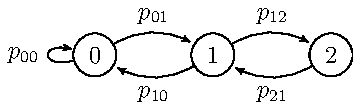
\includegraphics{standalones/pdfs/simplechain.pdf}
    \label{sonoebreo}
\end{figure}
\end{example}
Is the transition matrix enough to derive everything about the Markov process? In other words, does the transition matrix \sott{fully characterize} the distribution and the features of the process? The answer is yes but only if we include the \enf{initial distribution} of the chain.

\begin{definition}
    Define the \enf{initial distribution} of the chain
    \[
    \lambda_i=\prob(X_0=i)\qquad i\in S
    \]
    as the law of the starting state. 
\end{definition}
If \[\lambda_i=\delta_{ij}\footnote{Kronecker's delta.} =
\begin{cases}
    1,& \text{if } i=j\\
    0,              & \text{otherwise}
\end{cases}\]
then $X_0=j$ almost surely.

\begin{proposition}
    Let $X$  be a MC on $S$ countable with initial distribution $\lambda=i \in S$ and transition matrix P. Then $\lambda$ and $P$ jointly fully charcterize the law of the chain. 
\end{proposition}
\begin{proof2}
    What do we need to prove? We need to examine the joint distribution of a Markov Chain, which is an infinite sequence of random variables that are not i.i.d.: we can't therefore write the joint distribution as the product of the single distributions.

    We need to show that $(\lambda, P$) allows us to compute all joint distributions for the chain, i.e. $\forall$ choices of $0\leqslant j_1 < j_2 < \ldots < j_k$ the law $\prob(X_{j_1}=i_{j_1}, \ldots, X_{j_k}=i_{j_k})$\footnote{This is called a \sott{projection}: we are projecting an infinite sequence on a finite subset.}, which has $k$ states, can be computed with $(\lambda, P$) only. We can use the previous as the marginal of the joint distribution for times $0, \ldots, j_k$:
    \[
    \underbrace{0,1,\dots,j_{1-1}}_{\mathclap{\text{marginalize}}},\textcolor{RedViolet}{j_1},\underbrace{j_{1+1},\ldots}_{\mathclap{\text{marginalize}}},\textcolor{RedViolet}{j_2},\underbrace{\ldots}_{\mathclap{\text{marginalize}}},\textcolor{RedViolet}{j_k}
    \]
    i.e. it is
    \[
    \sum_{\underbrace{i_h\in S | h \neq j_1,\ldots,j_k}_\text{indices of times not chosen: $h \in \{o, \ldots, j_k\}$}} \prob(\underbrace{X_0=i_0, X_1=i_1,\ldots,X_{j_1}=i_{j_k}}_\text{$j_k + 1$ states})
    \]
    So it is enough to find $\prob(X_0=i_0,\ldots,X_n=i_n)$, but by the chain rule this equals to 
    \[\prob(X_0=i_0,\ldots,X_{n-1}=i_{n-1}) \cdot \prob(X_n=i_n|X_0,\ldots,X_{n-1})\]
    and thanks to Markov Property this is equal to
    \begin{align*}
           &\prob(X_0=i_0,\ldots,X_{n-1}=i_{n-1}) \cdot p_{i_{n-1},i_n}\\
           =&\ldots=\underbrace{\prob(X_0=i_0)}_{\lambda_{i_0}}\cdot       p_{i_0,i_1}\cdot\ldots\cdot p_{i_{n-1},i_n}
    \end{align*}
    So we only need $\lambda_{i_0}$ and the $P$ matrix.
\end{proof2}

We can use a compact notation (took from Norris textbook)
\[X \sim \text{Markov}(\lambda,P).\]

\begin{definition}
  We define the \enf{$k$-step transition probabilities} as
\begin{align*}
    &p_{ij}^{(k)} := \prob(X_{n+k}=j|X_n=i), \qquad k \in \mathbb{N}\\
    &p_{ij}^{(0)} := \delta_{ij} = \begin{cases}
        1 & i=j\\
        0 & \text{else}
    \end{cases}
\end{align*}
\end{definition}

\begin{proposition}{\enf{Chapman-Kolmogorov equations:}}
    for all $e$, $m \in \mathbb{Z}_+$
    \begin{equation}\label{chapkolm}
        p_{ij}^{(e+m}=\sum_{k<j}p_{ik}^{(e)}\cdot p_{kj}^{(m)}
    \end{equation}
\end{proposition}
The proof is left as exercise (use graphical intuition below: marginalize out unwanted states and use Markov property). 
\begin{figure}[H]
    \centering
 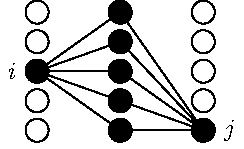
\includegraphics{standalones/pdfs/marginchain}
    \label{mc graph} %porcoddio sono un cazzo di dragooOOO
\end{figure}

If you take the transition matrix to the power of $k$, $P^k$ is still a stochastic matrix and the entries are $p_{ij}^(k)$.
\begin{example}
    \begin{figure}[H]
    \centering
    \begin{tikzpicture}[->,>=stealth',shorten >=2pt, line width=0.5pt, node distance=2cm]
        \node [circle, draw] (zero) {0};
        \node [circle, draw] (one) [right of=zero] {1};
        \path (zero) edge [bend left] node [above] {$\alpha$} (one);
        \path (zero) edge [loop left] node [left] {$1-\alpha$} (zero);
        \path (one) edge [loop right] node [right] {$1-\beta$} (zero);
        \path (one) edge [bend left] node [below] {$\beta$} (zero);
    \end{tikzpicture}
    \label{sadasdasf}
\end{figure}
\[
P^2=P\cdot P=\ldots=\begin{bmatrix}
    p_{00}^{(2)} & p_{01}^{(2)}\\
    p_{10}^{(2)} & p_{11}^{(2)}
\end{bmatrix}
\]
In this case, the intermediate states don't matter. For instance we have $p_{00}^{(2)}=p_{00}p_{00}+p_{01}p_{10}$
\end{example}
\subsection{Notable Markov processes}
\subsubsection*{Random Walk}
Given $X_0$, the simple random walk is defined as
\[X_n=X_{n-1}+Y_n\]
$Y_n$s are i.i.d.:
\[
Y_n=\begin{cases}
    1 &\text{with probability}\; p\\
    -1 &\text{with probability}\; 1-p
\end{cases}
\]
\[
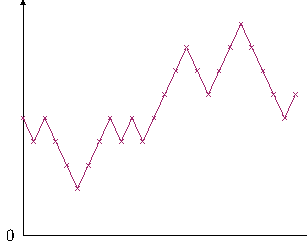
\includegraphics{standalones/pdfs/simplerw}
\]
if $p=\frac{1}{2}$ the the random walk is \sott{symmetric}.\\
Random walks have application, for instance, in:
\begin{itemize}
    \item approximation of Brownian motion and other diffusion processes useful in:
    \begin{itemize}
        \item physics;
        \item math finance;
        \item math biology;
    \end{itemize}
    \item random explorations of space:
    \begin{itemize}
        \item Monte-Carlo integration (Monte-Carlo Markov Chain methods);
        \item stochastic optimization
        \item integral approximation
    \end{itemize}
\end{itemize}
Some possible extensions are:
\begin{itemize}
    \item changing the state space dimension: imagine a symmetric random walk in $\mathbb{Z}^d$, $i,j \in \mathbb{Z}^d$ with $i=(i_1,\ldots,i_d)$:
    \[
    p_{ij}=\begin{cases}
        \frac{1}{2d} & \text{if}\quad \sum_{k=1}^q|i_k-j_k|=1\\
        0 & \text{else;}
    \end{cases}
    \]
    \item change law of $Y_n:\prob(Y_n=1)=a_i, \; \in \mathbb{Z}$ (the case of the distribution being heavy tailed is particularly interesting);
    \item change the topology of $S$:
    \begin{itemize}
        \item Random walk on manifold sphere, on torus...;
        \item Random walk on graphs; for example choose uniformly with probability $q$ a node in the graph (Google PageRank Algorithm).
    \end{itemize}
\end{itemize}
\subsubsection*{Birth-and-death chains}
We define the transition probabilities as
\[
p_{ij}=\begin{cases}
    p_i & j=i+1\\
    1-p_i & j=(i-1)^+\\
    0 &\text{else}
\end{cases}
\]
\begin{figure}[H]
    \centering
    \begin{tikzpicture}[->,>=stealth',shorten >=2pt, line width=0.5pt, node distance=2cm]
        \node [circle, draw] (zero) {0};
        \node [circle, draw] (one) [right of=zero] {1};
        \node [circle, draw] (two) [right of= one] {2};
        \node [circle, draw] (dots) [right of=two] {$\ldots$};
        \path (zero) edge [bend left] node [above] {$p_0$} (one);
        \path (zero) edge [loop left] node [left] {$1-p_0$} (zero);
        \path (one) edge [bend left] node [below] {$1-p_1$} (zero);
        \path (one) edge [bend left] node [above] {$p_1$} (two);
        \path (two) edge [bend left] node [above] {$p_2$} (dots);
        \path (dots) edge [bend left] node [below] {} (two);
        \path (two) edge [bend left] node [below] {$1-p_2$} (one);
    \end{tikzpicture}
    \label{ahah}
\end{figure}
\begin{itemize}
    \item Time-varying size of a population (animal, viruses, numbero of request to a CPU...)
    \item size of a queue at a server
    \item dimension of a multivariate distribution used for estimation
    \item dimension $k$ of a mixture model
    \[
    \text{i.e.} \qquad \sum_{i=k}^k w_i f_i
    \]
    with $\sum_{w_i}=1$ and $f_i$ being a density.
\end{itemize}
\subsubsection*{Pòlya urns}
An urn contains $W_0$ white balls and $B_0$ black a ball. We draw a ball, check its colour, put it back and add to the urn another ball of the same colour: this behaviour is called \sott{reinforcement} and it is the opposite of drawing without placement. Let $W_n$ be the number of white balls after n draws (steps):
\[
\prob(W_{n+1}=j|W_0,\ldots,W_n)=\begin{cases}
    \frac{W_n}{Wn+Bn}\rightarrow\text{"draw white"} &j=W_n+1\rightarrow\text{"add white"}\\
    \frac{B_n}{Wn+Bn}\rightarrow\text{"draw black"} &j=W_n\rightarrow\text{"same number of whites"}\\
    0 & \text{else}
\end{cases}
\]
\begin{align*}
    W_n+&B_n=W_0+B_{0+n}\\
    &B_n=W_0+B_{0+n}-W_n
\end{align*}
The probability only depends on $W_n$ and the previous $W$s are irrelevant, so the process is a Markov Chain
These are applied in Bayesian inference, since they generate \sott{exchangeable sequences} ($(X_1, X_2)\stackrel{d}{=}(X_2,X_1)$). A classical result which is often used is:
\[
\frac{W_n}{W_n+B_n}\xrightarrow{a.s}\theta\sim Beta(W_0, B_0)
\]
\subsubsection*{Branching Processes}
Branching processes are a simple model for evolving populations with reproduction. The basic formulation (Galton-Watson) is:
\begin{itemize}
    \item individuals live on period;
    \item individuals generate clones independently (the original motivation was the survival of family names);
    \item the next generation is formed by the offspring of the previous generation.
\end{itemize}

\begin{figure}[H]
    \centering
    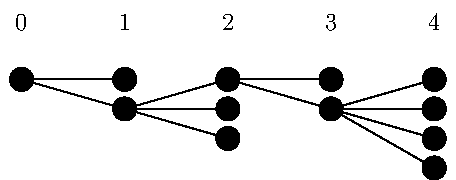
\includegraphics{standalones/pdfs/bp}
    \label{generatons}
\end{figure}
Useful applications:
\begin{itemize}
    \item epidemiology (virus contagion);
    \item population genetics;
    \item physics (random number of neutron produced at collisions).
\end{itemize}
Interesting extensions:
\begin{itemize}
    \item extend to $k$ types;
    \item add immigration.
\end{itemize}
Let $X_n$ be the number of individuals in generation $n$ and $Y_i$ be the number of clones/offspring of individual $i$. We have $Y_i \stackrel{i.i.d.}{\sim} p_Y$ on $\mathbb{Z}_+$.
\[
X_n=Y_1+Y_2+\ldots+Y_{X_{n-1}}=\sum_{i=1}^{X_{n-1}}Y_i\independent X_{n-2},X_{n-3},\ldots
\]
So the process is a Markov chain. 

\begin{proposition}{\enf{Branching Property:}}
    Denote by $X^{(i)}=\{{X_n}, n \in \mathbb{Z}_+|X_0=1\}$, characterizing the chain by a fixed starting point, the branching process started at $i$. Let $\Tilde{X},\hat{X}$ be independent copies of $X$. Then
    \begin{equation}
        X^{(i+j)}\stackrel{d}{=}\Tilde{X}^{(i)}+\hat{X}^{(j)}
    \end{equation}
    This is called \enf{branching property}.
\end{proposition}
\begin{proof2}
    Let 
    \[
    g_{z}(s)=\ev{e^{sZ}}
    \]
    be the moment generating function of $Z$. We are interested in the moment generating function of $X_1|X_0=i$.
    \begin{align*}
       g_{X_1^{(i)}}=g_{\sum_{j=1}^{i}Y_j} =(g_Y)^i
    \end{align*} 
    This moment generating function characterizes the one step transition probability of getting to $X_1$, that is the population size at $n=1$, from the state $X_0=i$. Now
    \begin{align*}
         &g_{\{\Tilde{X}_1^{(i)}+\hat{X}_1^{(j)}\}}=g_{\Tilde{X}_1^{(i)}}\cdot g_{\hat{X}_1^{(j)}}=\\
         =(&g_Y)^i\cdot(g_Y)^j=(g_Y)^{i+j}=g_{X_1^{(i+j)}}
    \end{align*}
    We have now proved for one step that, since $\Tilde{X}_1^{(i)}+\hat{X}_1^{(j)}$ and $X_1^{(i+j)}$ share the same moment generating function, they have the same distribution. To extend this result to every step we can use Markov property, so that $X^{(i+j)}_1\stackrel{d}{=}\Tilde{X}^{(i)}_1+\hat{X}^{(j)}_1$ characterizes the law of the entire chain.
\end{proof2}
An interesting extension of the model consists in the behaviour of a population during extinction. This ultimately depends on:
\[
\ev{Y}=\begin{cases}
    <1 & X\; \text{is subcritical}\\
    =1 & X\; \text{is critical}\\
    >1 & X\; \text{is supercritical}\\
\end{cases}
\]
An interesting case is given by introducing immigration to the subcritical case. This is called \enf{Galton-Watson} branching process.
\subsubsection*{Wright-Fisher models}
These model the time-varying frequency of 2 types (in general k or $\infty$ many types) in an evolving population of constant size. The original motivation was modelling the allelic type frequency of a gene locus. These models have the following characteristics:
\begin{itemize}
    \item individuals live 1 period;
    \item individuals can be of type 0 or 1;
    \item population size is $N$ $\forall n \geqslant \mathbb{Z}_+$;
\end{itemize}

\begin{figure}[H]
    \centering
    \begin{tikzpicture}[-,>=stealth', line width=0.5pt, node distance=0.5cm]
        \node [circle] (zero) {0};
        \node [circle, draw, shade, shading=ball, circle, ball color=RedViolet!80!white] (a) [below=0.4cm of zero]{};
        \node [circle, draw, shade, shading=ball, circle, ball color=RedViolet!80!white] (b) [below of= a]{};
        \node [circle, draw, shade, shading=ball, circle, ball color=RedViolet!80!white] (c) [below of= b]{};
        \node [circle, draw, shade,shading=ball,circle,ball color=Dandelion!80!white] (d) [below of= c]{};
        
        \node [circle] (one)[right=1cm of zero] {1};
        \node [circle, draw, shade, shading=ball, circle, ball color=RedViolet!80!white] (e) [below=0.4cm of one]{};
        \node [circle, draw, shade, shading=ball, circle, ball color=RedViolet!80!white] (f) [below of= e]{};
        \node [circle, draw, shade,shading=ball,circle,ball color=Dandelion!80!white] (g) [below of= f]{};
        \node [circle, draw, shade,shading=ball,circle,ball color=Dandelion!80!white] (h) [below of= g]{};
        
        \node [circle] (two)[right=1cm of one] {2};
        \node [circle, draw, shade, shading=ball, circle, ball color=RedViolet!80!white] (i) [below=0.4cm of two]{};
        \node [circle, draw, shade, shading=ball, circle, ball color=RedViolet!80!white] (j) [below of= i]{};
        \node [circle, draw, shade, shading=ball, circle, ball color=RedViolet!80!white] (k) [below of= j]{};
        \node [circle, draw, shade,shading=ball,circle,ball color=Dandelion!80!white] (l) [below of= k]{};        
        \node [circle] (three)[right=1cm of two] {3};
        \node [circle, draw, shade, shading=ball, circle, ball color=RedViolet!80!white] (m) [below=0.4cm of three]{};
        \node [circle, draw, shade,shading=ball,circle,ball color=Dandelion!80!white] (n) [below of= m]{};
        \node [circle, draw, shade,shading=ball,circle,ball color=Dandelion!80!white] (o) [below of= n]{};
        \node [circle, draw, shade,shading=ball,circle,ball color=Dandelion!80!white] (p) [below of= o]{};

        \path (a) edge node [below] {} (e);
        \path (a) edge node [below] {} (f);
        \path (d) edge node [below] {} (g); 
        \path (d) edge node [below] {} (h); 

        \path (e) edge node [below] {} (i); 
        \path (e) edge node [below] {} (j); 
        \path (e) edge node [below] {} (k); 
        \path (h) edge node [below] {} (l); 

        \path (j) edge node [below] {} (m); 
        \path (l) edge node [below] {} (n); 
        \path (l) edge node [below] {} (o); 
        \path (l) edge node [below] {} (p); 
    \end{tikzpicture}
    \label{wright models}
\end{figure}
We have now constrained the population size, so each parent can generate from 0 to $N$ offspring and therefore birth events are no longer independent. A useful approach to model this behaviour is to imagine that during next generation individuals choose their parent at random from the previous generation, with the condition that it must be of the same type.\\
Let $X_n$ be the number of type-0 individuals at time $n$. The individuals at generation $n$ are:
\begin{itemize}
    \item of type-0 with probability $\frac{X_n}{N}$;
    \item of type-1 with probability $1-\frac{X_n}{N}$;
\end{itemize}
So every member of a generation chooses its parent by a Bernoulli trial \sott{independently}. Since we have $N$ Bernoulli trial with parameter $p=\frac{X_n}{N}$, we have that:
\[
X_n|X_{n-1}\sim Binom(N,\frac{X_{n-1}}{N}).
\]
Note that 
\begin{align*}
    \text{if}\quad &X_{n-1}=0 \implies X_n=0\qquad\text{a.s}\\
    \text{if}\quad &X_{n-1}=N \implies X_n=N\qquad\text{a.s}.
\end{align*}

\begin{figure}[H]
    \centering
        \begin{tikzpicture}
            \begin{axis}[
                xlabel=0,
                every axis x label/.style={
                at={(ticklabel* cs:-0.01)},
                anchor=east,
            },
                ylabel=\empty,
                xmin=0, xmax=52,
                ymin=0, ymax=100,
                axis y line=left,
                y axis line style={opacity=0},
                ytick=\empty,
                xtick={46}, 
                xtick style={draw=black}, 
                xticklabel={fixation event}, 
                axis x line*=bottom
                        ]
                \addplot[mark=x,RedViolet] plot coordinates {
                    (0,50)
                    (2,40)
                    (4,50)
                    (6,40)
                    (8,30)
                    (10,20)
                    (12,30)
                    (14,40)
                    (16,50)
                    (18,40)
                    (20,50)
                    (22,40)
                    (24,30)
                    (26,20)
                    (28,30)
                    (30,40)
                    (32,30)
                    (34,20)
                    (36,10)
                    (38,20)
                    (40,10)
                    (42,20)
                    (44,10)
                    (46,0)
                    (48,0)
                    (50,0)
                };
                %\node[below,RedViolet,align=left] at (46,-0.08) {\footnotesize fixation event};
            \end{axis}
                \begin{axis}[
                xlabel=$N$,
                    every axis x label/.style={
                at={(ticklabel* cs:-0.01)},
                anchor=east,
            },
                ylabel=\empty,
                xmin=0, xmax=30,
                ymin=0, ymax=100,
                axis y line=left,
                y axis line style={opacity=0},
                ytick=\empty,
                xtick=\empty,
                axis x line*=top]
            \end{axis}
    \end{tikzpicture}
    \label{camminata}
\end{figure}
Some useful extension may include:
\begin{itemize}
    \item mutations;
    \item $k\leqslant\infty$ types;
    \item uncountably many types.
\end{itemize}
For example, set mutations such that they only occur to the other type:
\[
\alpha=\prob(1\rightarrow0)\qquad\beta=\prob(0\rightarrow1).
\]
Mutations take place before reproduction (that is, before the binomial resampling method). We have:
\begin{itemize}
    \item a $Bernoulli(\beta)$ trial on each of $i$ individual of type 0. On average:
    \begin{itemize}
        \item $i\beta$ individuals become of type 1;
        \item $i(1-\beta)$ individuals remain of type 0;
    \end{itemize}
    \item a $Bernoulli(\alpha)$ trial on each of $N-i$ individual of type 1. On average:
    \begin{itemize}
        \item $(N-i)\alpha$ individuals become of type 0;
        \item $(N-i)(1-\alpha)$ individuals remain of type 1.
    \end{itemize}
\end{itemize}
After mutation, the expected proportions are:
\begin{alignat*}{3}
    &\text{type 0:}&&\qquad \Tilde{p_i}&&=\frac{1}{N}(i(1-\beta)+(N-i)\alpha)=\\
    & && &&=\frac{i}{N}(1-\beta)+(N-i)\alpha=\\
    & && &&=p_i(1-\beta)+(1-p_i)\alpha.\\
    \\
    &\text{type 1:}\qquad &&1-\tilde{p_i}&&=p_i\beta+(1-p_i)(1-\alpha).
\end{alignat*}
We can interpret $\tilde{p}_i$ as the \sott{percentage} of type 0 individuals (in expectation) before resampling. The transition probability has become:
\[=0
p_{ij}=\prob(X_{n+1}=j|X_n=i)=\binom{N}{j}\Tilde{p}_i^j(i-\Tilde{p}_i)^{N-j}
\]
Now, if $i=0\implies p_i=\frac{i}{N}=0\implies\Tilde{p}_i=\alpha\implies\prob(X_{n+1}>0|X_n=0)=1-(1-\alpha)^N>0$.\\
If $X_n$ is at the boundary $X_n \in \{o,N\}$, now there is positive probability of going back to the interior of the space state.
\subsubsection*{Transformation of Branching Processes}
Intuitively, there are two branching processes embedded in the Wright-Fisher trajectory. We can formalize this connection:

\begin{proposition}
    Let $X$ and $W$ be two independent branching processes with the same Poisson offspring distribution. Then, conditional on the total population size being constant and equal to $N$, $X$ and $W=N-X$ are Wright-Fisher chains.
\end{proposition}
\begin{proof2}
    \begin{align*}
        X_n&=\text{n° of type 0 individuals}\\
        W_n&=\text{n° of type 1 individuals}\\
    \end{align*}
    With per capita offspring
    \[
    Y\sim Pois(\lambda_j) \qquad j=0,1
    \]
    where $j$ is specific to the first and to the second branching process. Now, since the sum of Poisson variables is still a Poisson variable,
    \begin{align*}
        X_n &= \sum_{i=1}^{X_{n-1}}Y_i \sim Pois(X_{n-1}\lambda_0)\\
        W_n &= \sum_{i=1}^{W_{n-1}}Y_i \sim Pois(W_{n-1}\lambda_1)\\
    \end{align*}
    We know, in general, that
    \[
    Z_j\sim Pois(\gamma_j),\;j=0,1 \implies Z_0|Z_0+Z_1=N\sim Binom\biggl(N,\frac{\gamma_0}{\gamma_0+\gamma_1}\biggr)
    \]
    Let's apply this property:
    \[
    X_n|X_n+W_n=N,X_{n-1},W_{n-1}\sim Binom(N,q_{n-1})
    \]
    What we expect is for the parameter $q_{n-1}$ to only depend on state $n-1$. We know that:
    \[
    q_{n-1}=\frac{X_{n-1}\lambda_0}{X_{n-1}\lambda_0+\underbrace{W_{n-1}}_{\mathclap{N-X_{n-1}\;\text{because we are conditioning on the whole population}}}\lambda_1}=\frac{X_{n-1}\lambda_0}{X_{n-1}(\lambda_0-\lambda_1)+N\lambda_1}
    \]
    But we said that the offspring distribution is the \textit{same} Poisson distribution: so
    \begin{align*}
        &\lambda_0=\lambda_1\implies q_{n-1}=\frac{X_{n-1}}{N}\\
        \implies &X_n|X_{N-1},X_n+W_n=N \sim Binom\biggl(N,\frac{X_{n-1}}{N}\biggr)
    \end{align*}
    which is the transition probability of the Wright-Fisher chains, which characterizes the law of the entire chain. We are therefore claiming that the random variables whose state space is the $\infty$ trajectories of the chain is governed by one law.
\end{proof2}
\subsection{Review of Markov Property}
The property we gave that the beginning can be seen as a regeneration property:
\[
X\sim Markov(\lambda,P) \implies \{X_{n+k},k\geqslant 0|X_n=i\}\sim Markov(\delta_i,P).
\] 
Here $n$ is fixed and from $n$ onward the chain starts afresh with the same properties. What if $n$ is a random variable $T$, indicating a random time?

\begin{definition}{\enf{strong Markov property:}}
    We are interested in establishing the \enf{strong Markov property}:
    \begin{equation}
        \prob(X_{T+1}=j|X_0,\ldots,X_T=i)=\prob(X_{T+1}=j|X_T=i)
    \end{equation}
\end{definition}
Not all random times are suitable: let $\{\mathscr{F}\}_{n\geqslant 0}$ be the \sott{natural filtration} generated by $X$, where $\mathscr{F}_n=\sigma(X_u, 0\leqslant u \leqslant n)$ which is interpreted as the \textit{flow of information} generated by the $X$ trajectory up to time $n$.\\ A random variable $T:\Omega\rightarrow\mathbb{N}\cup\{\infty\}$ is a \enf{stopping time} for $X$ if 
\[
\{\omega\in\Omega :T(\omega)=n\in\mathscr{F}_n\}
\]
i.e. $\{T=n\}$ is $\mathscr{F}_n$-measurable: we can express $\{T=n\}$ in terms of $X_0,X_1,\ldots,X_n$. If we are interested in other relations:
\[
    \{T=n\}\in\mathscr{F}_n\implies\begin{cases}
        \{T\leqslant n\}=\bigcup_{i \leqslant n}\{T=n\}\in\mathscr{F}_n\\
        \{T\neq n\}=\{T=n\}^c\in\mathscr{F}_n\\
        \ldots
    \end{cases}
\]

\begin{example}{\enf{First passage time/first visit to $i$}:}
    \[
    T=\inf\{n\geqslant 1: X_n=i\}.
    \]
    Is $T$ a stopping time? The event $\{T=n\}=\{X_0 \neq i, X_1 \neq i, \ldots, X_{n-1}\neq i, X_n=i\}$ by definition belongs to $\mathscr{F}_n$, so it is a stopping time.
\end{example}
\begin{example}{\enf{Last exit time from $\mathbf{A \subset S}$}}
    \[
    T=\sup\{n\geqslant 0: X_n\in A\}.
    \]
    Is $T$ a stopping time? The event depends on $\{X_{n+m},m\geqslant 1\}$. $\{T=m\}$ does not belong to $\mathscr{F}_n$ because it is anticipating using future information: $T$ is \sott{not} a stopping time.
\end{example}

\begin{theorem}{\enf{Strong Markov Property:}}
    Let $X\sim Markov(\lambda,P)$ and $T$ be a stopping time for $X$. Then, conditional on $T<\infty$ and $X_T=i$, 
    \[
    \{X_{T+n},n\geqslant 0\}\sim Markov(\delta_i,P)
    \]
    is \textbf{independent} on the chain before time $T$.
\end{theorem}
If $T$ is a stopping time (meaning that it depends on the past only) the the chain \sott{regenerates} from $T$ with the same properties.
\begin{example}
    Let $T$ be the first visit to $j$ and $T'=T-1$ the time prior to entering j for the 1st time. $\{T'=n\}$ depends on $X_{n+1}$ which implies that $\{T'=n\}\notin\mathscr{F}_n$. Conditional to $X_{T'}=i$ the process is not Markov:
    \[
    \{X_{T'+n},n\geqslant 0\}\not\sim Markov(\delta_i,P)
    \]
    Why? The problem is that if $n=1$ then the first step of the chain is \sott{deterministic}, since we are imposing it to be $j$ instead of following the transition matrix:
    \[
    \prob(X_{T'+1}=j|X_{T'}=i)=1\neq p_{ij} \qquad\text{since}\quad X_T=X_{T'+1}=j
    \]
    so the chain does not start afresh with the same distribution properties.
\end{example}
\begin{example}
    Suppose we observe $X$ only when $X_n\in A\subset S$ (for instance, imagine we have an instrument only capable of measuring above a certain threshold $A$). $T^{(m)}=inf\{n> T^{(m)}:X_n \in A\}$ is the time of the $n$-th visit to $A$ and $Y_m:=X_{T^{(m)}}$.\\
    Assume $\prob(T^{(m)}<\infty)=1 \quad \forall m \geqslant 1$:
    \begin{align*}
        &\prob(Y_{m+1}=i_{m+1}|Y_1=i_1,\ldots,Y_m=i_m)=\\
        =&\prob(X_{T^{(m+1)}}=i_{m+1}|X_{T^{(1)}}=i_1,\ldots,X_{T^{(m)}}=i_m)=\\
        &\text{\small(by strong Markov property)}\\
        =&\prob(X_{T^{(m+1)}}=i_{m+1}|X_{T^{(m)}}=i_m)
    \end{align*}
    which means that $Y$ is a Markov Chain on $A$. If I have a Markov chain only observable on a subset then I can "skip" intermediate steps and still have a Markov chain. This is pretty cool.
\end{example}
\subsection{Properties of Markov chains}
The goal of this section is to find the conditions on $P$ to claim certain properties of Markov Chains, especially concerning long-run behaviour.

\subsubsection{Communication classes}
\begin{definition}
    A state is \enf{accessible} from $i$ if $p_{ij}^{(n)}>0$ for some $n$. Two states reciprocally accessible are said to \enf{communicate}.
\end{definition}
If a state is accessible from another state it means that the chain can go there in a finite number of steps.
\begin{example}
    \begin{minipage}{0.5\textwidth}
        \begin{figure}[H]
            \centering
            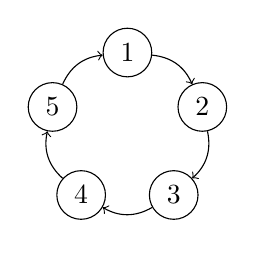
\begin{tikzpicture}[->]
                \foreach \i [count=\j from 1] in {90,18,...,-198} \node[circle,draw] (\j) at (\i:1) {\j};
                \path (1) edge [bend left] node [below] {} (2);
                \path (2) edge [bend left] node [below] {} (3);
                \path (3) edge [bend left] node [below] {} (4);
                \path (4) edge [bend left] node [below] {} (5);
                \path (5) edge [bend left] node [below] {} (1);
            \end{tikzpicture}
        \end{figure}
    \end{minipage} \hfill
    \begin{minipage}{0.45\textwidth}
    In this case all the states communicate, since it is possible to go from one to any other with at most 5$<\infty$ steps. 
    \end{minipage}
\end{example}
Communicating states form an \enf{equivalence class}: the relation is reflective, symmetric and transitive. This can be proved using the Chapman-Kolmogorov equation (Eq. \ref{chapkolm}). $S$ can be split in two or more classes of communicating states, thus obtaining a \textbf{macroscopic description} of the chain dynamics.
\begin{example}\label{irr}
\[
    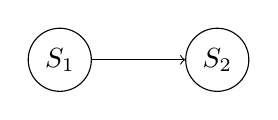
\begin{tikzpicture}[node distance=2cm]
        \node[circle,draw](2){$S_2$};
        \node[circle, draw](1)[left of=2]{$S_1$} edge[->] (2);
    \end{tikzpicture}
    \qquad S_1, S_2 \subset S
\]
In this case, once the chain leaves $S_1$ it can't go back. $S_2$ can be accessed by $S_1$ but not vice-versa. On the long run we can say that we should focus on $S_2$, since $S_1$ will be left for good sooner or later.
\end{example}

\subsubsection{Irreducibility
}
\begin{definition}
    A Markov chain with a single equivalence class generated by communicating states is said to be \enf{irreducible}.
\end{definition}
For instance, in the previous example the chain is not irreducible but once the chain leaves $S_1$ it becomes irreducible in $S_2$.\\
What about the main Markov processes?
\begin{itemize}
    \item The simple random walk is \sott{irreducible}: we can always go in every state;
    \item in branching processes, if $X_n=0$ then the process stops and $X_{n+1}=0$. This means that $\{1,2,\ldots\}$ are not accessible from 0 and the chain is therefore \sott{not irreducible};
    \item in Wright-Fisher process with no mutations we face a similar situation: $X_n=0\implies X_{n+1}=0 $ and $X_n=N\implies X_{n+1}=N $: $\{1,\ldots,N-1\}$ are not accessible from $\{0,N\}$ and the chain is therefore \sott{not irreducible}. The introduction of mutations, though, would make it irreducible.
\end{itemize}

\subsubsection{Periodicity}
\begin{definition}
    We define the \enf{period} $d(i)$ of $i\in S$ the greatest common divisor of all $n\geqslant 1$ such that $p_{ii}^{(n)}>0$. If $p_{ii}^{(n)}>0$ for all sufficiently large $n$ (or if $d(i)=1$) we say that $i$ is \enf{aperiodic}.
\end{definition}
\begin{example}
     \begin{minipage}{0.5\textwidth}
        \begin{figure}[H]
            \centering
            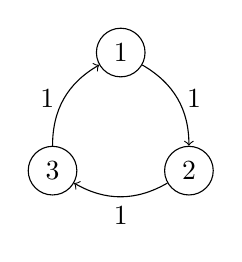
\begin{tikzpicture}[->,node distance=2cm]
                \foreach \i [count=\j from 1] in {90,-30,-150} \node[circle,draw] (\j) at (\i:1) {\j};
                \path (1) edge [bend left] node [right] {1} (2);
                \path (2) edge [bend left] node [below] {1} (3);
                \path (3) edge [bend left] node [left] {1} (1);
            \end{tikzpicture}
        \end{figure}
    \end{minipage} \hfill
    \begin{minipage}{0.45\textwidth}
        $\forall i=1,2,3:$\medskip \\
        $p_{ii}^{(3n)}=1\qquad \forall n+1$\\
        $p_{ii}^{(3n+1)}=0\qquad \forall n\geqslant 1$\\
        $p_{ii}^{(3n+2)}=0\qquad \forall n\geqslant 1$\\
        $d(i)=3 \qquad i\in S$
    \end{minipage}
\end{example}
Periodicity is a \enf{class property}: if $i,j$ communicate then they have the same period. This means that the period of the communication class $S_1$ is enough to study the period of a single $i\in S_1$.
\begin{example}
    The simple random walk is irreducible: $S = \mathbb{Z}$ is a single communicating class. For $i>0$:
    \[
    p_{00}^{(2n)}>0 \qquad p_{00}^{(2n+1)}=0 \qquad n \geqslant 0
    \]
    so the period is 2.
\end{example}

\begin{proposition}
    If $X$ is irreducible and $p_{ii}>0$ for some $i \in S$ then $X$ is aperiodic.
\end{proposition}
\begin{example}
     \begin{minipage}{0.5\textwidth}
        \begin{figure}[H]
            \centering
            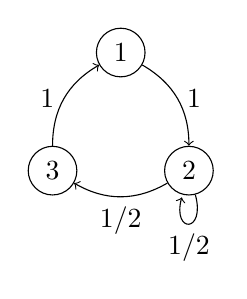
\begin{tikzpicture}[->,node distance=2cm]
                \foreach \i [count=\j from 1] in {90,-30,-150} \node[circle,draw] (\j) at (\i:1) {\j};
                \path (1) edge [bend left] node [right] {1} (2);
                \path (2) edge [bend left] node [below] {1/2} (3);
                \path (3) edge [bend left] node [left] {1} (1);
                \path (2) edge [loop below] node [below] {1/2} (2);
            \end{tikzpicture}
        \end{figure}
    \end{minipage} \hfill
    \begin{minipage}{0.45\textwidth}
        The chain is aperiodic: I can get from 3 back again to 3 in 3 steps of in 4,5,6,$\ldots$ if I cycle in 2.
        \[p_{33}^{(n)}>0\qquad n\geqslant 3.\]
        The greatest common denominator is 1: $d(3)=1$
    \end{minipage}
\end{example}
We can exploit this property: if $P$ is periodic, define
\[
P'=\varepsilon P+(1-\varepsilon)I,\hspace{2cm} \varepsilon\in(0,1)
\]
This is called the "\sott{lazy chain}" because the chain is not going to move from its state in $n$ with probability $\varepsilon$ and $P'$ is aperiodic. We will see that this modification essentially does not alter the distributional properties of the chain. 
\subsubsection{Recurrence}
Recall now the first visit to $i$
\[
T_i=\inf\{n\geqslant 1: X_n=i\}
\]

\begin{definition}
    A state $i$ is said do be \enf{recurrent} if \[\prob(T_i<\infty|X_0=i)=1\],  or equivalently \[\prob(T_i<\infty \quad\text{for some}\quad n|X_0=i)=1\] which means that the return time is finite almost surely. The state $i$ is otherwise said to be \enf{transient}.
\end{definition}
A transient $i$ is such that \[\prob(T_i<\infty|X_0=i)<1.\]It is worth noting that a transient state still has a positive probability of coming back on $\infty$.

\begin{proposition}
    Let $p_{ii}^{(n)}$ be the return probability to $i$ in $n$ steps. Then $i \in S$ is recurrent if and only if \[\sum_{n\geqslant 1} p_{ii}^{(n)}=\infty \] and it is transient otherwise.
\end{proposition}
Let $I_n=\mathbbm{1}(X_n=i)$:
\begin{align*}
    \sum_{n\geqslant 1} p_{ii}^{(n)}&=\sum_{n\geqslant 1} \prob(X_n|X_0=i)\\
    &=\lim_{N \to \infty}\sum_{n=1}^N\ev{I_n|X_0=i}\\
    &=\lim_{N \to \infty}\ev{\underbrace{\sum_{n=1}^NI_n}_{\mathclap{f_N}}|X_0=i}\\
    &=\ev{\sum_{n=1}^{\infty}I_n|X_0=i}\\
    &\text{\footnotesize(by monotone convergence theorem)}
\end{align*}
So $i$ is recurrent if in expectation it is visited $\infty$ many times over the whole time horizon. \\
We can define \[G:=\sum_{n\geqslant 0}p^n\] which is sometimes called \sott{potential matrix}.

\begin{proposition}
    A state $i$ is visited almost surely:
    \begin{itemize}
        \item infinitely often if recurrent;
        \item finitely often if transient
    \end{itemize}
\end{proposition}
Intuition: $T_i^{(1)}$ is the first passage time to $i$. If $i$ is recurrent then by definition
\[
\prob(T_i^{(1)}<\infty|X_0=i)=1.
\]
Since $X_{T_i^{(1)}}=i$, from the strong Markov property we get: \[X'=X_{T_i^{(1)}+n}\sim Markov(\delta_i,P)\]
so $X_{T_i^{(2)}}$ for $X$ is the first passage time for $X'$, which implies 
\[T_i^{(1)}\stackrel{d}{=}T_i^{(2)} \implies \prob(T_i^{(2)}<\infty|X_{T_i^{(1)}}=i)=1.\]
So over an infinite time horizon we have infinitely many visits with probability 1.

Recurrence is a class property, so if a chain is irreducible it is enough to check one state. If we checked that $i$ is recurrent all states that communicate with $i$ will be visited infinitely many times.

\begin{proposition}
    The simple random walk on $\mathbb{Z}$ is recurrent if and only if $p=\frac{1}{2}$, that is if the walk is symmetric. 
\end{proposition}

    \begin{proof2}
        To check that the chain is irreducible, it is enough to check that $i=0$ is irreducible:
        \[p_{00}^{(2n)}>0 \hspace{2cm}  p_{00}^{(2n+1)}=0 \qquad n\geqslant 1\] so it is enough to check the even number of steps:
        \begin{center}
            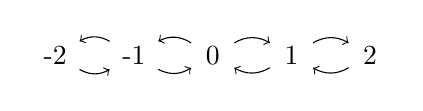
\begin{tikzpicture}[->]
                \node [circle] (zero) {0};
                \node [circle] (one) [right of=zero] {1};
                \node [circle] (two) [right of=one] {2};
                \node [circle] (mone) [left of=zero] {-1};
                \node [circle] (mtwo) [left of=mone] {-2};
                \path (zero) edge [bend left] node [right] {} (one);
                \path (one) edge [bend left] node [right] {} (two);
                \path (zero) edge [bend right] node [right] {} (mone);
                \path (mone) edge [bend right] node [right] {} (mtwo);
                \path (mtwo) edge [bend right] node [right] {} (mone);
                \path (mone) edge [bend right] node [right] {} (zero);
                \path (two) edge [bend left] node [right] {} (one);
                \path (one) edge [bend left] node [right] {} (zero);
            \end{tikzpicture}
        \end{center}
        I sample right and left steps $n$ times each:
        \[p_{00}^{(2n)}=\binom{2n}{n}p^n(1-p)^n\]
        Verify using Stirling's approximation that
        \[n!\approx \text{const}\times n^{n+\frac{1}{2}}e^{-n}\implies p_{00}^{(2n)}\approx \frac{[4p(1-p)]^n}{\sqrt{n}}\]
        so
        \[
            \sum_{n\geqslant 0}p_{00}^{(n)}\approx  \sum_{n\geqslant 0}\frac{[4p(1-p)]^n}{\sqrt{n}}
            \]
            \[
            \rightarrow\begin{cases}
                <\infty &4p(1-p)<1=p(1-p)<\frac{1}{4}\; \text{which means}\;p\neq \frac{1}{2}\\
                =\infty &p=\frac{1}{2}
            \end{cases}
            \]
        which means that the series is infinite when $p=1/2$.
    \end{proof2}
What about a random walk on $\Z^d$? 
\[
d=2,\; i,j\in\Z^2 \qquad p_{ij}=\begin{cases}
    \frac{1}{4} &\text{if}\quad|i_1-j_1|+|i_2-j_2|\\
    0 &\text{else}.
\end{cases}
\]
 \begin{minipage}{0.5\textwidth}
        \begin{tikzpicture}[
            >=stealth', axis/.style={<->},
            point/.style={circle, inner sep=0pt, fill, minimum size=4pt, label=#1},
            scale=.75]
        \draw[axis] (0,-3) -- (0,3) node[above right]{$y$};
        \draw[axis] (-3,0) -- (3,0) node[below right]{$x$};
        \draw[dashed,RedViolet] (0,0) -- (3,3);
        \draw[dashed,RedViolet] (1.5,1.5) -- (3,0);
        \draw[dashed,RedViolet] (0,0) -- (3,-3);
        \draw[dashed,RedViolet] (1.5,-1.5) -- (3,0);
        \coordinate (A) at (1.5,1.5);
        \coordinate (B) at (0,0);
        \draw [|-|]([yshift=0.1cm,xshift=-0.1cm]A) -- ([yshift=0.1cm,xshift=-0.1cm]B)node [black,midway,sloped,above]{$\frac{1}{\sqrt{2}}$};
        \end{tikzpicture}
    \end{minipage} \hfill
    \begin{minipage}{0.45\textwidth}
    The random walk on $\Z^2$ can be seen as 2 independent random walk on the diagonals of the cartesian plane.
    \end{minipage}
\begin{align*}
    &p_{(0,0),(0,0)}^{(2n+1)}=0\\
    &p_{(0,0),(0,0)}^{(2n)}=\Biggl[\underbrace{\binom{2n}{n}\biggl(\frac{1}{2}\biggr)^n\biggl(\frac{1}{2}\biggr)^n}_{\mathclap{\approx \frac{1}{\sqrt{n}}}}\Biggr]^2\\
    &\sum_{n \geqslant 0}p_{(0,0),(0,0)}^{(n)}=\infty\implies\text{the chain is recurrent.}
\end{align*}
Consider now a symmetric random walk on $\Z^3$:
\[
    \sum_{n \geqslant 0}p_{(0,0,0),(0,0,0)}^{(n)}=\Biggl[\underbrace{\binom{2n}{n}\biggl(\frac{1}{2}\biggr)^n\biggl(\frac{1}{2}\biggr)^n}_{\mathclap{\approx \frac{1}{\sqrt{n}}}}\Biggr]^3\approx\frac{1}{n^{\frac{3}{2}}}
\]
This is a convergent series, which means that from 3 dimensions onward the random walk \textit{is transient}.

In the transient case we have:
\[
\sum_{n\geqslant 1}p_{ii}^{(n)}<\infty\implies p_{ii}^{(n)}\xrightarrow[n\rightarrow\infty]{}0
\]
It can be proved that $\forall j \in S$, $p_{ii}^{(n)}\xrightarrow[n\rightarrow\infty]{}0$. In the recurrent case, where we have $\sum p_{ii}^{(n)}=\infty$:
\begin{itemize}
    \item $p_{ii}^{(n)}\rightarrow c>0$, which causes the \textit{divergence} of the series;
    \item  $p_{ii}^{(n)}\rightarrow 0$ but slowly, not faster than $\frac{1}{n}$, causing divergence in this case as well.
\end{itemize}
But is this dichotomy useful? define
\[m_i=\ev{T_i|X_0=i}\] as the \enf{mean return time to} $\enf{i}$. If $i$ is transient, then \[\prob(T_i<\infty|X_0=i)<1\implies\prob(T_i=\infty|X_0=i)>0\implies m_i=\infty\].

\begin{definition}
    A recurrent state $i$ is called:
    \begin{itemize}
        \item \enf{positive} if $m_i<\infty$
        \item \enf{null} if $m_i=\infty$
    \end{itemize}
    and these are \textit{class properties}.
\end{definition}
Later we will show that a \sott{null recurrent} state $i$ is such that $p_{ji}^{(n)}\rightarrow 0$ $\forall j\in S$, so transient and null/positive recurrence can be understood in terms of the \sott{tail of the distribution} of the return times:
\begin{itemize}[-]
    \item positive probability at $\infty$ $\rightarrow$ transience
    \item probability mass is on $\N$ but it is not integrable ("heavy tailed") $\rightarrow$ null recurrence
    \item probability mass is on $\N$ and it is integrable $\rightarrow$ positive recurrence
\end{itemize}
\begin{example}
    The symmetric random walk on $\Z$ and $\Z^2$ are the only recurrent cases:
    \[p_{00}^{(2n)}\propto\frac{1}{\sqrt{n}} \hspace{2.7cm} p_{(0,0),(0,0)}^{2n}\propto\frac{1}{n} \]
    Both tend to 0 as $n$ tends to $\infty$, which means that both the states are null recurrent.
\end{example}
We are now interested in establishing how a chain can be classified as positive recurrent.

\begin{proposition}
    On a finite $S$, an irreducible chain is positive recurrent.
\end{proposition}
    \begin{proof2}
        \[S=\{0,\ldots,N\}\]
        \[\forall n\geqslant1:\qquad\sum_{j=0}^N p_{ij}^{(n)}=1. \]
        This means that we cannot have $p_{ji}^{(n)}\rightarrow 0$ $\forall j\in S$. So there exist a state $i \in S$ that is both positive and irreducible and therefore $X$ must be positive
    \end{proof2} 
\begin{example}
    Consider a Wright-Fisher chain with $S={0,\ldots,N}$. It has:
    \begin{align*}
        X_n=0 &\implies X_{n+1}=0\\
        X_n= &\implies X_{n+1}
    \end{align*}
    so $S$ is finite but $X$ is not irreducible.
    \[
    \begin{tikzpicture}[->,>=stealth',shorten >=2pt, line width=0.5pt, node distance=1.5cm]
        \node[circle, draw](1){$S_1$};
        \node[circle, draw](2)[above right of=1]{$S_2$};
        \node[circle, draw](3)[below right of=1]{$S_3$};
        \path (1) edge (2);
        \path (1) edge (3);
        \node[text width=4cm] [below of=3] {Case without off mutations};
    \end{tikzpicture}\hspace{3cm}
     \begin{tikzpicture}[<->,>=stealth',shorten >=2pt, line width=0.5pt, node distance=1.5cm]
        \node[circle, draw](1){$S_1$};
        \node[circle, draw](2)[above right of=1]{$S_2$};
        \node[circle, draw](3)[below right of=1]{$S_3$};
        \path (1) edge (2);
        \path (1) edge (3);
        \node[text width=4cm] [below of=3] {Case with odd mutations;};
    \end{tikzpicture}
    \]
    More generally, the task can be difficult. Often, so-called \textit{Lypaunov methods} are useful as a sufficient conidition.
\end{example}

\begin{proposition}
    Let $P$ be irreducible and let $h:S\rightarrow\R$ be such that $h(i)\geqslant0 \;\forall i \in S$ and:
    \begin{itemize}
        \item $\sum_{k\in S} p_{ik} \cdot h(k)<\infty\qquad\forall i \in S_0$
        \item $\sum_{k\in S} p_{ik} \cdot h(k)\leqslant h(i)\cdot \varepsilon\qquad\forall i \notin S_0$
    \end{itemize}
    for a finite set $S_0 \subset S$ and some $\varepsilon>0$. Then $P$ is positive recurrent.
\end{proposition}
The role of $h(\cdot)$ is similar to the one of Lyopunov function used for the stability of ODEs. Here
\[\sum_{k} p_{ik} \cdot h(k)-\ev{h(x_{n+1}|X_n=1)}\]
The second condition says that $h(\cdot)$ decreases in expectation outside $S_0$: $S_0$ is \enf{attractive}.
\begin{example}
    $S+\Z_+, \qquad h(i)=i$. The condition requires
    \[\ev{X_{n+1}-X_{n}|X_n=1}<0, \qquad i>i_0\]
    so the chain is atracted to the set $\{i:i\leqslant i_0\}$, giving stochastic stability.
\end{example}
\subsubsection{Stationarity}
Note:
\begin{align*}
    \prob(X_n=j) &= \overbrace{\sum_{i\in S}\prob(X_0=i)\prob(X_n=j|P_0=i) }^{\mathclap{\text{disintegrating the joint}}}\\
    &=\sum_{i\in S}\lambda_i p_{ij}^{(n)}=\left(\lambda P^n\right)_j
\end{align*}
$\left(\lambda P^n\right)_j$ can be seen as the marginal distribution of $X$ at time $n$: in other words
\[X_0\sim \lambda\implies X_n\sim\lambda P^n\]

\begin{definition}
    A non negative (row) vector $\pi=(\pi_i, i\in S)$ is said to be an \enf{invariant measure} for $P$ if $\pi P=\pi$, called \enf{global balance equation}. Namely:
    \[\sum_{i \in S} \pi_i p_{oj}=\pi_j \]
    i.e. marginalizing out the initial state with respect to $\pi$, the marginal measure after one step is preserved:
    \[
    X_0 \sim \pi \implies X_i \sim \pi P = \pi
    \]
\end{definition}
Furthermore,
\[
\pi P^2=\underbrace{\pi P}_{\pi}=\pi P= \pi
\]
Iterativity yields that $\pi P^n=\pi$, therefore
\[
X_0\sim \pi \implies X_n\sim\pi \qquad \forall n \geqslant 0
\]
We have extended the one-step invariance to the $n$-step invariance. If we can normalize $\pi$:
\[
\Tilde{\pi}_i=\frac{\pi_i}{\sum_{j\in S}\pi_j}\Tilde{\pi}\]
and we call $\Tilde{\pi}$ \enf{stationary distribution}.
\begin{example}
        \begin{figure}[H]
            \centering
            \begin{tikzpicture}[->,>=stealth',shorten >=2pt, line width=0.5pt, node distance=2cm]
                \node [circle, draw] (zero) {0};
                \node [circle, draw] (one) [right of=zero] {1};
                \path (zero) edge [bend left] node [above] {$\alpha$} (one);
                \path (zero) edge [loop left] node [left] {$1-\alpha$} (zero);
                \path (one) edge [loop right] node [right] {$1-\beta$} (zero);
                \path (one) edge [bend left] node [below] {$\beta$} (zero);
            \end{tikzpicture}
        \end{figure}
 with $\pi=(\pi_0,\pi_1)$, $\pi_i>0$.
    We need to try and solve the global balance equation:
    \[
    \pi P=\begin{bmatrix}
        \pi_0 & \pi_1
        \end{bmatrix}\begin{bmatrix}
            1-\alpha & \alpha \\
            \beta & 1-\beta
        \end{bmatrix}=\begin{bmatrix}
            \pi_0(1-\alpha)+\pi_1\beta & \pi_0\alpha+\pi_1(1-\beta)
        \end{bmatrix}.
    \]
    Impose $\pi P=\pi=(\pi_0, \pi_1)$:
    \[
    \pi_0(1-\alpha)+\pi_1\beta=\pi_0 \implies \pi_0=\pi_1\frac{\beta}{\alpha}.
    \]
    Substituting,
    \[
    \pi_1\frac{\beta}{\cancel{\alpha}}\cancel{\alpha}+\pi_1\beta=\pi_1 \implies \pi_1=\pi_1 \quad\tikz\fill[scale=0.4](0,.35) -- (.25,0) -- (1,.7) -- (.25,.15) -- cycle;
    \]
    with normalization we get
    \begin{align*}
        \pi_0+\pi_1=1&\longrightarrow{}\pi_1\frac{\beta}{\alpha}+\pi_1=1\\
        &\longrightarrow\pi_1=\frac{\beta}{\alpha+\beta},\quad\pi_0=\frac{\alpha}{\alpha+\beta}.
    \end{align*}
\end{example}
\begin{example}
    If $P$ is stationary with respect to $\pi$ then its "lazy" version \[P'=\varepsilon P+(1-\varepsilon)I,\quad\varepsilon\in[0,1]\]is still stationary.
\end{example}
\begin{example}
    Consider the random walk on $\Z$. The global balance equation is:
    \begin{align*}
        \sum_{i \in S} \pi_i p_{ij}&=\pi_{j-1}p_{j-1,j}+\pi_{j+1}p_{j+1,j}\\
        &=\pi_{j-1}p+\pi_{j+1}(1-p)\stackrel{?}{=}\pi_j
    \end{align*}
    Set $\pi_i=c\geqslant0$:
    \[cp+c(1-p)=c\]
    So:\begin{itemize}
        \item the uniform measure on $\Z$ is invariant;
        \item the invariant measures are not necessarily unique;
        \item $p\neq\frac{1}{2}$ is the transient case, $p=\frac{1}{2}$ is the recurrent case.
    \end{itemize}
    So there exists an invariant measure that doesn't imply recurrence.
    \[
    \sum_{i\in\Z}\pi_i=\begin{cases}
        \infty &c>0\\
        0 &c=0
    \end{cases}
    \]
    We cannot normalize in this case ($\pi$ is only $\sigma$-finite, not finite) so we have invariant measures but we don't have any stationary distribution: the chain is \sott{non stationary}.
\end{example}
\begin{exercise}
    Find the stationary distribution for $RW(p,1-p)$ and $p_{00}=1-p$ under correct restrictions on $p$.
\end{exercise}
\begin{exercise}
    Do the same for $B\&D(p,1-p)$ and $p_{00}=1-p$ under the correct restrictions on $p$.
\end{exercise}
\begin{exercise}
    Show that in $B\&D(p,1-p)$:
    \begin{align*}
        p_i&=\frac{b}{b+i},\quad b>0\\
        \implies\pi_i&=\frac{b+i}{2b}\sim Poiss(i,b)
    \end{align*}
    (called \sott{size-biased Poisson}).
\end{exercise}
We are interested in conditions that provide stationarity:

\begin{proposition}
    If for some $i\in S$ \[
    p_{ij}^{(n)}\xrightarrow[n\rightarrow\infty]{}\pi_j\implies\pi\text{ is invariant.}
    \]
\end{proposition}
    \begin{proof2}
        \[S=\{0,\ldots,N\}\]
        \[\forall n\geqslant1:\qquad\sum_{j=0}^N p_{ij}^{(n)}=1. \]
        This means that we cannot have $p_{ji}^{(n)}\rightarrow 0$ $\forall j\in S$. So there exist a state $i \in S$ that is both positive and irreducible and therefore $X$ must be positive
    \end{proof2} 
\begin{example}
    Consider the random walk on $\Z$:
    \[p_{ij}^{(n)}\rightarrow0\implies\pi=(\pi_i,i\in\Z)\quad\pi_i=0\]
    Which is invariant, as found above, with $c=0$.
\end{example}
\begin{example}
    \[
    P=\begin{bmatrix}
            1-\alpha & \alpha \\
            \beta & 1-\beta
        \end{bmatrix}\qquad\alpha,\beta\neq 1
    \]
    \begin{align*}
        p_{00}^{(n+1)}&\equalexpl{\text{C.K.}}\hspace{1em}\sum_{k\in S}p_{0k}^{(n)}p_{k0}=p_{00}^{(n)}\underbrace{(1-\alpha}_{p_{00}}+\underbrace{pp{01}^{(n)}}_{1-p_{00}^{(n)}}\underbrace{\beta}_{p_{10}}\\
        p_{00}^{(n+1)}&=\ldots=\beta+p_{00}^{(n)}(1-\alpha-\beta)
    \end{align*}
    The recurrence equation brings to solution:
    \[p_{00}^{(n)}=\frac{\beta}{\alpha+\beta}+(1-\alpha-\beta)^n\frac{\alpha}{\alpha+\beta}\rightarrow\frac{\beta}{\alpha+\beta}\]
    as found earlier.
\end{example}
In general we do not want to assume that $P^n$ converges.
\begin{theorem}
     An irreducible Markov Chain has invariant distribution $\pi$ if and only if it is positive recurrent, in which case $\pi$ is unique and 
        \begin{equation*}
            \pi_i = \frac{1}{m_i}
        \end{equation*}
        where 
        \begin{equation*}
            m_i = \ev{T_i | X_0 = i}
        \end{equation*}
        is the \textbf{expected return time}. 
\end{theorem}
\begin{example}
    Considering $P=I$, we found out that the invariant distribution is not unique. This is a contradiction, due to the fact that irreducibility is violated.
\end{example}
\begin{example}
    Consider a random walk on $\mathbb{Z}$ for $p \in (0,1)$ which is transient and null recurrent: This implies that $m_i = \infty$. Indeed $\pi_i = \frac{1}{m_i} = 0$ is invariant for the random walk. 
\end{example}
\begin{example}
    Consider a 2-state chain with
    \begin{equation*}
        (\pi_0, \pi_1) = (\frac{\beta}{\alpha + \beta}, \frac{\alpha}{\alpha + \beta}).
    \end{equation*}
    If we interpret the statement literally, then\[(m_0,m_1)= (\frac{\alpha +\beta}{\beta}, \frac{\alpha + \beta}{\alpha})\]
    Let's choose, for example,  $\alpha = 0.5$ and $\beta = 1$:\[   
    \begin{tikzpicture}[->,>=stealth',shorten >=2pt, line width=0.5pt, node distance=2cm]
        \node [circle, draw] (zero) {0};
        \node [circle, draw] (one) [right of=zero] {1};
        \path (zero) edge [bend left] node [above] {$\frac{1}{2}$} (one);
        \path (zero) edge [loop left] node [left] {$\frac{1}{2}$} (zero);
        \path (one) edge [bend left] node [below] {$1$} (zero);
    \end{tikzpicture}\]
    with $m_0=\frac{3}{2}$ and $m_1=3$
    We can double check:
    \begin{itemize}
        \item Return to 0: $\begin{cases}
            1 &\text{ with probability } \frac{1}{2}\\
            2 &\text{ with probability } \frac{1}{2}\\
        \end{cases}$ $\implies 1 \cdot \frac{1}{2} + 2 \cdot \frac{1}{2} = \frac{3}{2} = m_0$
        \item Return to 1: $\begin{cases}
            2 &\text{ with probability } \frac{1}{2}\\
            3 &\text{ with probability } \frac{1}{2^2}\\
            \vdots \\
            (1+k) &\text{ with probability } \frac{1}{2^k}\\
            \vdots\\
        \end{cases}$
        so\[m_1 = \sum_{k \geq 1} (1+k) \frac{1}{2^k} = \ldots = \sum_{k \geq 1} \frac{1}{2^k} + \sum_{k \geq 1} \frac{k}{2^k} = 1+2 = 3.\]
    \end{itemize}
\end{example}
\begin{definition}
    An irreducible Markov chain is said to be \enf{reversible  with respect to $\pi$} if 
\[
            \pi_i p_{ij} = \pi_j p_{ji} \hspace{1 cm} \forall i,j \in S  \hspace{1 cm} \]
        which is called \enf{detailed balance equation}.
\end{definition}\begin{proposition}
    If $P$ and $\pi$ are in detailed balance (that is, they satisfy the detailed balance equation, then $\pi$ is invariant for $P$.
\end{proposition}
    
    \begin{proof2}
        Integrate both sides of the equation with respect to $i$:
        \begin{align*}
            \sum_i\pi_ip_{ij}&= \sum_i\pi_jp_{ij}\\
            &=\pi_j\underbrace{\sum_ip_{ij}}_{=1}=\pi_j.
        \end{align*}
    \end{proof2}
Detailed balance is a sort of \sott{local criterion} on the chain propensity to go from $i\rightarrow j$ and $j \rightarrow i$, while the global balance is a \sott{global criterion} on the chain propensity to go from $i\rightarrow j$ and $j \rightarrow i$.
\begin{example}
     \begin{minipage}{0.5\textwidth}
     \center
        \begin{tikzpicture}[->,>=stealth',node distance=2cm]
                \foreach \i [count=\j from 0] in {150,30,-90} 
                \node[circle,draw] (\j) at (\i:1.3) {\j};
                \path (0) edge [bend left] node [above] {\footnotesize 2/3} (1);
                \path (1) edge [bend left] node [below right] {\footnotesize 2/3} (2);
                \path (2) edge [bend left] node [below left] {\footnotesize 2/3} (0);
                \path (1) edge [bend left] node [above] {\footnotesize 1/3} (0);
                \path (2) edge [bend left] node [right] {\footnotesize 1/3} (1);
                \path (0) edge [bend left] node [left] {\footnotesize 1/3} (2);
        \end{tikzpicture}
    \end{minipage} \hfill
    \begin{minipage}{0.45\textwidth}
    Check first that the uniform distribution is invariant: \[\pi = (\frac{1}{3}, \frac{1}{3}, \frac{1}{3}).\] 
    Nevertheless, 
    \[
        \pi_0 p_{01} = \frac{1}{3} \frac{2}{3} \neq \frac{1}{3}\frac{1}{3} = \pi_1 p_{10}
    \]
    \end{minipage}
\end{example}
\begin{example}
    Consider a Birth and Death process of parameters $(p,1-p)$ with 
    \begin{equation*}
        p_{00} = 1-p
    \end{equation*}
    The detailed balance equation is
    \begin{equation*}
        \pi_i p_{ij} = \pi_j p_{ji}   \hspace{1 cm} \forall i,j
    \end{equation*}
    Take $j=i+1$: we get
    \begin{align*}
        \pi_i p_{i,i+1} &= \pi_{i+1} p_{i+1,i}  \hspace{1 cm} q:=1-p \\
        \pi_i p &= \pi_{i+1} q\\
        i = 0 &\implies \pi_1 = \pi_0 \frac{p}{q}\\
        i = 1 &\implies \pi_2 = \pi_1 \frac{p}{q} = \pi_0 \Big(\frac{p}{q}\Big)^2 \\
        &\implies \pi_k = \pi_0 \Big(\frac{p}{q}\Big)^k
    \end{align*}
    So, $\pi_k$ is proportional to $\rho^k$, where $\rho = \frac{p}{q}$. \\
    We now integrate $\pi_k$:
    \begin{equation*}
        \sum_{k \geq 0} \pi_k < \infty \iff p < \frac{1}{2} \hspace{0.5 cm} (\rho < 1) + \ldots
    \end{equation*}
    which implies that 
    \begin{equation*}
        \Tilde{\pi} = \frac{\pi_k}{\sum_j \pi_j} \sim \text{Geom}(\rho).
    \end{equation*}
    So, using detailed balance equations, we get a result faster than what we would obtain through global balance equations.
\end{example}
Let 
\begin{equation*}
    <x,y>:= \sum_{i \in S} x_i y_i \pi_i.
\end{equation*}
\begin{definition}
    We define 
        \begin{equation*}
            \ell_2(\pi) := \{x \in \mathbb{R}^S: <x,x> < \infty\}.
        \end{equation*}
        A matrix $P$ is \enf{self-adjoint with respect to} $\pi$ if 
        \begin{equation*}
            <Px,y> = <x, Py>, \hspace{1 cm} x,y \in \ell_2(\pi).
        \end{equation*}
\end{definition}\begin{proposition}
     Markov chain with transition matrix $P$ is reversible with respect to $\pi$ if and only if $P$ is self-adjoint with respect to $\pi$.
\end{proposition}
It can be proved that if $P$ is reversible with respect to $\pi$, then the \enf{time reversal}
        \begin{equation*}
            Y_n := X_{N-n}, \hspace{1 cm} 0 \leqslant n \leqslant N
        \end{equation*}
        has the same distribution as $X$ if both are started in equilibrium.
\subsubsection{Convergence}
We can interpret time reversal as the possibility of reversing the sense of time. If the chain $X$ starts from an arbitrary initial distribution, not necessarily at equilibrium, is it going to converge to the stationary distribution?
\begin{equation*}
    \lambda P^n \xrightarrow[\text{?}]{n \rightarrow \infty} \pi
\end{equation*}
The notion of convergence convergence has to be made more precise.
\begin{example}
    Consider the matrix $P$:\\
    \begin{minipage}{0.5\textwidth}
     \center
        \[P=\begin{bmatrix}
        0 & 1 \\
        1 & 0 \\
    \end{bmatrix}\]
    \end{minipage} \hfill
    \begin{minipage}{0.45\textwidth}
    \begin{figure}[H]
            \centering
            \begin{tikzpicture}[->,>=stealth',shorten >=2pt, line width=0.5pt, node distance=2cm]
                \node [circle, draw] (zero) {0};
                \node [circle, draw] (one) [right of=zero] {1};
                \path (zero) edge [bend left] node [above] {} (one);
                \path (one) edge [bend left] node [below] {} (zero);
            \end{tikzpicture}
        \end{figure}
    \end{minipage}
    The chain is 
    \begin{itemize}
        \item [-] irreducible 
        \item [-] positive-recurrent (the mean return time, which is the only return time, equals $2$)
        \item [-] The stationary distribution
        \begin{equation*}
            \pi = (\frac{1}{2}, \frac{1}{2}) 
        \end{equation*}
        is invariant \checkmark
        \end{itemize}
     But, 
    \begin{itemize}
        \item [-] $P^{2n+1} = P, \;P^{2n} = I$, so $p_{ij}^{(n)} \not\rightarrow \pi_j$. Previously, we assumed convergence and  said that a limiting distribution is invariant
        \item [-] $\lambda P^{2n} = \lambda \hspace{1 cm} \lambda P^{2n+1}=1-\lambda$
    \end{itemize}
    Why? The periodicity is \sott{preventing the chain to converge}. Periodicity prevents convergence by making the dependence on the initial state too strong: if the chain starts from 0 the all even steps will bring to 0 and all odd steps will bring to 1.
\end{example}
\begin{definition}
    An irreducible, aperiodic, positive recurrent chain is called \enf{ergodic}.
\end{definition}
Under these assumptions, we want to show that an ergodic chain converges to equilibrium from any initial distribution. To do so, we are going to use \sott{\textit{coupling}}. Consider
\begin{itemize}
    \item $\pi$ invariant for $P$
    \item $X \sim$ Markov $(\lambda, P)$. $\lambda$ is arbitrary and the so distributed $X$ is the chain of interest.
    \item $Y \sim$ Markov $(\pi, P)$ is an auxiliary chain
    \[\implies Y_n \sim \pi, \forall n \geq 0\]
    \item Assume $X$ and $Y$ meet in finite time.
\end{itemize}
\begin{figure}[H]
    \centering
    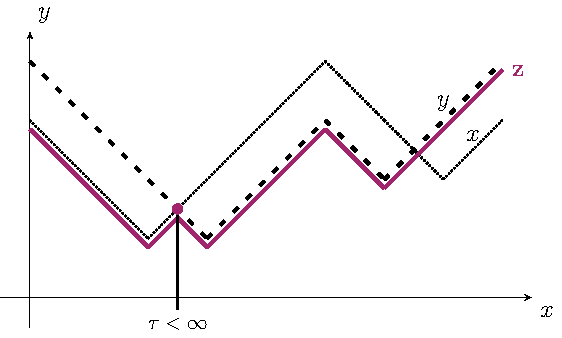
\includegraphics{standalones/pdfs/coupling}
\end{figure}
We obtain a new chain $Z_n$ so defined:
\[
Z_n = 
\begin{cases}
    X_n & n<\tau \\
    Y_n & n \geq \tau \\
\end{cases}
\]
Now, \underline{if} we show that $Z \sim$ Markov $(\lambda, P)$ (reaching quote $2$ assumptions, together with meeting in finite time), then 
\[
    X \stackrel{d}= Z \qquad\text{and}\qquad
    Z_n \sim \pi \hspace{0.5 cm} \forall n \geq \tau\]
which would imply that 
\begin{equation*}
    X_0 \sim \lambda, X_n \xrightarrow{n \rightarrow \infty} \pi 
\end{equation*}
\begin{definition}
    Two Markov chains $Z$ and $Y$ on $S$ are said to \enf{couple} if there exists an almost surely finite stopping time $\tau$, called \enf{coupling time}, such that 
        \begin{equation*}
            Z_n = Y_n \hspace{1 cm} \forall n \geq \tau
        \end{equation*}
\end{definition}
This relates to the \enf{total variation distance} between the marginals:
\begin{equation*}
    V \sim \lambda,\; W \sim \mu \text{ on } S
\end{equation*}
The total variation distance is 
\begin{align*}
    d_{TV}(\lambda,\mu) &= \sup_{A \subset S} |\mathbb{P}(V \in A) - \mathbb{P}(W \in A)| \\
    &= \frac{1}{2} \sum_{i \in S} |\lambda_i - \mu_i|
\end{align*}
\begin{proposition}
    \label{totvardist}
        Let $Z \sim$ Markov$(\lambda, P)$ and 
        let $Y \sim$ Markov$(\mu, P)$; \\
        assume that a coupling time exists. Then,
        \begin{equation*}
            d_{TV}(\lambda P^n, \mu P^n) \xrightarrow{n \rightarrow \infty} 0
        \end{equation*}
\end{proposition}

        \begin{proof2}
            Consider $A \subset S$ and 
        \begin{align*}
            \mathbb{P}(Z_n \in A) - \mathbb{P}(Y_n \in A) &= \mathbb{P}(Z_n \in A, n < \tau) + \mathbb{P}(Z_n \in A, n \geq \tau) +\\
            &- \mathbb{P}(Y_n \in A, n < \tau) - \mathbb{P}(Y_n \in A, n \geq \tau) \\
            &\stackrel{Z_n = Y_n, \forall n \geq \tau}= \mathbb{P}(Z_n \in A, n < \tau)- \underbrace{\mathbb{P}(Y_n \in A, n < \tau)}_{\geq 0} \\
            &\leq \mathbb{P}(\underbrace{Z_n \in A, n < \tau}_{\subset \{n < \tau\}})\\
            &\leq \mathbb{P}(n < \tau)
        \end{align*}
        Hence, by the arbitrarity of $A$,
        \begin{equation*}
            \sup_{A \subset S} |\mathbb{P}(Z_n \in A) - \mathbb{P}(Y_n \in A)| \leq \mathbb{P}(\tau > n)
        \end{equation*}
        but $\tau < \infty$ almost surely, so
        \begin{equation*}
            \mathbb{P}(\tau > n) \xrightarrow{n \rightarrow \infty} 0
        \end{equation*}
        \end{proof2}
So, we are sure that in a finite time they meet and hence $Z$ is going to have the stationary distribution $\pi$. Also, 
\begin{equation*}
    \exists \tau < \infty \implies d_{TV} \rightarrow 0
\end{equation*}
It is enough to show that such $\tau$ exists for ergodic chains. 
\begin{theorem}
     Let 
        \begin{itemize}
            \item $P$ be ergodic 
            \item $X \sim$ Markov$(\lambda, P)$ and $Y \sim $ Markov$(\mu, P)$ be independent 
        \end{itemize}
        Then, the stopping time 
        \begin{equation*}
            \tau = \inf\{n \geq 0: X_n = Y_n\}
        \end{equation*}
        is almost surely finite, and the chain
        \[
        Z_n =   
        \begin{cases}
            X_n & n<\tau \\
            Y_n & n \geq \tau \\
        \end{cases}
        \]
        is Markov$(\lambda, P)$.
\end{theorem}
So, this yields a coupling time between $Z \sim$ Markov$(\lambda, P)$ and $Y \sim$ Markov $(\mu, P)$, which implies that 
\begin{equation*}
    Z_n = Y_n \sim \mu P^n, \forall n \geq \tau
\end{equation*}
So, by the Proposition \ref{totvardist}, 
\begin{equation*}
    d_{TV}(\lambda P^n, \mu P^n) \xrightarrow{n \rightarrow \infty} 0
\end{equation*}
If we now let $\mu = \pi$, then $\mu P^n = \pi$ and hence 
\begin{equation*}
    d_{TV}(\lambda P^n, \pi) \rightarrow 0
\end{equation*}
\begin{remark}
        Imposing $\mu = \pi$ is not cheating since $\mu$ is auxiliary and we can equal it to what we need. The result is that all the marginals converge to the stationary. 
\end{remark}
Since $X \stackrel{d} = Z$, then
\begin{equation*}
    \mathbb{P}(X_n = j) \xrightarrow{n \rightarrow \infty} \pi_j, \hspace{1 cm} \text{ for every initial distribution } \lambda
\end{equation*}
If $\lambda = \delta_i$:
\begin{align*}
    d_{TV}(\lambda P^n, \pi) &= \frac{1}{2} \sum_{j \in S} |(\lambda P^n)_j - \pi_j| \\
    &= \frac{1}{2} \sum_{j \in S} |\sum_h \lambda_h p_{hj}^{(n)} - \pi_j| \\
    &= \frac{1}{2} \sum_{j \in S} |1 \cdot p_{ij}^{(n)}-\pi_j| \xrightarrow{n \rightarrow \infty} 0
\end{align*}
\begin{remark}
        In the first line, we take the supremum over a discrete space, so in the worst case we integrate the differences. 
\end{remark}
Hence, all the transition probabilities 
\begin{equation*}
    p_{ij}^{(n)} \xrightarrow{n \rightarrow \infty} \pi_j, \forall i \in S
\end{equation*}
converge to $\pi_j$ for every starting point (state) $i$.\\
In summary:
\begin{theorem}
    \label{th erg}
        Let $P$ be ergodic with invariant distribution $\pi$, and let $X \sim$ Markov$(\lambda, P)$. Then,
        \begin{equation*}
            d_{TV}(\lambda P^n, \pi) \xrightarrow{n \rightarrow \infty} 0
        \end{equation*}
        and
        \begin{equation*}
            p_{ij}^{(n)} \xrightarrow{n \rightarrow \infty} \pi_j, \hspace{1 cm} \forall i,j \in S. 
        \end{equation*}
\end{theorem}
\begin{remark}
        Ergodicity ensures that the two chains meet on the diagonal. $\lambda$ is orthogonal to $\mu$ and there exists $B \in S$ such that 
    \begin{align*}
        &\sum_{i \in B} \lambda_i = 1 \\
        &\sum_{i \in B^C} \mu_i = 1 \\
    \end{align*}
\end{remark}
\begin{example}
     Consider the matrix $P$:\\
    \begin{minipage}{0.5\textwidth}
     \center
        \[P=\begin{bmatrix}
        0 & 1 \\
        1 & 0 \\
    \end{bmatrix}\]
    \end{minipage} \hfill
    \begin{minipage}{0.45\textwidth}
    \begin{figure}[H]
            \centering
            \begin{tikzpicture}[->,>=stealth',shorten >=2pt, line width=0.5pt, node distance=2cm]
                \node [circle, draw] (zero) {0};
                \node [circle, draw] (one) [right of=zero] {1};
                \path (zero) edge [bend left] node [above] {} (one);
                \path (one) edge [bend left] node [below] {} (zero);
            \end{tikzpicture}
        \end{figure}
    \end{minipage}
    We know that \[
        \pi = (\frac{1}{2}, \frac{1}{2}) \qquad\text{and}\qquad P^{(2n)} = I, P^{(2n+1)} = P \]
    Consider also $X, Y$ as characterized in Theorem \ref{th erg}, with $\lambda = \delta_0, \mu = \pi$. This means that $X$ starts at $0$ with probability $1$:
    \begin{align*}
        X_0 &= 0 \text{ a.s.} \\
        Y_0 &=
        \begin{cases}
            0 &\text{ with probability } \frac{1}{2} \\
            1 &\text{ with probability } \frac{1}{2} \\
        \end{cases}
    \end{align*}
    So, either they meet at $n = 0$ or they never meet. 
\end{example}
It's useful to remind that are talking about almost sure meeting, not with probability $1$. Which factor breaks the conclusion of meeting almost surely? The chain is:
\begin{itemize}
    \item positive recurrent;
    \item irreducible;
    \item \sott{not} aperiodic.
\end{itemize}
\begin{theorem}
    \enf{Ergodic theorem}. Let $X\sim Markov(\lambda,P)$ be irreducible and let $m_i=\mathbb{E}\Bigl[T_i|X_0=i\Bigr]$. Then, almost surely,
        \[\frac{1}{N}\sum_{n=1}^N\mathbbm{1}(X_n=j)\xrightarrow[N\rightarrow\infty]{}\Pi_j=\frac{1}{m_j}.\]
        Moreover, if $P$ is positive recurrent with unique stationary distribution $\pi$ and $f:S\rightarrow\mathbb{R}$ with respect to $\pi$, then
        \[\frac{1}{N}\sum_{n=1}^Nf(X_n)\xrightarrow[N\rightarrow\infty]{}\sum_{j\in S}f(j)\Pi_j.\]
\end{theorem}
The quantity $\frac{1}{N}\sum_{n=1}^Nf(X_n)$ is the \textbf{ergodic average} and it is taken along the sample path of the chain. The right-hand side shows an object whose form recalls an expectation. \\
So, this is a way of relaxing the assumption of an i.i.d. sample. We are substituting it with the correlation associated to the Markovian structure, so that the convergence holds. 
\[\sum_{j\in S}f(j)\Pi_j=\ev{f(X_n)} \qquad \text{at equilibrium.}\]
So we have an equivalent form of the Strong Law of Large numbers for Markov Chains.
\begin{remark}
    In the one-dimensional case, we have convergence of order $\frac{1}{\sqrt{10}}$ to $0$, which is not enough to make $m_j < \infty$. Hence $m_j = \infty \implies \frac{1}{m_i} \rightarrow 0$, which is consistent with what we know.
\end{remark}
The first claim holds for all irreducible chains, for example the Random Walk whereby:
\[p_{00}^{(n)}\rightarrow0 \qquad\text{as }\frac{1}{\sqrt{n}}\text{ and }m_i=\infty\]
implies
\[\frac{1}{N}\sum_n\mathbbm{1}(X_n=j)\rightarrow0.\]
What about the speed of convergence?
\begin{example}
    Consider \[   P=\begin{bmatrix}
            1-\alpha & \alpha \\
            \beta & 1-\beta
        \end{bmatrix}\]
With
\[
p_{00}^{(n)}=\frac{\beta}{\alpha+\beta}+(1-\alpha-\beta)^n\frac{\alpha}{\alpha+\beta}.
\]
Set $\gamma_1=1$ and $\gamma_2=1-\alpha-\beta$.
We can prove that
\begin{align*}
    P^n &=\frac{1}{\alpha+\beta}\begin{bmatrix}
            \beta & \alpha \\
            \beta & \alpha
        \end{bmatrix}=\frac{1-\alpha-\beta}{\alpha+\beta}\begin{bmatrix}
           & \\
         & \\
        \end{bmatrix}\\
        \pi &=\mathbf{1}^T=\begin{bmatrix}
            \pi_0 & \pi_1 \\
            \pi_0 & \pi_1
        \end{bmatrix}\\
        P^n-\pi=\gamma_2^n B
\end{align*} %boooh non ho mica tanto capito
\end{example}
\begin{theorem}
    Let $P$ be a $k\times k$ irreducible and aperiodic transition matrix. Denote the distinct eigenvalues as
        \[1=\gamma_1>|\gamma_2|>|\gamma_3|>\ldots>|\gamma_k|.\]Then
        \[P^n=\pi+
    \mathcal{O}(n^{m-1}|\gamma_2|^n)\] where $m$ is the algebraic multiplicity of $\gamma_2$.
\end{theorem}
\begin{definition}
    A statement like\[
        d_{TV}(\lambda P^n,\pi)\leqslant C(\lambda)\rho^n
        \] is called \textbf{geometric ergodicity}, with $C(\lambda)\in\R$ depending on $\lambda$.
\end{definition}
\subsubsection{Quasi-stationary distributions}
Let's now take into account \textbf{quasi-stationary distributions}.\\
Let $a\in S$ be an absorbing state with $\prob(T_a<\infty)=1$ visited almost surely in finite time. if $X$ is irreducible then there is no stationarity.\\
\textbf{Example}: the Galton-Watson branching process with mean offspring $m=\ev{g}<1$.
It could be of interest to study the behaviour before absorption.\\
Let $\lambda$ be supported by $S_a=S/\{a\}$ and denote\[\prob_\lambda(\cdot):=\prob(\cdot|X_0\sim\lambda).\] Then, given $A\subset S_a$, we are interested in 
\[\prob_\lambda(X_n\in A|T_a>n)=\frac{\prob_\lambda(X_n\in A,T_a>n)}{\prob_\lambda(T_a>n)}=\frac{\lambda P^n|_a}{\lambda P^n|_{S_a}}.\]
\begin{definition}
     We say that $\pi$ is a \textbf{quasi-stationary distribution} if
        \[
        P_\pi (X_n=i|T_a>n)=\Pi_i\qquad \forall n \geqslant 0.
        \]
        This process preserves the marginal, conditional on not getting observed.
\end{definition}
\begin{example}
    With $S=\{0,\dots,N\}$, let $Y$ be a symmetric random walk on $S_0=\{1,\ldots,N\}$:
\begin{figure}[H]
    \centering
    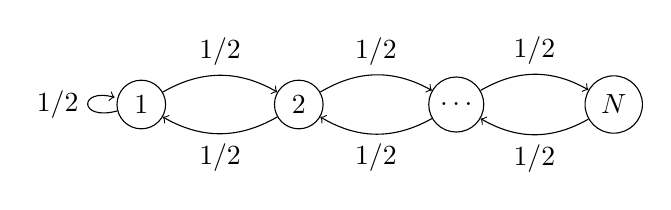
\begin{tikzpicture}[->,node distance=2cm]
                \node [circle,draw] (one) [] {1};
                \node [circle,draw] (two) [right of=one] {2};
                \node [circle,draw] (dots) [right of=two]{$\ldots$};
                \node [circle,draw] (enne) [right of=dots] {$N$};
                \path (one) edge [bend left] node [above] {1/2} (two);
                \path (two) edge [bend left] node [above] {1/2} (dots);
                \path (dots) edge [bend left] node [above] {1/2} (enne);
                \path (enne) edge [bend left] node [below] {1/2} (dots);
                \path (dots) edge [bend left] node [below] {1/2} (two);
                \path (two) edge [bend left] node [below] {1/2} (one);
                \path (one) edge [loop left] node [left] {1/2} (one);
            \end{tikzpicture}
    \label{symmrw}
\end{figure} whose invariant $\pi$ is the uniform on on $S_0$. Let $\tau$ be a finite random time on $\N$, independent of $Y$, such that:
\[
X_n=\begin{cases}
    Y_n &n<\tau\\
    0 &n>\tau
\end{cases}.
\]
So, in $\tau$, $X$ jumps to 0 and there remains. The transition probabilities are:
\[
i \in S_0:\;p_{ij}^{(n)}=\underbrace{\begin{cases}
    \prob(\tau=n)&j=0\\
    \frac{1}{2}(1-\prob(\tau-n)) &j=i\pm 1
\end{cases}}_{\text{there are called \textit{modulo boundaries}}}
\]
Since $\tau$ is independent, we have 
\begin{align*}
    \prob_{\pi}(X_n=i|\tau>n)&=\prob_{\pi}(X_n=i|X_n\neq0)\\
    &=\prob_{\pi}(Y_n=i)=\Pi_i
\end{align*}
\end{example}
\subsection{Hidden Markov Chains}
Hidden Markov Chains are a widely applied statistical framework, useful whenever it is necessary to estimate the current status of a system based on noisy or incomplete observations.

\textbf{Examples}:\begin{itemize}
    \item $X_n$: position of a moving object;\\
    $Y_n$: noisy observations of the position (by means, for instance, of a radar or a sonar);
    \item $X_n$: state of a productive system (that can be good or bad);\\
    $Y_n$: conditions of the output (that can be perfect or faulty);
    \item $X_n$: latent level of volatility in a financial market (high or low);\\
    $Y_n$: amount of financial products exchanged;
    \item $X_n$: number of alleles of type 0 in a population;\\
    $Y_n$: number of alleles of type 0 in a sample;
\end{itemize}
Let $X\sim Markov(\lambda, P)$ be unobserved (or hidden). This chain is sometimes called \textit{signal}. Every time $X$ enters a sate, an observation $Y$ (that we assume discrete on $\{a_1, a_2,\ldots\}$) is emitted with probability that depends on the current state of $X$ only. The model is:
\begin{align*}
    &\diamond \prob(X_n=j|X_{n-1}+i)=p_{ij}\\
    &\diamond \prob(\underbrace{Y_n=y_n}_{\mathclap{\text{generic realization of }Y}}|X_n=j)=p_j(y_n)
\end{align*}
$p_j(y_n)$ is the \textbf{emission distribution}, that is the likelihood of observing $Y_n$ if $X$ is in $j$. If $S+\{0,1\}$:
\begin{figure}[H]
    \centering
    \begin{tikzpicture}[->,>=stealth', line width=0.5pt, node distance=2cm]
        \node [circle,draw] (0) [] {0};
        \node [circle,draw] (a1) [below left=1.5cm and 0.2 cm of 0] {$a_1$};
        \node [circle,draw] (a2) [below right=1.5cm and 0.2 cm of 0]{$a_2$};
        \node [circle,draw] (1) [above right=1.5cm and 0.2 cm of a2] {1};
        \node [circle,draw] (a3) [below right=1.5cm and 0.2 cm  of 1] {$a_3$};
        \path (0) edge [black] node [above,midway,sloped] {\footnotesize$p_0(a_1)$} (a1);
        \path (0) edge [black] node [above,near end,sloped, rotate=180] {\footnotesize$\ldots$} (a2);
        \path (0) edge [black] node [above,near end,sloped, rotate=180] {\footnotesize$\ldots$} (a3);
        \path (1) edge [RedViolet] node [RedViolet,above,midway,sloped] {\footnotesize$p_1(a_3)$} (a3);
        \path (1) edge [RedViolet] node [RedViolet,above,near start,sloped, rotate=180] {\footnotesize$\ldots$} (a2);
        \path (1) edge [RedViolet] node [RedViolet,above,near start,sloped, rotate=180] {\footnotesize$\ldots$} (a1);
        \path (0) edge [bend left] node {} (1);
        \path (1) edge [bend left] node {} (0);
        \path (0) edge [loop left] node {} (0);
        \path (1) edge [loop right] node {} (1);
    \end{tikzpicture}
    \label{hidden}
\end{figure}
An alternative depiction is:
\begin{figure}[H]
    \centering
       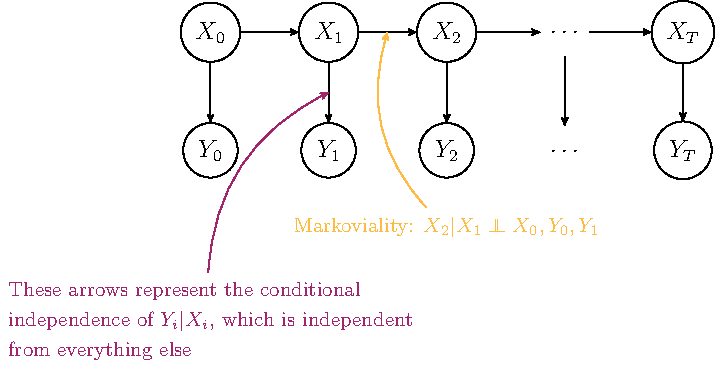
\includegraphics{standalones/pdfs/hid}
    \label{hiddalt}
\end{figure}
The goal is to establish
\begin{align*}
    &\prob(X_{0:T}|Y_{0:T})\\
    \text{with}\quad &X_{0:T}=(X_0,\ldots,X_T)\\
    &Y_{0:T}=(Y_0,\ldots,Y_T)
\end{align*}
as the probability of a certain sequence of states of the system, given a sequence of observations. We can use the chain rule to write:
\[
\prob(X_T|Y_{0:T})\prob(X_{T-1}|X_T,Y_{0:T})\cdot\ldots\cdot\prob(X_0|X_{1:T},Y_{0:T})
\]
as the backwards decomposition. The generic factor is:
\begin{equation*}
    \prob(X_n|X_{n+1:T},Y_{0:T})=\prob(\underbrace{X_n|Y_{0:T}}_{\mathclap{Z}},\underbrace{X_{n+1}}_{W})
\end{equation*}
by virtue of the fact that $X_n|X_{n+1:T}\perp X_{n+2:T},Y_{n+1:T}$. By Bayes' theorem:
\begin{align*}
    \prob(Z|W)&\propto\prob(Z)\prob(W|Z)\\
    &\propto\prob(X_n|Y_{0:n})\prob(X_{n+1}|X_n,Y_{0:n})\\
    &=\prob(X_n|Y_{0:n})\prob(X_{n+1}|X_n)
\end{align*}
Since $X_{n+1}|X_n$ is independent from everything. $\prob(X_n|Y_{0:n})$ is the \textbf{filtering distribution}, the conditional law of $X$ given the information of past and present data, while $\prob(X_{n+1}|X_n)$ is the transition probability of $X$. \\Define
\[F_n(j)=\prob(X_n=j,Y_{0:n})\] so that
\[
\prob(X_n|Y_{0:n})=\frac{F_n(j)}{\sum_i F_n(i)}.
\]
Then
\begin{align*}
    F_n(j)&=\prob(Y_{0:n-1},X_n=j,Y_n=y_n)\\
    &=\sum_i\prob(\underbrace{Y_{0:n-1},X_{n-1}=i}_{F_{n-1}(i)},X_n=j,Y_n=y_n)\\
    &=\sum_i F_{n-1}(i)\underbrace{\prob(X_n=j,Y_n=y_n|X_{n-1}=i,Y_{0:n-1})}_{\prob(X_n|X_{n-1})\prob(Y_n|X_n)}\\
    &=\sum_i F_{n-1}(i)p_{ij}p_j(y_n)\\
    &\implies F_n(j)+\Bigl(\sum_iF_{n-1}(i)p_{ij}\Bigr)p_j(y_n)
\end{align*}
So that these can be computed recursively.
\begin{align*}
    F_0(j)&=\prob(X_0=j,Y_0)=\lambda_jp_j(y_0)\\
    F_1(j)&=\sum_i F_0(i)p_{ij}p_j(y_1)\\
    &=p_j(y_1)\sum_i\lambda_i p_i(y_0)p_{ij}
\end{align*}
If $S$ is finite, we can compute these quantities. Normalizing, we get the filtering distribution
\[
\prob(X_n=j|Y_{0:n})=\frac{F_n(j)}{\sum_i F_n(i)}.
\]
Moreover, if we consider the \textbf{marginal smoothing distribution}
\begin{align*}
    \prob(X_n|y_{0:n})&=\prob(\underbrace{X_n|Y_{0:n}}_{Z},\underbrace{Y_{n+1:T}}_{W})\\
    &\propto\prob(Z)\prob(W|Z)\qquad\text{since }Y_{n+1:T}|X_n \independent Y_{0:n}\\
    &=\underbrace{\prob(X_n|Y_{0:n})}_{\mathclap{\text{filtering distribution}}}\overbrace{\prob(Y_{n+1:T}|X_n)}^{\mathclap{B_n(\cdot)}}.
\end{align*}
$B_n(\cdot)$ is the \textbf{cost-to-go} function: it measures the likelihood of the future observations given a state of $X$:
\[B_n(j)+\prob(Y_{n+1:T}|X_n=j)\]
with
\[
\prob(X_n|Y_{0:T})\propto F_n(j)B_n(j).
\]
Also, $B_n$ can be computed recursively as
\[B_n(j)=\sum_i p_{ij}p_{j}(y_{n+1})B_{n+1}(j)\]
starting from $T$ and proceeding backwards. Finally, with these we have
\[
\prob(Y_{0:T})=\sum_jF_n(j)B_n(j)
\]
which represents the likelihood of the observations, which in principle can be maximized.
\subsection{General state space}
Assume for simplicity that $S\subset\R$ or $\R^k$ (uncountable). Define a time-homogeneous transition probability from 
\[\prob(x,A):=\prob(X_{n+1}\in A|X_n=x),\qquad A\in\mathscr{B}(S).\]
If this has a density with respect to some dominant measure $\nu$, we call
\[p=\frac{dP}{d\nu}\]
the \textbf{transition density}.\\
For example, if $\nu$ is the Lebesgue measure,
\[\prob(x,A)=\int_A \prob(x.y)dy\].
\begin{definition}
    A Markov Chain o $S$ uncountable is said to be $\mathbf{\varphi}$\textbf{-irreducible} if there exists a $\sigma$-finite measure $\varphi$ on $S$ such that $\forall A\in\mathscr{B}(S)$ with $\varphi(A)>0$ and for all $x\in S\;\exists\geqslant1,\;n=n(x,A)$ such that $p^{(n)}(x,A)>0$.
\end{definition}
\begin{definition}
    A $\varphi$-irreducible Markov Chain is said to be \textbf{Harris Recurrent} if $\forall A \in \mathscr{B}(S)$ such that $\varphi(A)>0$ then $\prob(X_n\in A \text{ i.o.})=1$. It is called \textit{positive} if it admits an invariant distribution $\pi$.
\end{definition}
$\pi$ is invariant if $\int_A\pi(dx)p(x,dy)=\pi(A)$.
\begin{theorem}
    Let $X$ be aperiodic and positive Harris recurrent. Then
        \[d_{TV}(\lambda P^n,\pi)\xrightarrow[n\to\infty]{}0
        \]
        where
        \begin{itemize}
            \item $\displaystyle\lambda P^n(A)=\int\limits_SP^n(x,A)\lambda(dx)$
            \item $\displaystyle d_{TV}(\lambda,\mu)=\sup\limits_{A\in\mathscr{B}}|\prob(V\in A)-\prob(W\in A)|$ if $V\sim\lambda$ and $W\sim\mu$.
        \end{itemize}
        If, in addition, $f:S\to\R$ is $\pi$-integrable
        \[
        \frac{1}{N}\sum_{i=1}^Nf(X_n)\xrightarrow[N\to\infty]{}\int_Sf(x)\pi(dx)
        \]
        with probability 1.
\end{theorem}
\begin{definition}
    Let $X$ be aperiodic and positive Harris recurrent. Then
        \[d_{TV}(\lambda P^n,\pi)\xrightarrow[n\to\infty]{}0
        \]
        where
        \begin{itemize}
            \item $\displaystyle\lambda P^n(A)=\int\limits_SP^n(x,A)\lambda(dx)$
            \item $\displaystyle d_{TV}(\lambda,\mu)=\sup\limits_{A\in\mathscr{B}}|\prob(V\in A)-\prob(W\in A)|$ if $V\sim\lambda$ and $W\sim\mu$.
        \end{itemize}
        If, in addition, $f:S\to\R$ is $\pi$-integrable
        \[
        \frac{1}{N}\sum_{i=1}^Nf(X_n)\xrightarrow[N\to\infty]{}\int_Sf(x)\pi(dx)
        \]
        with probability 1.
\end{definition}
\begin{figure}[H]
    \centering
    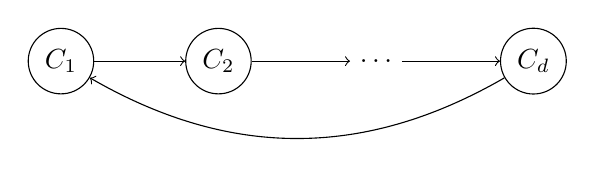
\begin{tikzpicture}[->,node distance=2cm]
        \node[circle, draw](c1){$C_1$};
        \node[circle,draw](c2)[right of=c1]{$C_2$};
        \node[](dots)[right of=c2]{$\ldots$};
        \node[circle,draw](cd)[right of=dots]{$C_d$};
        \path (c1) edge (c2);
        \path (c2) edge (dots);
        \path (dots) edge (cd);
        \path (cd) edge [bend left] (c1);
    \end{tikzpicture}
    \label{dperiod}
\end{figure}
\section{Monte-Carlo integration}
We are interested in evaluating 
\begin{equation*}
    \mu_f := \mathbb{E}_{\pi}  [f(X)] = \int_S f(x) \pi(dx)
\end{equation*}
as an integration problem.
If $S$ is discrete this takes a more familiar form $\sum_{i \in S}f(i)\pi_i$ \\
The problems can arise from the fact that$\pi$ can be multidimensional, and possibly unmormalized. Some example of these situations may be:
\begin{itemize}
    \item $f(x) = 1$ $\implies \mu_f$ is normalizing constant.
    \item If $f$ is the identity we are calculating the mean of $\pi$.
    \item If $f(x) = \mathbbm{1}_A(x) $ then tail probability and confidence intervals. 
\end{itemize}
We can also be interested in finding 
\begin{equation*}
    argmax_{x \in S} \pi (x) 
\end{equation*}
and this is an optimization problem, like for instance the mode of a distribution of interest. \\
Often an analytical computation is unfeasible and thus we need to use an approximation. Deterministic approximation include:
\begin{itemize}
    \item Riemann integration: given a partition of $S$ through points  $x_1, \dots, x_n$ then 
    \begin{equation*}
        \sum_{i=1}^n f(x_i) \pi (x_i) (x_i+x_{i-1}) \rightarrow \int f d\pi
    \end{equation*}
    as $sup_i |x_i+x_{i-1}| \rightarrow 0$.picture \\
    potentially ineficient especially in high dimention.
    \item Laplace approximation: use a Gaussian kernel to approximate a function of interest centered at the mode.
    \end{itemize}
    \begin{example}
       Let $f$ be unimodal:
    \begin{equation*}
        \int f (x) dx = \int e^{h(x)} dx 
    \end{equation*}
    take $h(x)= log f(x)$ and take a taylor of $h$ around the mode of $f$
    \begin{equation*}
        h(x)  \approx h (x_0) + \underbrace{h'(x_0)(x-x0)}_{f'/f|_{x_0}=0}+ 1/2h''(x_0)(x-x0) manca 
    \end{equation*}
    negative because we are at the mode
    \begin{equation*}
        \int f(x) dx \approx e ^{h(x_0)} \int  e ^{1/2 |h''(x_0)|(x-x0)} dx=
    \end{equation*}
    multiply and divide by $c:=\sqrt{2 \pi |h''(x_0)|^{-1}}$ and we have 
    \begin{equation*}
        =f(x_0) c \int \mathcal{N}(x; x_0, |h''(x_0)|^{-1})dx
    \end{equation*}
    this approximation is only good around the mode, but it loses a great part of its accuracy when we depart from the centre of the distribution: this makes it particularly bad for approximating, for instance, tails of a distribution. Moreover, if we work in high dimension more problems arise. $f$ needs to be unimodal, else this approach can fail (e.g. mixture models that came up a lot in statistics)     
    \end{example}

Deterministic approximations typically do not exploit information about the shape of the distribution of interest and this naturally leads to \enf{stochastic approximation}. 
\subsection{The Monte Carlo principle}
the main idea consists in exploiting information about $\pi$ and concentrate resources where they are most useful. From a general point of view simulate from $\pi$ and compute an approximation of the functional of interest. 

\begin{algorithm}{\enf{General strategy:}}
\begin{itemize}
    \item sample $X_1, \dots, X_n \stackrel{iid}{\sim}\pi$. \\
    ($N=$ MC sample size )
    \item $\mu_N = \frac{1}{N} \sum_{i=1}^N f(X_i) $\\
    \end{itemize}
    \end{algorithm}
    Note that if $\pi_N:= \frac{1}{N} \sum_{i=1}^N \delta_{X_i}$ then we have just 
    \begin{equation*}
        \mu_N = \int f(x) \pi_N (dx) = \frac{1}{N} \sum_{i=1}^N\int f(x)\delta_{X_i}  (dx) = \frac{1}{N} \sum_{i=1}^N f(X_i)
    \end{equation*}
    now 
    \[
    \mathbb{E}_\pi\left[\mu_N\right]=\frac{1}{N}\sum_{i=1}^{N}\mathbb{E}_\pi\left[f(x_i)\right]=\int f(x)\pi(dx)=\mu_f
    \]
    so $\mu_N$ is unbiased. Moreover, if $\mathbb{E}_\pi(f)<\infty$,
    \[
    \mu_N\xrightarrow{a.s.}\mu_f\qquad\text{by SLLN.}
    \]
    If $\mathbb{E}_{\pi} (f^2) < \infty$, set 
    \begin{equation*}
        \sigma_f ^2 := Var [f(X)] = \mathbb{E}_{\pi} [(f(X)- \mu_f)^2]
    \end{equation*}
    then $\mu_N$ has variance 
    \begin{equation*}
         \sigma_N ^2= Var(\mu_N) = \frac{\sigma_f ^2}{N}
    \end{equation*}
    so $\mu_N$ is a constant estimator of $\mu_f$. We also have a central limit theorem
    \begin{equation*}
         \sqrt{N} (\mu_N-\mu_f) \xrightarrow{d} \mathcal{N}(0, \sigma_f ^2)
    \end{equation*}
    to be used, e.g., for constructing asymptotic confidence intervals. 
Some potential issues are:
\begin{itemize}
    \item it may be computationally expensive;
    \item sampling directly from $\pi$ could be unfeasible and/or too difficult (e.g. high-dimensional distribution, distributions whose normalizing constant is unknown...).
\end{itemize}
    example. $Z \in \mathcal{N}(0,1)$. We are interested in 
    \begin{equation*}
        \mu= \mathbb{P}(Z> 5) = \int _{\mathbb{R}}\underbrace{\mathbbm{1}(x >5)}_{\mathclap{f(x)}} \varphi (z) dz
    \end{equation*}
    The value for $\mu$ is around $2.87\times10^{-7}$. Now draw $X_i \stackrel{i.i.d.}{\sim} \mathcal{N}(0,1)$
    \begin{equation*}
        \mu_N = \frac{1}{N} \sum_{i=1}^N \mathbbm{1}(x_i >5) \rightarrow \mu
    \end{equation*}
    This means that as long as we draw $N<\mathcal{O}(10^7)$ we expect to see a positive indicator... 0 times. This is an example of situation where simulating $\pi$ is computationally infeasible. To face this limitation, we turn to a very important idea: the \textbf{rejection sampling}. 
\subsection{Rejection Sampling}
\begin{algorithm}
    until $N$ points are saved repeat:
    \begin{itemize}
        \item draw independently $Z \sim Unif (a,b)$ and $ Y \sim Unif(0,M) $;
        \item if $y \leq \pi(z)$, set $X=z$.
    \end{itemize}
\end{algorithm}
\begin{figure}[H]
\centering
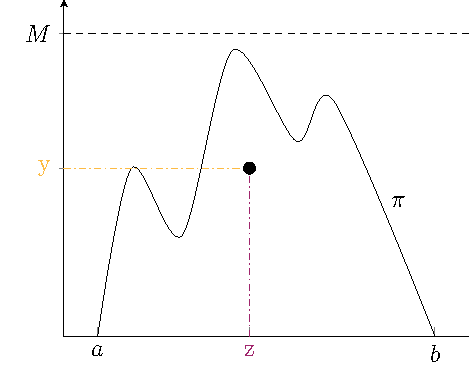
\includegraphics{standalones/pdfs/rejection1}
    \label{rejsampl}
\end{figure}
Only points under $\pi $ are kept, and these are draws from $\pi$. Cdf of accepted points:
\begin{equation*}
\begin{split}
    \mathbb{P}(Z \leq x| Y \leq \pi(Z))&= \frac{\mathbb{P}(Z \leq x, Y \leq \pi(Z))}{\mathbb{P}( Y \leq \pi(Z))}\\
    &= \frac{\mathbb{P}(Z \leq x, Y \leq \pi(Z))}{\mathbb{P}( Z \leq b, Y \leq \pi(Z))}\\
    &= \frac{\int_a^x \int_0 ^{\pi(Z)}\frac{1}{M}dy \frac{1}{b-a}dz} {\int_a^b \int_0 ^{\pi(Z)}\frac{1}{M}dy \frac{1}{b-a}dz}\\
    &= \int_a^x \pi(Z) dz
\end{split}
\end{equation*}
so now we can compute  $\mu_N = \frac{1}{N} \sum_{i=1}^N f(X_i) $. 

If the support of $\pi$ is unbounded, we cannot draw from $Unif(a,b)$, the idea is that we are gonna use a non uniform bound and an auxiliary distribution. \\
Assume:
\begin{itemize}
    \item $\exists M>0$ and a density $q$ such that
    \begin{equation*}
        \pi (x) \leq Mq(x)
    \end{equation*}
    \item we can draw from $q$, meaning that we should choose a $q$ we can simulate relatively easily.
\end{itemize}
\begin{algorithm}
    until $N$ points are saved:
\begin{itemize}
    \item draw $Z\sim q$, with $Y|Z=z\sim Unif(0, Mq(z))$;
    \item if $Z\leqslant\pi(z)$, set $x=Z$.
\end{itemize}
\end{algorithm}
\begin{figure}[H]
\centering
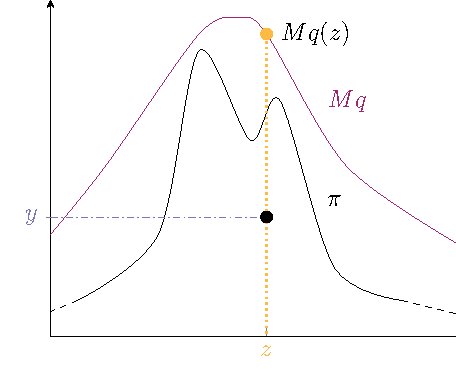
\includegraphics{standalones/pdfs/rejection2}
    \label{res2}
\end{figure}
Verify $(-\infty\leqslant a < b \leqslant\infty)$=\[
=\dfrac{\displaystyle\int_{-\infty}^{x}\int_0^{\pi(z)}\frac{1}{\cancel{Mq(z)}}dy\,\cancel{q(z)}dz}{\displaystyle\int_{-\infty}^{\textcolor{red}{\infty}}\int_0^{\pi(z)}\frac{1}{\cancel{Mq(z)}}dy\,\cancel{q(z)}dz}=\mathbb{P}(X\leqslant x)\
\]
\begin{example}
    take $\mu=\mathbb{P}(z>5)=2.87\cdot10^{-7}$. We need a non-uniform bound:
\[
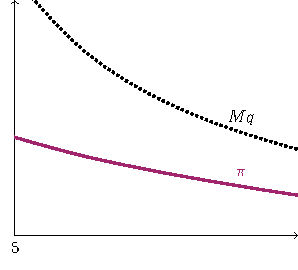
\includegraphics{standalones/pdfs/normsampl}
\]
Choose $q(x)=e^{-(x-5)}\mathbbm{1}(x>5)$ with $M=\phi(5)$. We know that
\[\mu_N=\% \text{ of accepted points}\times\underbrace{\text{area of graph where we generate values}}_{\int_5^\infty Mq(x)dx=M\int_5^\infty e^{-(x-5)}d=M}\]
This algorithm is generally more efficient than naive Monte-Carlo where we would have to generate $x_i\sim N(0,1)$ variables and keep $x_i>5$. It can be, anyway, costly: the acceptance probability over an interval $(c,d)$ is
\begin{align*}
    \mathbb{P}(c\leqslant Z\leqslant d, Y\leqslant\pi(z))&=\int_c^d\int_0^{\pi(z)}\frac{dy}{Mq(z)}q(z)dz\\
    &=\frac{1}{M}\int_c^d\pi(z)dz.
\end{align*}
In general, over the support, the acceptance probability is $\frac{1}{N}$. So, in order to have $N$ points, we need to generate a number of points equal to
\[N'\sim Neg-Bin\Bigl(N,\frac{1}{M}\Bigr).\]
\[\frac{1}{M}\int_5^\infty\pi(x)dx=\frac{2.87\cdot10^{-7}}{1.49\cdot10^{-6}}=0.19\]
\end{example}
\subsection{Importance Sampling}
This idea starts with a little analytical trick, in general terms the idea is to use all generated samples. Unlike the accept-reject method. \\
\begin{equation*}
\begin{split}
    \mu&= \mathbb{E}_{\pi}[f(x)] = \int f(x) \pi(x) dx = \int f(x) \frac{\pi(x)}{q(x)} q(x) dx \\
    &= \mathbb{E}_{q}[f(x)\frac{\pi(x)}{q(x)}]
\end{split}
\end{equation*}
where $q$ is a density whose support include that of $\pi$.\\ (i.e. $q(x)=0$ $\implies$ $\pi(x)=0$)\\
Then we can:
\begin{itemize}
    \item draw $X_i \stackrel{\text{i.i.d.}}{\sim} q$ 
    \item assign weight $w(x_i):= \frac{\pi(X_i)}{q(X_ i)}$ to $X_i$. ($w$ importance weight)
    \item  set 
    \begin{equation*}
        \mu_N= \frac{1}{N} \sum_{i=1}^N f(X_i)w(X_i)
    \end{equation*}
\end{itemize}
Then
\begin{equation*}
    \mathbb{E}_q[\mu_N]= \mathbb{E}_q [f(x)w(x)] \stackrel{above}{=} \mu 
\end{equation*}
moreover
\begin{equation*}
    \mu_N \xrightarrow{a.s.} \mu \hspace{0.5 cm} \text{ as } n \rightarrow + \infty
\end{equation*}
\begin{figure}[H]
    \centering
    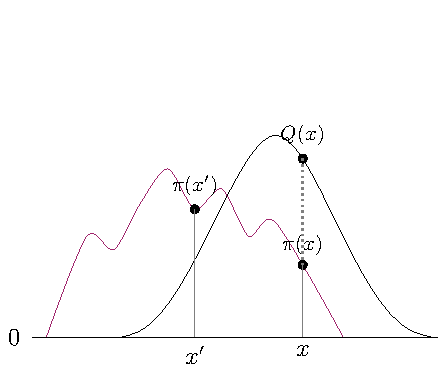
\includegraphics{standalones/pdfs/impsamp}
    \label{impsamp}
\end{figure}
\begin{itemize}
    \item down-weight importance of $x$\\
    $\pi (x) < q(x) \implies w(x) = \frac{\pi (x)}{q(x)}< 1$. 
    \item $w(x')>1$ up-weight of $x'$.
\end{itemize}
draws in relevant regions are up-weighed automatically and no draws are wasted. The choice of $q$ is more flexible than in the AR method.\\ 
\textbf{Toy Example.} $\mathbb{P}(Z>5) = \mu= 2.87 \times 10 ^{-7}$\\\
Use 
\begin{equation*}
    q(x)= e ^{-(x-5)} \mathbbm{1}_{\{x>5\}},
\end{equation*}
and so 
\begin{equation*}
    \mu = \int_5^{\infty} \phi(x) dx= \int_{\mathbb{R}} \mathbbm{1}_{\{x>5\}} \phi(x) dx = \int_{\mathbb{R}} \underbrace{\mathbbm{1}_{\{x>5\}}}_{= f(x)} \underbrace{\frac{\phi(x)}{q(x)}}_{=w(x)} q(x) dx
\end{equation*}
so $X_i \stackrel{\text{i.i.d.}}{\sim} q $.
\begin{equation*}
    \mu_N= \frac{1}{N} \sum_{i=1}^N f(X_i)w(X_i) = \frac{1}{N} \sum_{i=1}^N \underbrace{\mathbbm{1}_{X_i>5} }_{\text{since } X_i \sim q }\frac{\phi(x_i)}{q(x_i)}  = \frac{1}{N} \sum_{i=1}^N\frac{\phi(x_i)}{q(x_i)} 
\end{equation*}
Additional upside:\\
if $\pi= \frac{\tilde{\pi}}{z}$ with $z$ unknown. Then
\begin{equation*}
    \mu = \int f(x) \pi (x) dx = \int f(x)\frac{\tilde{\pi(x)}}{z q(x)} q(x) dx 
\end{equation*}
\begin{equation*}
    \rightarrow \ \ z= \int \tilde{\pi(x)} dx = \int \frac{\tilde{\pi(x)}}{q(x)}q(x) dx 
\end{equation*}
so setting $\tilde{w}(x)=\frac{\tilde{\pi(x)}}{q(x)}$ we have 
\begin{equation*}
     \mu = \underbrace{\frac{\int f(x) \Tilde{w}(x) q(x) dx }{\int \Tilde{w}(x) q(x) dx}}_{\text{self-normalizing estimate}}
\end{equation*}
Hence for $X_i \stackrel{\text{i.i.d.}}{\sim} q $ we now have 
\begin{equation*}
    \Tilde{\mu}_N = \frac{\frac{1}{N} \sum_{i=1}^N f(X_i)\Tilde{w}(X_i)}{\frac{1}{N} \sum_{j=1}^N \Tilde{w}(X_j)} = \sum_{i=1}^N  f(X_i) \hat{w}(X_i)
\end{equation*}
with $\hat{w}(X_i)= \frac{\Tilde{w}(X_i)}{\sum_{j=1}^N \Tilde{w}(X_j)}$. Strong law of large numbers still applies. \\
\subsection{Markov-Chain Monte-Carlo}
When:
\begin{itemize}
    \item Tails of $q$ versus $\pi$ can be very different so that $w(x)$ possibly unbounded
    \item $q$ may be difficult to identify in high-dimensions
\end{itemize}
Idea: we can generate draws from $\pi$ using Markov Chains, obtaining what is called \textbf{Markov Chains Monte Carlo}.\\
Given a target distribution $\pi$, we want to construct an ergodic Markov chain $X$ with stationary distribution $\pi$, and use its trajectory to get draws from $\pi$. \\
Assume for now $P$ is ergodic. \\ Given an intial state $X_0$, we can in principal simulate trajectory :\\
$\forall \ n \geq 0 $, if $X_n = i$, draw $X_{n+1}=j$ with probability $p_{ij}$
from ergodicity we know 
\begin{equation*}
    \exists n_0 \in \mathbb{N}: X_n \sim \pi \ \ \forall n \geq n_0
\end{equation*}
Such $n_0$ is called Mixing time, meant as an order of magnitude, not as a step. (e.g. $n_0=O(10^4)$)\\
Studying mixing times is typically difficult. Usually one uses convergence test or diagnostics.
(there is literature, Gelman-Rubin criterion).\\
Suppose we know $n_0$. Then 
\begin{itemize}
    \item simulate $\{X_n ^{(i)}, n \leq n_0\}$ for $i=1, \dots, N$.
    \item set $Y_i = X_{n_0+i}$ (sample path endpoint).
\end{itemize}
Then $(Y_i, \dots, Y_N)$ is the MCMC sample. These are i.i.d $\sim \pi$ (assume $X_0^{(i)}$ independent).\\
$\implies$ we are back t0 the Monte-Carlo scenario with 
\begin{equation*}
    \mu_N = \frac{1}{N}\sum_{i=1}^N f(Y_i) \xrightarrow{a.s.} \mu_f
\end{equation*}
where 
\begin{equation*}
    Var(\mu_N)= \frac{\sigma_f^2}{N}, \  \  \ \sigma_f^2= Var_{\pi}(f(Y)). 
\end{equation*}
However we are discarding  $N=n_0$ sample. If, for example, $N= 10^4$, $n_0= 10^5$ $\implies 10^9$, which is expensive.\\
alternatively, we can think of using a single chain . \\
\begin{algorithm}[\textbf{Generic MCMC strategy}]
   Given $N$:
\begin{itemize}
    \item simulate $\{X_n, n\}$
    \item  for $n_0$ large enough, set 
    \begin{equation*}
        \hat{Y}_i= X_{n_0+i}, \ \ i = 1,\dots,N 
    \end{equation*}
\end{itemize}
\begin{equation*}
    \implies \mu_N = \frac{1}{N}\sum_{i=1}^N f(\hat{Y}_i)\approx \mu_f 
\end{equation*} 
\end{algorithm}

\begin{figure}[H]
    \centering
    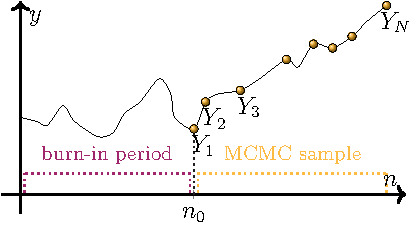
\includegraphics{standalones/pdfs/burnin}
\label{burnin}
\end{figure}
Only $n_0$ values wasted. %it's a strong statement man. 
The MCMC samples are now correlated and the MCMC estimator is now no longer a generic sample average but it is an ergodic average. In terms of theoretical result we have the ergodic theorem that guarantees 
\begin{equation*}
    \frac{1}{N}\sum_{i=1}^N f(\hat{Y}_i) \xrightarrow{a.s.} \mu_f = \mathbb{E}_{\pi}[f(Y)]
\end{equation*}
for any initial distribution.\\ Understand what we are losing, consider the variance of $\hat{\mu}_N$ 
\begin{equation*}
    Var\Bigg(\frac{1}{N}\sum_{i=1}^N f(\hat{y}_i)\Bigg) = \frac{1}{N^2}\sum_{i=1}^N\Bigg[Var\Big(f(\hat{y}_i)\Big)+2\sum_{k=1}^{N-1}Cov\Big(\underbrace{f(\hat{y}_i,f(\hat{y}_{i+k})}_{\mathclap{\text{autocovariance function}}}\Big)\Bigg]
\end{equation*}
at equilibrium, $Var$ and $Cov$ do not depend on time but only on the lag.  In particular $Var(f(\hat{Y}_i))= \sigma_f^2$. 
\begin{equation*}
    %Ha ripreso la roba di prima
    \frac{1}{N^2}  \sum_{i=1}^N \left[\sigma_f^2 + 2 \sigma_f^2\underbracket{\sum_{k=1}^{N-i}\frac{Cov(f(\hat{Y}_i),f(\hat{Y}_{i+k} )}{\sigma_f^2}}_{\mathclap{\gamma_k=Corr\left(f(\hat{y}_i,f(\hat{y}_{i+k})\right)}}\right] \approx \frac{\sigma_f^2}{N}(1+\sum_{k\geq 1}\gamma_k)
\end{equation*}
This is higher the the variance of the MCMC estimator with $N$ chains (in fact it is a MC estimator). The quantity 
\begin{equation*}
    \Tilde{N} = \frac{N}{1 +2\sum_{k\geq 1}\gamma_k }
\end{equation*}
is called \textbf{effective sample size}. Indeed

\begin{align*}
       &\frac{Var(\hat{\mu}_N)}{Var(\mu_N)} = \frac{\sigma_f^2/\Tilde{N}}{\sigma_f^2/N} \\
    \implies &ESS= N \frac{Var(\hat{\mu}_N)}{Var(\mu_N)}  \in [0,N] 
\end{align*}

so the $ESS$ reppresent the size of an iid smaple with the same variance of the MCMC sample, giving a measure of the loss of efficiency determined by using a correlated sample. \\
Here we are hoping $\gamma_k$ decays fast. Other wise the common practice is to perform what is called thinning, that is setting 
\begin{equation*}
    \hat{Y}_i = X_{n_0+ih } \hspace{0.5 cm} i = 1, \dots, N
\end{equation*}
for a chosen $h \in \mathbb{N}$. This lowering the correlation among succesive samples. \\
In fact debated practice 
\begin{itemize}
    \item now we discard a higher number of samples.
    \item it is belived that keeping all sample after the burn-in yield's a better approximation of $\mu_f$.
\end{itemize}
Observation even if are correlated are pieces of information so don't waste them, on the other hand maybe you want to remove correlation. 
\subsection{Metropolis-Hastings algorithm}
The \textbf{Metropolis-Hastings algorithm} has been selected among the 10 most important algorithms of the 20th century. 

The idea consists in running a chain with arbitrary transition matrix, but sometimes suppressing transition (in a "right way"). Given a target $\pi$ on $S$, let:
\begin{itemize}
    \item [-]$Q$ be an aribtrary, irreducible transition matrix called \textit{proposal matrix};
    \item [-]$A$ be a matrix with entries $a_{ij}\in[0,1]$ called \textit{acceptance matrix}.
\end{itemize}
\begin{algorithm}[\textbf{Generic Metropolis-Hastings}]
    For $n\geqslant 1$, if $X_{n-1}=i$:
    \begin{itemize}
        \item [-] draw $j$ with probability $q_{ij}$;
        \item [-] set $X_n=j$ with probability $a_{ij}$; else set $X_n=X_{n-1}$
    \end{itemize}
\end{algorithm}
$Q$ provides proposal states: from row $i$ draw state $j$, $A$ tells us if we should go in $j$ or stay where we are. The resulting transitions are:
\[
p_{ij}=\begin{cases}
    q_{ij}a_{ij} &j\neq i\\
    1-\sum_{k\in S}  q_{ik}a_{ik} &j=i.
\end{cases}
\]
\begin{itemize}
    \item[$\rightarrow$]$Q=(q_{ij})_{i,j}\in S$ is aribtrary (which means we can choose a distribution easy to simulate from);
    \item[$\rightarrow$]$P=(p_{ij})_{i,j\in S}$ is irreducible since $Q$ is aperiodic and since $X_n=X_{n-1}$ with positive probability.
\end{itemize}
So if we show $P$ has invariant distribution $\pi$, then it is positive recurrent and the ergodic theorem applies: $\pi$ is therefore also the equilibrium distribution. \\
Idea: occasionally suppress transitions to state that are less likely "with respect to $\pi$", so to speak.
\begin{proposition}
    The Metropolis Hastings algirthm with proposal matrix $Q$ and acceptance probabilities
        \[
        a_{ij}=\min\bigg\{1,\frac{\pi_jq_{ji}}{\pi_iq_{ij}}\bigg\}
        \]
        generates a \textbf{reversible chain} with respect to $\pi$.
\end{proposition}
\begin{proof2}
    We need to show that $\pi_ip_{ij}=\pi_jp_{ji}$ (detailed balance for the resulting chain).
        \begin{align*}
            \pi_ip_{ij}&=\pi_iq_{ij}a_{ij}\\
            &=\pi_iq_{ij}\min\bigg\{1,\frac{\pi_jq_{ji}}{\pi_iq_{ij}}\bigg\}=\\
            &=min\bigg\{\pi_iq_{ij},\pi_jq_{ji}\bigg\}.
        \end{align*}
        But since minimum is symmetric and \[
        min\big\{\pi_jq_{ji},\pi_iq_{ij}\big\}=min\big\{\pi_iq_{ij},\pi_jq_{j1}\big\}.
        \]
        starting from $\pi_jq_{ji}$ yields the same term, so $\pi_i p_{ij}=\pi_jp_{ji}$.
\end{proof2}
\begin{algorithm}\enf{Metropolis-Hastings Algorithm}
     For $n\geqslant1$, if $X_{n-1}=i$:
    \begin{itemize}
        \item [-] draw $J=j$ with probability $q_{ij}$;
        \item [-] draw $U\sim Unif(0,1)$;
        \item [-] if $U<\min\left\{1,\frac{\pi_jq_{ji}}{\pi_iq_{ij}}\right\}$ set $X_n=j$; else $X_n=X_{n-1}$
    \end{itemize}
\end{algorithm}
This algorithm has important features:
\begin{itemize}
    \item the proposal distribution is fully arbitrary, with the sole condition of being irreducible. This leaves us a lot of freedom.
    \item it applies even if the normalizing constant of $pi$ is unknown, since
    \[
    \frac{\pi_j}{\pi_i}=\frac{\tilde{\pi}_j/\cancel{z}}{\tilde{\pi}_i/\cancel{z}}=\frac{\tilde{\pi}_j}{\tilde{\pi}_i}
    \]
\end{itemize}
\begin{example}
    \[
\pi(\cdot)=cPois(\cdot;\lambda_1)+(1-c)Pois(\cdot;\lambda_2)
\]
is a mixture of Poisson distributions. We want to reconstruct this target using ergodic average. Propose states with a simple MC: we will use a $B\&D\left(\frac{1}{2},\frac{1}{2}\right)$ (i.e. a symmetric random walk on $\Z_+$).
\begin{align*}
    \implies &q_{ij}=\frac{1}{2}\qquad\text{for }j=(i\pm1)^+\\
    & a_{ij}=\min\{1,\alpha_{ij}\}\qquad\alpha_{ij}=\frac{\pi_jq_{ji}}{\pi_iq_{ij}}\\
    \implies &\alpha_{ij}=\frac{cPois(j;\lambda_1)+(1-c)Pois(j;\lambda_2)}{cPois(i;\lambda_1)+(1-c)Pois(i;\lambda_2)}\cdot\frac{\cancel{1/2}}{\cancel{1/2}}
\end{align*} This last equality is true for $j=(i\pm1)^+$ and arbitrary for all other $j$s, which are not going to be proposed wince we use a random variable. The code can be found in appendix. %\ref{poiscode}.
The random walk is not positive recurrent, but Metropolis-Hastings "corrects" the trajectory so that it basically becomes recurrent.
\end{example}
The previous example refers to a typical class of Metropolis-Hastings algorithms called \textit{random walk Metropolis-Hastings}, where
\[
X_n=X_{n-1}+Z_n
\]
Where $Z_n$ has symmetric distribution around zero. The example provided, in particular, is a special case called \textbf{Metropolis} algorithm, where the proposal is symmetric so that
\[
q_{ij}=q_{ji}\implies a_{ij}=\min\left\{1,\frac{\pi_j}{\pi_i}\right\}.
\]
So:
\begin{itemize}
    \item if $\pi_j<\pi_i$ we accept the step with probability $<0$;
    \item if $\pi_j>\pi_i$ we accept the step with probability 1.
\end{itemize}

We can interpret this consequence of the algorithm as the fact that if the density of the new step increases, we accept the step and we continue exploring that direction; otherwise, we still have a chance to accept the new steps even if it leads us to a zone with lower density. Of course, if we only accepted steps that increase the density we would basically have an optimization algorithm that maximizes probability density (which is not what we want).
\begin{example}
    \[
\pi(\cdot)=cN(\cdot;\mu_1,\sigma_1^2)+(1-c)N(\cdot;\mu_2,\sigma_2^2).
\]
We can use a random walk Metropolis-Hastings that proposes
\[
Y=X+Z\qquad Z\sim N(0,\sigma_0^2)
\]
if $X_{n-1}=X$, and $\alpha_{ij}$ is now
\[
\alpha(x,y)=\frac{\pi(y)q(x|y)}{\pi(x)q(y|x)}
\]
where $q(y|x)=N(y;x,\sigma_0^2)$. They are symmetric, so
\[
\alpha(x,y)=\frac{\pi(y)}{\pi(x)}
\]
\end{example}
Another special case is the \textit{independent Metropolis-Hastings}, where the proposal does not depend on the current state, i.e.
\[
q_{ij}=q_j\implies a_{ij}=\min\left\{1,\frac{\pi_jq_i}{\pi_iq_j}\right\}=\min\left\{1,\frac{\pi_j/q_j}{\pi_i/q_i}\right\}.
\]
Proposals are accepted with probability 1 if
\[
w_j=\frac{\pi_j}{\pi_j}>\frac{\pi_i}{\pi_i}=w_i\qquad\text{(it's a reweighing)}
\]
Analogies:
\begin{itemize}
    \item with \textit{importance sampling}: $w(x)=\frac{\pi(x)}{q(x)}$ is the importance weight, i.e. we accept with probability 1 if $w_j>w_i$ (which means there has been an improvement in importance weights).
    \item with \textit{rejection sampling}: propose $z=j$ with probability $q_j$ and accept if $y\leqslant\pi_j$ where $y|z=j\sim Unif(0,Mq)$ which is the same as \[
    U<\frac{\pi_j}{Mq_j},\qquad U\sim Unif(0,1)
    \]
    that here becomes $U<\frac{\pi_j/q_j}{\pi_i/q_i}$ instead of $\frac{\pi_j}{Mq_j}$.
\end{itemize}
\subsection{Gibbs sampling}
Gibbs sampling is formally a special case of Metropolis-Hastings but it found wider applications. It is useful with:
\begin{itemize}
    \item multivariate $\pi$;
    \item models with latent variables;
    \item models specified using conditionals.
\end{itemize}
Gibbs sampling needs at least a bivariate space. Let $\pi=\pi_{X,Y}$ density on $S\times S$. We cannot sample directly from $\pi$ but we can sample from the conditionals $\pi_{X|Y}$ and $\pi_{Y|X}$.
\begin{algorithm}[\textbf{Two-component Gibbs sampler}]
    Given $(X_{n-1},Y_{n-1})=(x,y)$ as our current state,
    \begin{itemize}
        \item [-] draw $X'\sim\pi_{X|Y}(\cdot|Y)$ 
        \item [-] draw $Y'\sim\pi_{X|Y}(\cdot|X)$
        \item [-] set $(X_n,Y_n)=(X',Y')$
    \end{itemize}
\end{algorithm}
Why is this useful? If $(X,Y)\sim\pi_{x,y}$ this is equivalent to say that
\[
Y\sim \pi_y \;\text{(marginal distribution)},\quad X|Y\sim\pi_{X|Y}\;\text{(chain rule)}
\]
but if $X'\sim \pi_{X|Y}$ then 
\[
(X',Y)\sim\pi_{X,Y}
\]
which is obvious, since we drew it that way. The same holds for $Y'$, so these transitions preserve the joint distribution $\pi_{X,Y}$ which is therefore invariant.
\begin{proof2}
 The first step of the algorithm can be seen as a Metropolis-Hastings step with proposal on $S^2=S\times S$:
        \[
        q=(X',Y'|X,Y)=\pi_{X'|Y'}(X'|y)\mathbbm{1}(Y'=y).
        \]
        In practice, we fix $Y$ and then we update $X$. The acceptance rate is $\min\left\{1,\frac{\pi_jq_{ji}}{\pi_iq_{ij}}\right\}$. If we factorize in marginals and conditional we get:
        \[
        \frac{\textcolor{red}{\pi(X'Y')}\textcolor{blue}{q(X,Y|X',Y')}}{\textcolor{Dandelion}{\pi(X,Y)}\textcolor{OliveGreen}{q(X',Y'|X,Y)}}=\frac{\textcolor{red}{\pi(Y')\pi(X'|Y')}\textcolor{blue}{\pi(X|Y')\mathbbm{1}(Y=Y')}}{\textcolor{Dandelion}{\pi(Y)\pi(X|Y)}\textcolor{OliveGreen}{\pi(X'|Y)\mathbbm{1}(Y=Y')}}
        \]
        but since we imposed $Y=Y'$, all these factors cancel out:\[
        =\frac{\textcolor{red}{\cancel{\pi(Y')\pi(X'|Y')}}\textcolor{blue}{\cancel{\pi(X|Y')}\cancel{\mathbbm{1}(Y=Y')}}}{\textcolor{Dandelion}{\cancel{\pi(Y)\pi(X|Y)}}\textcolor{OliveGreen}{\cancel{\pi(X'|Y)}\cancel{\mathbbm{1}(Y=Y')}}}=1.\]
\end{proof2}
So every step of the Gibbs samples is made of 2 mini Metropolis-Hastings steps with probability of acceptance 1: we never reject any data. If we are only interested in $X$ univeriates we can sometimes augment the state space to $S\times S'$ through can auxiliary variable $Y\in S'$ paradoxally introduced to ease the computation. The transition for $X$ (marginal) can be written, integrating $Y$ out, as \[
p_X(x'|X)=\int_{S'}\pi_{Y|X}(y|x)\pi_{X|Y}(x'|y)dy.
\]
Stationarity requires, by the global balance conditions:
\[
\int_S\pi_X(x)p_X(x'|X)dx=\pi_X(x').
\]
We have
\[
\int_{S}\pi_{X}(x)p_X(x'|X)dx=\int_S\pi_X(x)\left(\int_{S'}\pi_{Y|X}(y|X)\pi_{X|Y}(x'|Y))dx\right)dy.
\]
Using Fubini's theorem
\begin{align*}
&\int_{S'} \pi_{X|Y}(x'|Y)\int_S\underbracket{\pi_{Y|X}(y|X)\pi_X(X)}_{\pi_{X,Y}(X'Y)}dxdy\\
&\int_S \underbracket{\pi_{X|Y}(x'|Y)\pi_{Y}(y)}_{\pi_{X,Y}(X',Y)}dy=\pi_X(x')
\end{align*}
A Gibbs sampler on $(X_n,Y_n)$ yields, marginally, a stationary $X_n$ chain with respect to $\pi_X$.
If we are interested in $X$, $Y$ can be sometimes an auxiliary variable: \\
\begin{itemize}
    \item we run the Gibbs sampler on $(X_n, Y_n)$
    \item discard $Y_n$
    \begin{equation*}
    \begin{split}
        \implies \ \ X_n (\text{ at stationarity })\\
        \text{is from }\pi_x = \int \pi_{X,Y}(x,y)dy
    \end{split}
    \end{equation*}
\end{itemize}
\begin{example}
    In a popular Bayesian model we have 
\begin{equation*}
    \pi_X (x) \propto x ^{\alpha+k-1} e ^{-\beta x} \frac{\Gamma(x)}{\Gamma(x+n)}, \hspace{0.5 cm } x \geqslant 0.
\end{equation*}
Normalizing and simulating from $\pi$ is not trivial, due to the presence of gamma functions. However, 
\begin{equation*}
    \frac{\Gamma(x)\Gamma(n)}{\Gamma(x+n)}=\int_0^1 y^{x-1}(1-y)^{n-1}\dif y
\end{equation*}
so we can formulate a joint model on the augmented state space $\mathbb{R}_+ \times [0,1]$.
\begin{align*}
    \pi_{X,Y}(x,y)&\propto x ^{\alpha+k-1} e ^{-\beta x}\overbracket{y^{x-1}(1-y)^{n-1}}^{\text{Beta kernel}}\\
    &\implies\int_0^1 \pi_{X,Y}(x,y)\dif y=\pi_X(x)
\end{align*}
So we have 
\begin{itemize}
    \item for fixed $x$, $\pi(y|x)= Beta(x,n) $
    \item  for fixed $y$,
    \begin{align*}
        \pi (x|y) &\propto x ^{\alpha+k-1} x ^{\alpha+k-1} e ^{-\beta x} \underbrace{e ^{\ln(y^x)}}_{\mathclap{= y^x}}\\
        &= \underbracket{x ^{\alpha+k-1} e ^{-(\beta x -\ln y)x}.}_{\mathclap{x^ae^{-bx}\text{: Gamma distribution, once we fix }y}}
    \end{align*}
    So the Gibbs sampler runs 
    \begin{itemize}
        \item $X|Y \sim Gamma(\alpha+k, \beta- \ln y)$
        \item $Y|X \sim Beta(x,n)$
    \end{itemize}
    and the just discards discard the value of $Y$.
\end{itemize}
\end{example}
More generally, let $\pi (x)= \pi(x_1, \dots, x_d)$ be a density on $S^d$, $d \geqslant 2$. \\
Denote $x_{(-i)}=(x_1, \dots,x_{i-1}, x_{i+1}, \dots,  x_d) $. Assume we know how to sample from the full conditional distributions 
\begin{equation*}
    \pi(x_i |x_{(-i)})
\end{equation*}
The $i^{th}$ component Gibbs sampler updates $X_i$ and leaves the other coordinates unchanged, so 
\[
\begin{rcases*}
    (X_1,\ldots,X_i,\ldots,X_d)\sim\pi\\
    X_i'\sim\pi(x_i |x_{(-i)})
\end{rcases*}\implies (X_i,\ldots,X_i',\ldots,X_d)\sim\pi.
\]
So $\pi$ is invariant and this is a Metropolis-Hastings step with proposal 
\begin{equation*}
    q(x'|x) = \pi ((x_i |x_{(-i)}) \mathbbm{1}(x'_{(-i)}= x_{(-i)})
\end{equation*}
and the acceptance probability is $1$.

The full Gibbs Sampler typically reads:
\begin{algorithm}[\textbf{Random Scan Gibbs Sampler}]
Given $X_n = x \in S^d$:
\begin{itemize}
    \item draw $i$ with probability $p_i $ ($\sum^d p_i = 1 $);
    \item draw $X_i'\sim \pi_{X_i|X_{(-i)}}(\cdot|x_{(-i)} )$;
    \item set $X_{n+1}=(x_1, \dots, x_{i-1},  x_{i-1}, x_{i+1}, \dots, x_d )$.
\end{itemize}
\end{algorithm}
If $p_i >0$ for all $i=1, \dots, d$, this algorithm produces a reversible chain with respect to $\pi$. This Gibbs sampling is so powerful that the cases in which we should \textit{not} use it are very specific. 
\subsection{Slice sampler}
Let $\pi_X$ be a density on $S$.
\begin{lemma}\label{slizer}
    Let $A$ be the area under $\pi_x$, i.e. 
    \begin{equation*}
        A= \{(x,y) \in S \times \mathbb{R}_+: 0 \leqslant y\leqslant \pi_X(x)\}
    \end{equation*}
    If $(X,Y)$ has uniform distribution on $A$, then $X \sim \pi_x $
\end{lemma}
\[
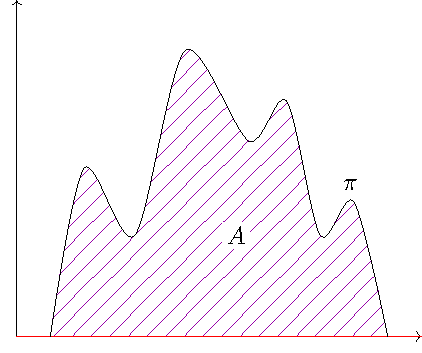
\includegraphics{standalones/pdfs/areaunder}
\]
\begin{proof2}
    If (X,Y) is uniform on A we have $\pi_{X,Y}(x,y)\propto\mathbbm{1}_{0\leqslant y\leqslant\pi(x)}$ whose normalizing constant is
    \[
    \int_S\int_0^\infty\mathbbm{1}_{0\leqslant y\leqslant\pi(x)}\dif y \dif x =\ldots=1.\]
    Then the marginal of $X$ is
    \begin{align*}
        \int_0^\infty \pi_{X,Y}(x,y) \dif y&= \int_o^\infty \mathbbm{1}_{0\leqslant y\leqslant\pi(x)}\dif y\\
        &=\int_0^{\pi_X(x)}\dif y=\pi_X(x)
    \end{align*}
   \end{proof2}
   AR methods are based on this result. 
     How does this connect with Markov-Chain Monte-Carlo? The main idea is that we can use  a Markov Chain whose equilibrium distribution is a uniform on $A$, then discarded $Y$ and keep $X$. The target is \[\pi_{X|Y}(x,y) \alpha 1_{0 \leqslant y \leqslant \pi(x)} \] and we need to construct a Markov Chain that is ergodic with respect to this target.  We can think a Gibbs sampler that alternate the draws from the two condition:
    \begin{itemize}
        \item $Y'|X\sim \pi_{Y|X}(y|x)\propto\mathbbm{1}_{0\leqslant y\leqslant\pi(x)}$ ($x$ is fixed: this step sets the height of the \textit{vertical slice});
        \item $X'|Y\sim \pi_{X|Y}(x|y)\propto\mathbbm{1}_{0\leqslant y\leqslant\pi(x)}$ ($y$ is fixed: this step sets the length of the \textit{horizontal slice}).
    \end{itemize}
    \begin{figure}[H]
        \centering
        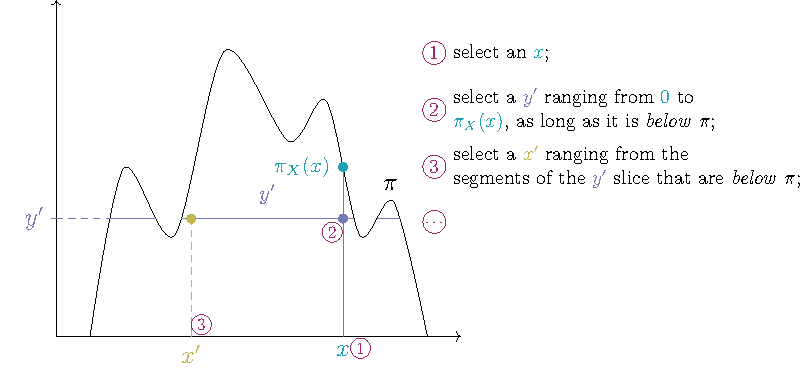
\includegraphics{standalones/pdfs/slicesampler}
        \label{slicesampler}
    \end{figure}
So these are reversible step with respect to $\pi_{X,Y}$ and at equilibrium we have uniform sample on A: then using the lemma \ref{slizer}, $X$ is from $\pi_X$.
\begin{example}

$S=\mathbb{R}_+, \hspace{0.5 cm} \pi(x)=\frac{1}{2}e^{-\sqrt{x}}, x > 0$.
\begin{equation*}
    \pi^{-1}(y) = (\log2y)^2
\end{equation*}
so the slice sampler is 
\begin{itemize}
    \item $Y'|x \sim$ Unif $(0,\frac{1}{2}e^{-\sqrt{x}} )$
    \item $X'|y' \sim$ Unif $(0,(\log2y))^2$
\end{itemize}

$\pi(x) \propto e^{-\sqrt{x}}, x \in \mathbb{Z}_+$ unnormalized.
\begin{equation*}
    \pi^{-1}(y) = (\log(y))^2
\end{equation*}
\begin{itemize}
    \item $Y'|x \sim$ Unif $(0,e^{-\sqrt{x}} )$
    \item $X'|y' \sim$ Unif$(\{0,1,\ldots, \lfloor{(\log(y))^2 \rfloor}\})$ 
\end{itemize}
Remember that 
\begin{equation*}
    \left \lceil{x}\right \rceil =\max \{n \geqslant 0: n \leqslant x\}
\end{equation*}
If $\pi$ is d-dimensional, it is typically difficult to identify
\begin{equation*}
    A_y = \{x: y \leqslant \pi(x)\}
\end{equation*}
If we can write 
\begin{equation*}
    \pi(x) \propto \prod_{i = 1}^d \pi_i(x)
\end{equation*}
we can use $d$ auxiliary variables $y_1, \ldots, y_d$, so that 
\begin{equation*}
    \pi_i(x) = \int_0^{\pi_i(x)}\dif y_i = \int \mathbbm{1}_{0 \leqslant y_i \leqslant \pi_i(x)} \dif y_i
\end{equation*}
so the augmented target is 
\begin{equation*}
    \pi(x,y)=\pi(x_1, \ldots, x_d, y_1, \ldots, y_d) \propto \prod_{i = 1}^d \mathbbm{1}_{0 \leqslant y_i \leqslant \pi_i(x)} 
\end{equation*}
In the following graphs, the chain oscillates but stays stable around a certain level. Even if it seems not to converge, the oscillations are actually pretty stable and do not change throughout time. So the chain is convergent in the end.\\

Sometimes convergence of the MCMC is deceptive, as one run exhibits convergence but multiple runs reveal differently. \\
In these cases we can combine different strategies. \\
For example, if the transition matrices $P'$ and $P''$ both have invariant $\pi$, the convex linear combination 
\end{example}
\begin{equation*}
    P = w P' + (1-w) P'', \hspace{1 cm} w \in (0,1)
\end{equation*}
has invariant $\pi$ (exercise). \\
This is called a \enf{mixture transition}. This means that with probability w we use the matrix $P'$ and with compementary probability we use the matrix $P''$. \\
For example, one could choose
\begin{itemize}
    \item $P'$ as a RW-MH to explore locally
    \item $P''$ as an independent MH (that is, the proposal is independent on the current space: it is fixed) to explore globally 
\end{itemize}
so with w close to $1$, the chain once in a while takes a jump. This is useful to explore distribution with particularly low density areas that the chain will cross very seldom.\\
%take attention vibes
Example: local exploration and sometimes the chain takes a jump. 
More generally
\begin{equation*}
    P = \sum_{i = 1}^k w_i P:i, \hspace{1 cm} \sum_{i=1}^k w_i=1, \pi P_i = \pi
\end{equation*}
Another idea is to use a \enf{cycle transition}. 
\begin{equation*}
    P=P' P''    
\end{equation*}
which leaves $\pi$ invariant (exercise), but not reversible in general.\\
More generally, 
\begin{equation*}
    P=P_1P_2 \ldots P_k
\end{equation*}
For example, the multicomponent Gibbs sampler (with deterministic visits to coordinates).\\

%Esempio di un metodo con nome lungo
This method aims to update $k$ coordinates; when one of them is difficult to update it uses a Metropolis step to do it. \\
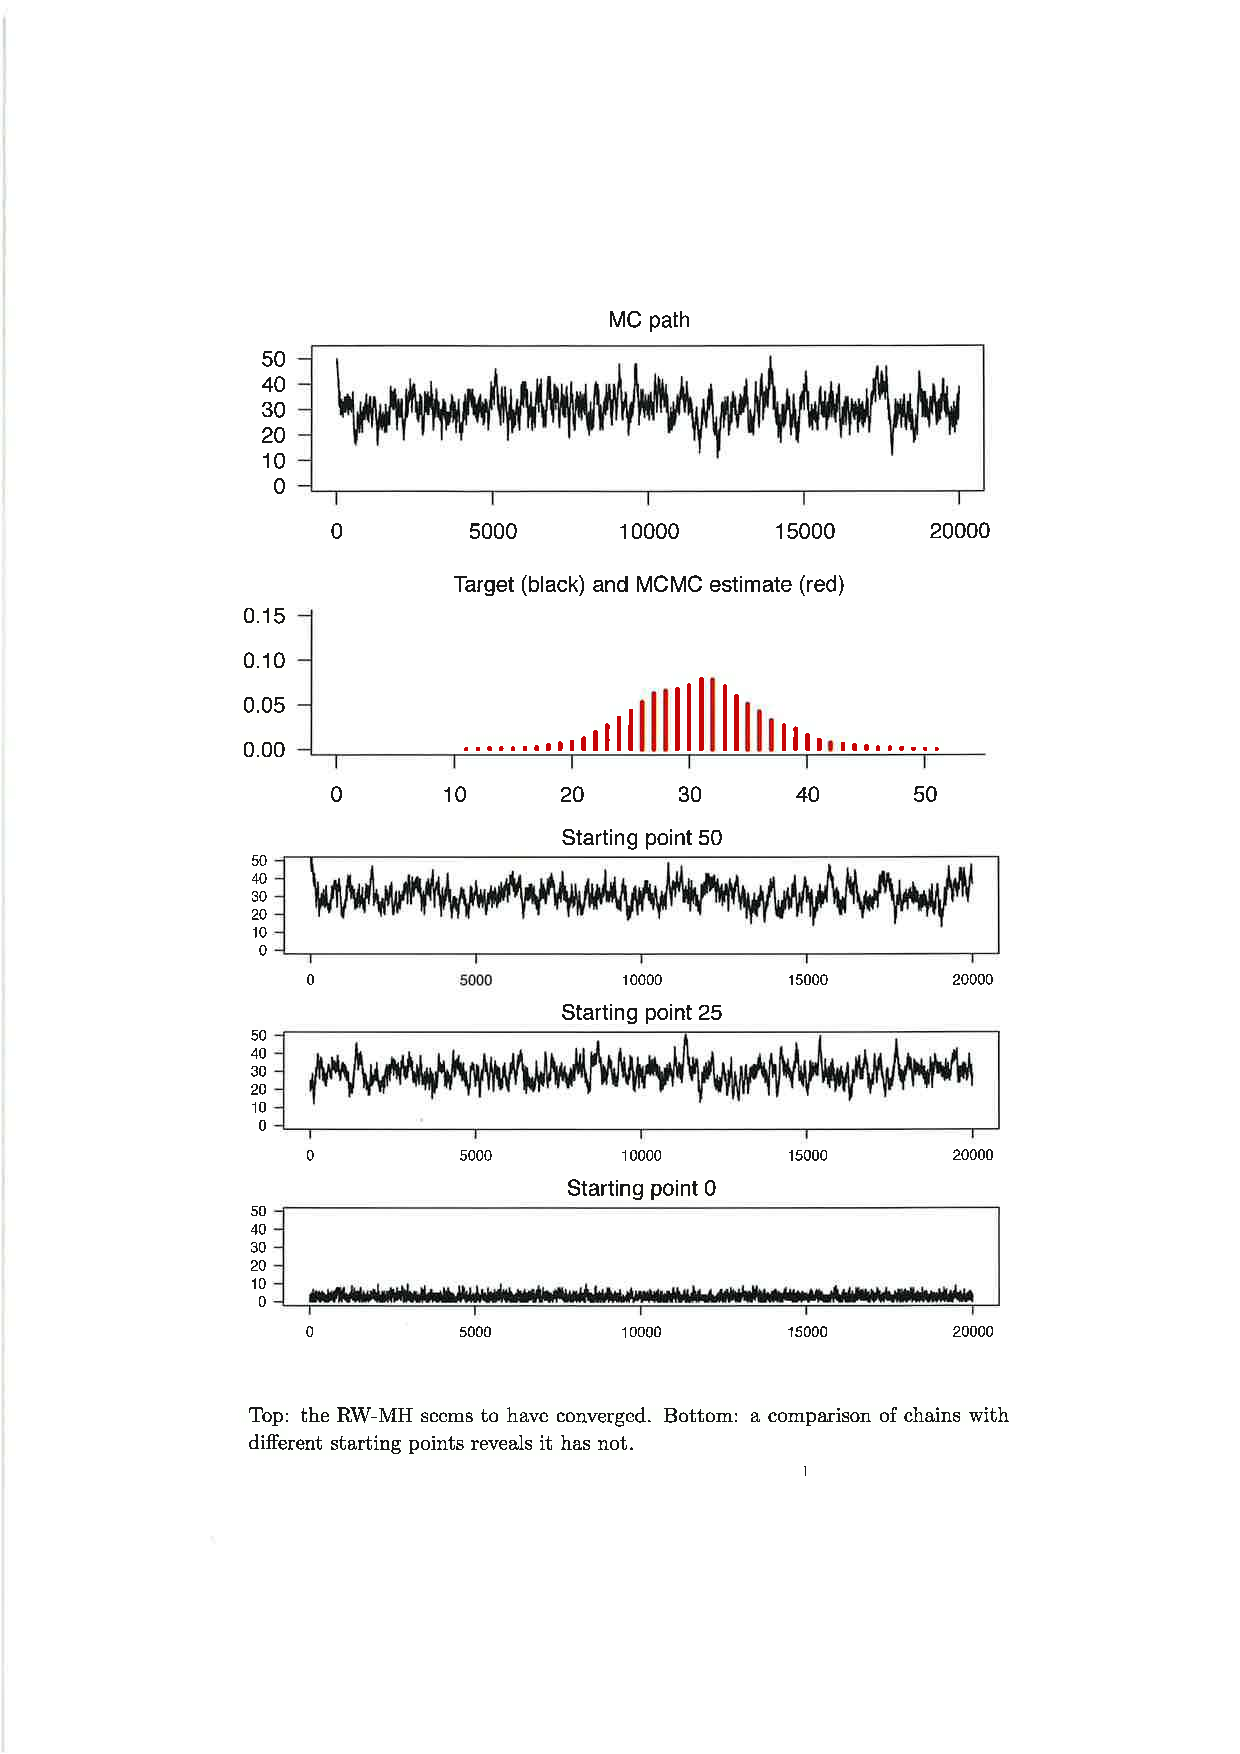
\includepdf[pages=-,pagecommand={}]{external/fake conv}
Extensions and other methods:
\begin{itemize}
    \item \textbf{Reversible jump MCMC}: it moves among spaces of different dimensions.  
    \item \textbf{Langevin algorithms} or \textbf{gradient-based MCMC}: is it inspired by the Langevin diffusion
    \begin{equation*}
        dX_t = \frac{1}{2} \frac{d}{dX_t} \log\pi(X_t)dt + dB_t
    \end{equation*}
    It uses information on the gradient of $\pi$ to move towards regions of higher density.
\end{itemize}
There is a principle (Goldilocks's principle of MCMC): the variance of the steps has to be not too large, not too small.
	\section{Continuous time Markov chains}
	\begin{definition}
		A \enf{continuous time Markov chain (CTMC)} is a stochastic process $\{X(t), t \in T\}$ with index set $T=[0,+ \infty)$ taking values in a countable set $S$, s.t. 
		\begin{equation*}
			\mathbb{P}(X(t_n)=i_n | X(t_0)=i_0, \dots, X(t_{n-1})= x(t_{n-1}))
		\end{equation*}
		i.e. the Markov property holds for all $i_0, \dots, i_n \in S$ and $0\leqslant t_0 < \dots < t_n$. \\
		We can define the transition probability 
		\begin{equation*}
			p_{ij}(s,s+t):= \mathbb{P}(X(s+t)=j|X(s)=i)
		\end{equation*}
		for $t>0$, which we assume are time homogeneoCus, i.e. depend on $t$ not on $s$. Hence we can define 
		\begin{equation*}
			p_{ij}(t):= p_{ij}(0,t)
		\end{equation*}
		since $p_{ij}(s,s+t)= p_{ij}(0,t)$.\\
		Set \[p_{ij}(0):=\delta_{ij}=\begin{cases}
			1 &i=j\\
			0 &i\neq j.
		\end{cases}\]
	\end{definition}
	\begin{example}
		The Poisson process with intensity $\lambda>0 $ is defined by $X(0)=0$ a.s. and 
		\begin{equation*}
			p_{ij}(t)= \frac{(\lambda t)^{j-1}e^{-\lambda t}}{(j-i)!}, \hspace{0.5 cm} j \geqslant 1
		\end{equation*}
		and $0$ elsewhere. We see it is time-homogeneous on $S = \mathbb{Z}_+$. The increments are s.t.
		\begin{equation*}
			X(s+t)-X(s) \sim Poisson (\lambda t)
		\end{equation*}
		and if we set $s=0$, then $X(t) \sim Poisson(\lambda t)$.
	\end{example}
	\begin{exercise}
		Show that the transition function of a MTMC, together with an initial distribution, determines all joint distribution 
		\begin{equation*}
			\mathbb{P}( X(t_0)=i_0, \dots, X(t_{n})= x(t_{n}))
		\end{equation*}
		for all choice of $i_0, \dots, i_n$ and $t_o <\dots < t_n$. \\
	\end{exercise}
	Denote $P_t$ the square matrix with entries $\{p_{ij}(t)\_{i, j \in S}$. \\
	the family of $\{P_t\}_{t\geqslant 0}$ is called \enf{transition semigroup}, since:
	\begin{itemize}
		\item $\sum_{j \in S} p_{ij} = 1$: row sum
		\item $P_0=I$ (i.e. $p_{ij}(0):=\delta_{ij}$)
		\item $P_{t+s}= P_t P_s$:  \enf{semigroup property}, namely the Chapman-Kolmogorov's equations 
		\begin{equation*}
			p_{ij}(s+t)= \sum_{k \in S} p_{ik}(s) p_{kj}(t)
		\end{equation*}
	\end{itemize}
	We will assume $P_t$ is continuous at the origin (called \textit{standard})
	\begin{equation*}
		p_{ij}(t) \rightarrow \delta_{ij} \hspace{0.5 cm} t \rightarrow 0
	\end{equation*}
	which implies continuity at all $t>0$.\\
	$P_t$ is parametrized by time, and ideally we would like on object similar to the transition matrix for DTMC's, , relative to the temporal unit. We look at infinitesimal intervals. 
	\begin{definition}
		The matrix $Q$ given by 
		\begin{equation*}
			Q= \frac{d}{dt}P_t |_{t=0}
		\end{equation*}
		is called infinitesimal generator of the chain, and its entries $(q_{ij})_{i,j \in S}$ are called \enf{infinitesimal rates}.
	\end{definition}
	\begin{proposition}
		Let $P_t$ be a continuous transition semigroup on $S$ countable. For all $i,j$ the quantity $q_{ij}:=p'_{ij}(0)$ exists and 
		\[q_{ij} \in
		\begin{cases}
			[0,\infty) & j \neq i \\
			[-\infty, 0] & j = i \\
		\end{cases}
		\]
		For $j \neq i$
		\begin{equation*}
			q_[ij] = \lim_{h \rightarrow 0} \frac{p_{ij}(h) - \overbrace{p_{ij}(0)}^{0}}{h}
		\end{equation*}
		%In a small time interval there is a  negligibile probability that the chain goes to (?infinity)
	\end{proposition}
	\begin{itemize}
		\item  $\implies p_{ij}(h)=q_{ij}h + o(h)$ 
		\item  $\implies X$ goes to $j$ from $i$ with probability approximately $q_{ij}h $.
		\item  $\implies o(h)$ collects the error of approximation and all other events (for example, $X$) goes to $k$ before $j$).
	\end{itemize}
	So the chain has at most one jump at each instant. When $j=i$, since $p_{ii}(0) = 1$, the above calculation gives $q_{ii} \leqslant 0$. \\
	Sometimes we will denote $q_i = - q_{ii}$.
	\begin{definition}
		A state $i$ is called
		\begin{itemize}
			\item \enf{absorbing} if $q_i = 0$
			\item \enf{stable} if $0 < q_i < \infty$
			\item \enf{instantaneous} if $q_i = \infty$ 
		\end{itemize}
		If $\sup_{i \in S} q_i < \infty, Q$ is \textbf{stable}. \\
		If $q_i = \sum_{j \neq i} q_{ij}, \hspace{0.2 cm} \forall i \in S, Q $ is called \enf{conservative}.     
	\end{definition}
	\begin{remark}
		The absolute value of the diagonal entry equals the sum of the off-diagonal entries.
	\end{remark}\begin{equation*}
		1 = \sum_{j \in S} p_{ij}(h) = \sum_{j \neq i} p_{ij}(h) + p_{ii}(h)
	\end{equation*}
	which leads to 
	\begin{equation*}
		\frac{1-p_{ii}(h)}{h} = \sum_{j \neq i} \frac{p_{ij}(h)}{h}
	\end{equation*}
	Taking the limit as $h$ decreases to $0$, we get
	\begin{equation*}
		q_i = \lim_{h \downarrow 0} \sum_{j \neq i} \frac{p_{ij}(h)}{h}
	\end{equation*}
	If limit and sum exchange, we get 
	\begin{equation*}
		q_i = \sum_{j \neq i} q_{ij} \implies \sum_{j \in S} q_{ij} = 0
	\end{equation*}
	\begin{remark}
		Conservativity comes from the fact that transition probabilities conserve the mass.
	\end{remark}
	We assumed we had the transition probabilities are available but this is rarely the case. In many cases, when we move on to general and complex spaces, probabilities are specified through the generator (instead of the transition semigroup).
	We are going to argument later that this gives complete information about the process too, but if we have the generator, how can we check that the implied process is well defined? We need criteria to be checked on the generator. Often, only $Q$ is available, while $P_t$ is unknown. So, this identity relates to the conservation of probability mass by the transition semigroup. So it is enough to check that $Q$ row sums are null (to verify this condition). \\
	If $Q$ is stable and conservative, $q_i$ is interpreted as the rate of leaving the state $i$. So
	\begin{equation*}
		p_{ii}(h) = 1-q_i h + o(h) 
	\end{equation*}
	If 
	\begin{itemize}
		\item $q_i = 0$, then $X$ leaves $i$ at rate $0$, so $i$ is absorbing. 
		\item $q_i = \infty$, then $x$ leaves the state $i$ instantaneously. 
	\end{itemize}
	\begin{proposition}
		A CTMC with finite state space is always stable and conservative.
	\end{proposition}
	So we can reverse the statement, saying that trouble scenario happen when the chain is not stable or not  conservative.
	\begin{example}
		Consider $X$ on $\mathbb{Z}_+$ with 
		\begin{equation*}
			q_{i,i+1}= \lambda \hspace{0.5 cm} q_{i,i-1}= i \hspace{0.5 cm} q_{ii}= -(\lambda + i)
		\end{equation*}
		and $0$ elsewhere. $Q$ is conservative ($P_t$ would be well defined, if we knew it) but 
		\begin{equation*}
			\sup_{i \in S} q_i = \sup_{i \geqslant 0} \lambda + i = \infty
		\end{equation*}
		so it is not stable. \\
		The meaning of this distinction will be treated later.
	\end{example}
	\begin{definition}
		A general class of stable and conservative CTMC's is given by \textbf{regular jump processes} such that 
		\begin{itemize}
			\item their paths are piecewise constant: for almost all $\omega$ and all $t \geqslant 0, \exists \varepsilon = \varepsilon(t,\omega)$ such that 
			\begin{equation*}
				X(t+s,\omega) = X(t,\omega) \hspace{0.5 cm} \forall s \in [0,\varepsilon]
			\end{equation*}
			This means that the chain remains where it is for a positive amount of time. 
			\item they have finitely many points of discontinuity in every bounded time interval.
		\end{itemize}
	\end{definition}
	The typical behaviour is the one represented in Figure \ref{regjump}. %metti figura. sì capo \\
	For example, \textbf{explosive chains} are not regular in the above sense (see Figure \ref{xplchain}): these chains have closer and closer jumps until there are infinitely many around $x=s$.%metti altra figura). fatto capo\\
	
	\begin{minipage}{0.5\textwidth}
		\begin{figure}[H]
			\centering
			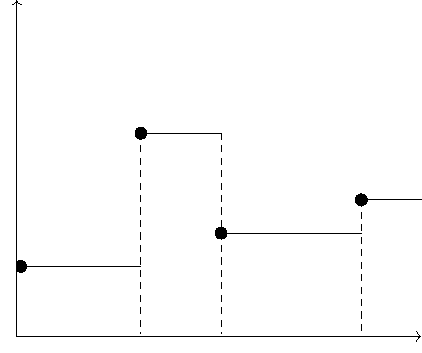
\includegraphics[scale=0.6]{standalones/pdfs/regjump}
			\caption{Regualar jumps process}
			\label{regjump}
		\end{figure}
	\end{minipage} \hfill
	\begin{minipage}{0.45\textwidth}
		\begin{figure}[H]
			\centering
			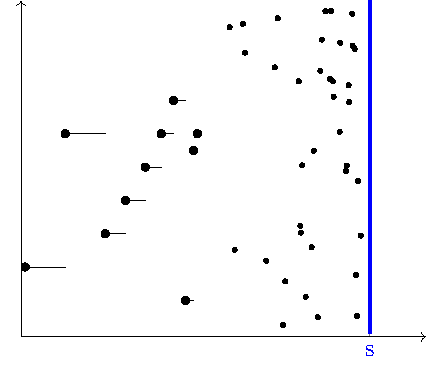
\includegraphics[scale=0.6]{standalones/pdfs/xplosive}
			\caption{explosive chain}
			\label{xplchain}
		\end{figure}
	\end{minipage}
	
	\begin{example}
		\enf{Poisson process}
		\begin{align*}
			&p_{ij}(t)=\frac{(\lambda t)^{j-i}e^{-\lambda t}}{(j-i)!}\qquad j\geqslant 1\\
			\implies &p_{ii}(t)=e^{-\lambda t}\\
			&p_{i,i+1}(t)=\lambda t e^{-\lambda t}\\
			&p_{i,i+k}(t)=\frac{(\lambda t)^{k}e^{-\lambda t}}{k!}\\
			\implies &q_{ii}=-\lambda,\quad q_{i,i+1}=\lambda,\qquad\text{and 0 elsewhere.}
		\end{align*}
		\textit{Interarrival times}: $T_i$ waiting time in $i$.
		\begin{align*}
			\mathbb{P}(T_0 > t) &= \mathbb{P}(X(t) = 0|X(0) = 0) = e^{- \lambda t}\\
			\implies \mathbb{P}(T_0 < t) &= 1-e^{-\lambda t} \implies T_0 \sim \text{Exp}(\lambda)
		\end{align*}
		So $\prob(T_i>t|T_0=t_0,\ldots,T_{i-1}=t_{i-1})=$
		\begin{align*}
			s &= t_0+\ldots+t_{i-1}\\
			&=\prob(x(s+t)=i|x(s)=i)=e^{-\lambda t}\\
			&\implies T_i\sim\text{Exp}(\lambda)
		\end{align*}
	\end{example}
	\begin{example}(Birth and Death processes)\\
		Denote B\&D$(\lambda _i, \mu_i)$ such that 
		\[q_{ij} = 
		\begin{cases}
			\lambda_i & j = i+1  \hspace{0.5 cm} i \geqslant 0 \\
			\mu_i  & j = i-1  \hspace{0.5 cm} i > 0 \\
			0 & \text{elsewhere} \\
		\end{cases}
		\]
		\begin{equation*}
			q_{ii} = - (\lambda _ i + \mu_i)
		\end{equation*}
		%figura arriva!!
		\begin{figure}[H]
			\centering
			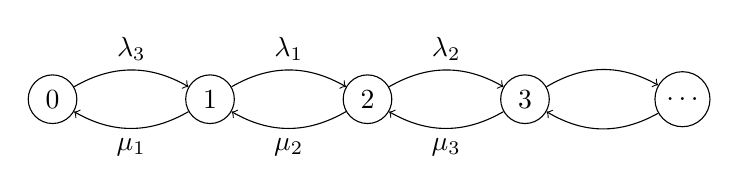
\begin{tikzpicture}[->,node distance=2cm]
				\node[circle,draw](zero){0};
				\node [circle,draw] (one) [right of=zero] {1};
				\node [circle,draw] (two) [right of=one] {2};
				\node [circle,draw] (three) [right of=two] {3};    
				\node [circle,draw] (dots) [right of=three]{$\ldots$};
				\path (one) edge [bend left] node [above] {$\lambda_1$} (two);
				\path (two) edge [bend left] node [above] {$\lambda_2$} (three);
				\path (three) edge [bend left] node [below] {$\mu_3$} (two);
				\path (two) edge [bend left] node [below] {$\mu_2$} (one);
				\path (three) edge [bend left] node [below] {} (dots);
				\path (dots) edge [bend left] node [below] {} (three);
				\path (zero) edge [bend left] node [above] {$\lambda_3$} (one);
				\path (one) edge [bend left] node [below] {$\mu_1$} (zero);
			\end{tikzpicture}
			\label{bedcontinuous}
		\end{figure} whose invariant $\pi$ is the uniform on on $S_0$. Let $\tau$ be a finite random time on $\N$, independent of $Y$, such that:  
	\end{example}
	Special cases:
	\begin{itemize}
		\item $\mu_i=0 \;\forall i, \lambda_i > 0$ \textbf{Birth process} which can be 
		\begin{itemize}
			\item [$\star$] Poisson
			\item [$\star$] $\lambda_i = \underbrace{\lambda}_{\mathclap{\text{per capita birth rate}}}\cdot i $ (\enf{Yule process})
		\end{itemize}
		$\lambda_i = \lambda \cdot i + c$, adding immigration rate $c$.
		\item $\lambda_i = 0 \forall i, \mu_i > 0$ (\enf{Pure death process})
	\end{itemize}
	For example, if 
	\begin{equation*}
		\lambda_i = \lambda \cdot i, \hspace{0.5 cm} \mu_i = \mu \cdot i
	\end{equation*}
	the transition probabilities are very complicated to find, like in the following case: the process has $i = 1$
	\begin{equation*}
		p_{1j}(t) = (1-\mu \gamma) (1-\lambda \gamma) (\lambda \gamma)^{j-i}
	\end{equation*}
	where 
	\begin{equation*}
		\gamma= \frac{e^{(\lambda-\mu) t} - 1}{\lambda e^{(\lambda - \mu)t}-\mu}
	\end{equation*}
	If $X$ is specified only through the generator $Q$, a general task is to be able to describe the transition semigroup (which is difficult in general). \\
	A first tool to do so is given by the so called \textbf{Kolmogorov's equations}.
	\begin{theorem}
		Let $Q$ be stable and conservative. Then, $P_t$ and $Q$ satisfy:
		\begin{itemize}
			\item The \enf{backward equation}
			\begin{equation*}
				P'_t =  Q P_t \hspace{1 cm} p'_{ij}(t) = \sum_{k \in S} q_{ik}p_{kj}(t)
			\end{equation*}
			\item If 
			\begin{equation*}
				\sum_{k \in S} p_{ik}(t) q_k < \infty
			\end{equation*}
			the \enf{forward equation}
			\begin{equation*}
				P'_t = P_t Q \hspace{1 cm} p'_{ij}(t) = \sum_{k \in S} p_{ik}(t)q_{kj}
			\end{equation*}
		\end{itemize}
	\end{theorem}
	\begin{exercise}
		Prove the forward equation for $S$ finite using CK and linearization.\\
		The intuition consists in thinking about the backwards equation.
		\begin{figure}[H]
			\centering
			    \begin{tikzpicture}[-,>=stealth', line width=0.5pt, node distance=0.5cm]

        \node [circle, draw,  fill, label=left:$i$] (two) []{};

        \node [circle, draw,  fill] (c) [right=1cm of two]{};
        \node [circle, draw,  fill] (b) [above of=c] {};
        \node [circle, draw,  fill] (a) [above of= b]{};
        
        
        \node [circle, draw,  fill] (d) [below of=c]{};
        \node [circle, draw,  fill] (e) [below of=d]{};
        

        \node [circle, draw, fill, label=right:$j$,  circle] (j) [right= 1 cm of c]{};

        \path (two) edge node [below] {} (a);
        \path (two) edge node [below] {} (b);
        \path (two) edge node [below] {} (c);
        \path (two) edge node [below] {} (d);
        \path (two) edge node [below] {} (e);

        \path (a) edge node [below] {} (j);
        \path (b) edge node [below] {} (j);
        \path (c) edge node [below] {} (j);
        \path (d) edge node [below] {} (j);
        \path (e) edge node [below] {} (j);

        \node[circle][above right=12pt and 6pt of two]{$h$};
         \node[circle][above left=12pt and 6pt of j]{$t$};
    \end{tikzpicture}
		\end{figure}
		To obtain an intuition for the forward equation, let the second interval go to $0$.\\
		\\
		In principle (which boils down to simple cases), one could solve the Kolmogorov's equations to find the semigroup. \\
	\end{exercise}
	\begin{exercise}
		Consider the generator of the Poisson process:
		\begin{equation*}
			q_{i,i+1}=\lambda \hspace{1 cm} q_{ii} = - \lambda
		\end{equation*}
		Derive the transition probabilities from Kolmogorov's equations.  
	\end{exercise}
	First of all, we are going to analyze an example to show how Kolmogorov equations can be used and also their complexity. Let's recall the Kolmogorov Backward Equation
	\begin{equation*}
		p'_{ij}(t) = \sum_{k \in S} q_{ik}p_{kj}(t)
	\end{equation*}
	and the Kolmogorov Forward Equation
	\begin{equation*}
		p'_{ij}(t) = \sum_{k \in S} p_{ik}(t) q_{kj}
	\end{equation*}
	which provide a relationship between $P_t$ and $Q$. In simple cases they can be solved. 
	\begin{example}\enf{Poisson Process}
		\begin{equation*}
			q_{i,i+1} = \lambda \hspace{1 cm} q_{ii} = -\lambda \text{ and } 0 \text{ elsewhere}
		\end{equation*}
		Let's consider the K.F.E. and let's consider 
		\begin{itemize}
			\item $j=i$:
			\begin{equation*}
				p'_{ii}(t) = p_{ii}(t) q_{ii} = -\lambda p_{ii}(t)
			\end{equation*}
			$k = i$ necessarily. This yields
			\[
			\begin{cases}
				p_{ii}(t) & = c e ^{-\lambda t} \\
				p_{ii}(0) & = 1 \implies c = 1 \\ 
			\end{cases}
			\]
			We find the constant using the boundary condition $p_{ii}(0) = 1 $.
			\item $j > i$
			\begin{figure}[H]
				\centering
				\documentclass{standalone}			
\usepackage{../pacco}	
\begin{document}
\begin{tikzpicture}[-,>=stealth', line width=0.5pt, node distance=0.5cm]
	
	\node [circle, draw,  label=left:$i$] (two) []{};
	\node [circle, draw] (tre) [above of=two] {};
	\node [circle, draw] (quattro) [above of=tre] {};
	\node [circle, draw] (cinque) [above of=quattro] {};
	
	\node [circle, draw] (c) [right=3cm of two]{};
	\node [circle, draw] (b) [above of=c] {};
	\node [circle, draw] (a) [above of= b]{};
	
	
	\node [circle, draw] (d) [above of=a]{};
	\node [circle] (e) [above of=d]{$t^-$};
	
	
	\node [circle, draw, label=right:$j$,  circle] (j) [right= 1 cm of d]{};
	\node [circle,draw](ciao)[below of=j]{};
	\node [circle,draw](come)[below of=ciao]{};
	\node [circle,draw](stai)[below of=come]{};
	\node [circle](MALE)[above of=j]{$t$};
	
	\path (two) edge [->]node [below] {} (a);
	\path (two) edge [->]node [below] {} (d);
	\path (a) edge [->]node [below] {} (j);
	\path (d) edge [->]node [below] {} (j);
\end{tikzpicture}
\end{document}

			\end{figure}
				\begin{align*}
				p'_{ij}(t) &= p_{i,j-1}(t) q_{j-1,j} + p_{ij}(t) q_{jj}\\
				&= \lambda p_{i,j-1}(t) - \lambda p_{ij}(t)
			\end{align*}
			Now, multiply by $e^{\lambda t}$ and get from
			\begin{equation*}
				p'_{ij}(t) = \lambda p_{i,j-1}(t) - \lambda p_{ij}(t) 
			\end{equation*}
			the following
			\begin{equation*}
				\underbracket{e^{\lambda t} p'_{ij}(t) + \lambda e^{\lambda t}}_{\frac{\dif}{\dif t}\left\{e^{\lambda t}p_{ij}(t)\right\}}=\lambda e^{\lambda t}p_{i,j-1}(t)
			\end{equation*}
			%manca un pezzo
			
			assume $p_{i,j-1}(t) = \frac{(\lambda t)^{j-i-1}e^{-\lambda t}}{(j-i-1)!}$
			and integrate to get
			\begin{equation*}
				\frac{d}{dt}(e^{\lambda t} p_{ij}(t)) = \lambda \cancel{e^{\lambda t}} \frac{(\lambda t)^{j-i-1}\cancel{e^{-\lambda t}}}{(j-i-1)!} = \frac{\lambda^{j-i}}{(j-i-1)!} t ^{j-i-1}
			\end{equation*}
			Which leads to 
			\begin{equation*}
				e^{\lambda t}p _{ij}(t) =  \frac{\lambda^{j-i}}{(j-i-1)!} \frac{t ^{j-i-1} }{j-i} + c'
			\end{equation*}      
			which yields
			\[
			\begin{cases}
				p_{ij}(t) &= \frac{(\lambda t)^{j-i}e^{-\lambda t}}{(j-i)! } + c' \\
				p_{ij}(0) = 0 \implies c' = 0
			\end{cases}
			\]
			\end{itemize}
	\end{example}
What are the general solutions of the Kolmogorov equations?
\begin{theorem}
	Let $S$ be finite. Then
	\begin{equation*}
		P_t = e^{tQ}, \hspace{1 cm} P_0 = I
	\end{equation*}
	is a stochastic semigroup and the unique solution of the K.E.'s. 
\end{theorem}
\begin{remark}
		The matrix exponential
	\begin{equation*}
		e^{tQ}:= \sum_{n \geqslant 0} \frac{(tQ)^n}{n!} 
	\end{equation*}
	is convergent component-wise since $e^{t q_{ij}} < \infty, \forall t > 0$. 
\end{remark}
If $A,B$ commute, 
\begin{equation*}
	e^{A+B} = e^A e ^B
\end{equation*}
which yields
\begin{equation*}
	P_{t+s} = e^{t+s}Q = e^{tQ} e^{sQ} = P_t P_s
\end{equation*}
Intuition: consider 
\begin{equation*}
	\begin{split}
		p_{ij}(t)&= \delta_{ij}+q_{ij}t+ o(t) \hspace{0.5cm}\forall i,j\\
		P_t&=I+tQ+ o(t)
	\end{split}
\end{equation*}
Use the semigroup property to split $[0,t]$ into $n$ subintervals, so 
\begin{equation*}
	P_t= \underbrace{P_{\frac{t}{n}} \dots P_{\frac{t}{n}}}_{n \text{ times }} = (I+tQ+ o(t))^n
\end{equation*}
which generate the exponential $e^{tQ}$ as $n \rightarrow + \infty$. The generator also gives important information about the trajectories of the chain. \\
\begin{definition}
		Define the Holding Times (or waiting).
	\begin{equation*}
		T_i = \inf\{t \geqslant 0: X(s+t)\neq i | X(s)=i\}
	\end{equation*}
	in state $i\in S$, with $T_i=\infty$ if $i$ absorbing.
\end{definition}
\begin{proposition}
		Let $X$ be a regular jump CTCM with generator $Q$, and let $T_i$ be the first holding time given $X(0)=i$. Then\begin{itemize}
		\item $T_i \sim Exp(q_i)$
		\item for $j \neq i$
		\begin{equation*}
			\mathbb{P}(X(T_i)=j|X(0)=i) = \frac{q_{ij}}{q_i}
		\end{equation*}
		and these are independent. 
	\end{itemize}
\end{proposition}
Interpretation:
\begin{figure}[H]
	\centering
	\begin{tikzpicture}%[scale=0.8]
\begin{axis}[
                xlabel=\empty,
                x axis line style={->,opacity=100},
                ylabel=\empty,
                xmin=-1, xmax=100,
                ymin=-1, ymax=100,
                axis y line=left,
                y axis line style={->,opacity=100},
                ytick={20,60,40},
                yticklabels={$h$,$j$,$i$},
                xtick=\empty,
                axis x line*=bottom
                        ]
                        \draw [dashed, thick] (0,20)--(95,20) node[RedViolet,circle,midway,inner sep=2pt,yshift=10pt]{Exp($q_{ih}$)};
                        \draw [dashed, thick](0,60)--(95,60) node[RedViolet,circle,midway,inner sep=2pt,yshift=10pt]{Exp($q_{ij}$)};
                        \draw [dashed, thick](0,40)--(95,40);

\end{axis}
\end{tikzpicture}
\end{figure}
We can immagine that at every state there is a poisson process that rings at every time, exponential (?????).\\
There is a Poisson prosses with rate $q_{ij}$ each $j \neq i$ acting as a clock (all independent). Competing clocks: the first ringing sets the new state.\clock[0.1]{10}{3}{6} \\
We know 
\begin{equation*}
	\begin{split}
		Z_k &\stackrel{ind}{\sim} Exp (\lambda_k)\\
		&\implies  \min_k Z_k \sim Exp (\sum_k \lambda_k) \hspace{0.5 cm} \text{ shortest interval}\\
		&\mathbb{P}(\min_{k\neq i} Z_k=Z_j)= \frac{\lambda_j}{\sum_h \lambda_h} hspace{0.5 cm} \text{ prop of j-th is the fist to ring}
	\end{split}
\end{equation*}
So $T_i \sim Exp(\sum_{j\neq i}q_{ij})= Exp(q_i)$ and given $T_i$, the probability of going to $j$ is 
\begin{equation*}
	\frac{q_{ij}}{\sum_{j\neq i}q_{ij}}= \frac{q_{ij}}{q_i}
\end{equation*}
We can extend the above to the entire trajectory of the CTMC through the strong Markov property:
\begin{theorem}
	A regular jump CTMC $X$ with generator $Q$ is a strong markov process, i.e. 
	if $\tau$ is a stopping time w.r.t. to $\mathcal{F}_t ^X= \sigma(X_u, u \leqslant t)$, 
	conditional on $\tau <\infty$ and $X(\tau)=i$, $\{X(\tau+t), t\geqslant 0\}$ is a CTMC with initial distribution $\delta_i$ and generato $Q$, independent of $\{X(u), u\leqslant t\}$
\end{theorem}
If we now denote 
\begin{itemize}
	\item $T^{(1)}, T^{(2)}, \dots$ successive holding times 
	\item  $S_n= \sum_{i=1}^n T^{(i)}$ jumps times (Stopping times)
	\item $X_n:= X(S_n)$
\end{itemize}
\begin{figure}[H]
	\centering
	\begin{tikzpicture}%[scale=0.8]
\begin{axis}[
                xlabel=\empty,
                x axis line style={->,opacity=100},
                ylabel=\empty,
                xmin=-1, xmax=100,
                ymin=-1, ymax=100,
                axis y line=left,
                y axis line style={->,opacity=100},
                ytick={20,60,40},
                yticklabels={$X_0$,$X(S_1)=X_1$,$X(S_2)=X_2$},
                xtick={30,60},
                xticklabels={$S_1$,$S_2$},
                axis x line*=bottom
                        ]
                        \draw (0,20)--(30,20) node[circle,fill=RedViolet, pos=0,inner sep=2pt]{};
                        \draw (30,60)--(60,60) node[circle,fill=RedViolet, pos=0,inner sep=2pt]{};
                        \draw (60,40)--(95,40) node[circle,fill=RedViolet, pos=0,inner sep=2pt]{};
                        \draw[dashed] (30,20)--(30,0);
                        \draw[dashed] (60,60)--(60,0);
                        \draw[dotted,thin] (0,40)--(60,40);
                        \draw[dotted,thin] (0,60)--(30,60);
\end{axis}
\node[RedViolet,below right=0.1cm and 0.43cm, font=\footnotesize] (T) {Exp$(q_{x_0})$};
\node[RedViolet,below right=0.1cm and 2.55cm, font=\footnotesize] (Te) {Exp$(q_{x_1})$};
\node[above right=0.0cm and 0.63cm, font=\footnotesize] (T) {$T^{(1)}$};
\node[above right=0.0cm and 2.75cm, font=\footnotesize] (Te) {$T^{(2)}$};
\end{tikzpicture} 
\end{figure}
$X_n$ is  a DTMC called \textbf{embedded chain} with transition probabilities 
\begin{equation*}
	p_{ij}= \begin{cases}
		\frac{q_{ij}}{q_i} \hspace{0.5cm}&j \neq i \\
		0 &j =i
	\end{cases}
\end{equation*}
Note $X_n$ is not allowed self transitions. Given $(X_n)_{n \geqslant 1}$
\begin{equation*}
	T^{(n)}\stackrel{\text{ind}}{\sim} Exp(q_{X_{n-1}})
\end{equation*}
We have factorised the state set of the chain.
\begin{example}
	\enf{Birth and Death $(\lambda _i, \mu_i)$}:
	\[q_{ij} = 
	\begin{cases}
		\lambda_i & j = i+1, i \geqslant 0 \\
		\mu_i & j= i-1, i > 0\\
		0 &\text{ elsewhere}
	\end{cases}
	\]
	\begin{equation}
		q_{ii} = - (\lambda _i + \mu_i), \hspace {0.5 cm} q_i = \lambda _ i + \mu_i
	\end{equation}
	$\implies$ holding times in $i$ are 
	\begin{equation*}
		T_i \sim \text{ Exp} (q_i) = \text{ Exp }(\lambda_i + \mu_i)
	\end{equation*}
	$\implies$ embedded chain $X_n$ has transitions 
	\[p_{ij}
	\begin{cases}
		\frac{\lambda_i}{ \lambda _ i + \mu_i} & j = i+1 \\
		\frac{\mu_i}{ \lambda _ i + \mu_i} & j = i-1 \\
		0 & \text{ elsewhere}
	\end{cases}
	\]
\end{example}
A corollary of the above argument is the following:
\begin{proposition}
	Two regular jump CTMC's woth the same $Q$, and initial distributions, have the same transition semigroup.
\end{proposition}
This is important since we know we can proceed even without the semigroup. Embedded chain and holding times are fully determined by th egenerator $Q$, which therefore provides an equivalent characterization of the CTMC. The above suggests an imemdiate strategy to simulate the chain's trajectory:
\begin{itemize}
	\item Draw $X_0$ from the initial distribution
	\item for $n \geqslant 1, $if $X_{n-1} = i$
	\begin{itemize}
		\item [-] draw $T \sim \text{Exp}(q_i)$
		\item [-] given $T = t$, set
		\begin{equation*}
			X(t) = j \text{ with probability } \frac{q_{ij}}{q_i}
		\end{equation*}
		called \textbf{gillespie} algorithm.
	\end{itemize}
\end{itemize}
So, given a CTMC and generator - for every state - we draw the exponential with parameter represented by the first state and then we draw the normalized probabilities, iterating this process.\\
Another subclass of CTMC which allows for an explicit description of $P_t$ is the one defined below.
\begin{definition}
	Let $Y_n$ be a CTMC with transition matrix $\hat{P}$, and $N(t)$ a Poisson process with rate $\lambda$, independent of $Y_n$. The process
	\begin{equation*}
		X(t) := Y_{N(t)}   
	\end{equation*}
	is called \textbf{uniform chain with jump matrix} $\hat{P}$.         
\end{definition}
\begin{figure}[H]
	\centering
	\begin{tikzpicture}%[scale=0.8]
\begin{axis}[
                xlabel=\empty,
                x axis line style={->,opacity=100},
                ylabel=\empty,
                xmin=-1, xmax=100,
                ymin=-1, ymax=100,
                axis y line=left,
                y axis line style={->,opacity=100},
                ytick={20,60,40},
                yticklabels={$Y_0$,$Y_1$,$Y_2=Y_3$},
                xtick=\empty,
                axis x line*=bottom
                        ]
                        \draw (0,20)--(30,20) node[circle,fill=RedViolet, pos=0,inner sep=2pt]{};
                        \draw (30,60)--(50,60) node[circle,fill=RedViolet, pos=0,inner sep=2pt]{};
                        \draw (50,40)--(85,40) node[circle,fill=RedViolet, pos=0,inner sep=2pt]{};
                        \draw (85,40)--(100,40) node[circle,fill=RedViolet, pos=0,inner sep=2pt,label={self-transition}]{};
                        \draw[dashed] (30,20)--(30,0);
                        \draw[dashed] (50,60)--(50,0);
                        \draw[dashed] (85,40)--(85,0);
                        \draw[dotted,thin] (0,40)--(50,40);
                        \draw[dotted,thin] (0,60)--(30,60);
\end{axis}
\node[RedViolet,below right=0.1cm and 0.43cm, font=\footnotesize] (T) {Exp$(\lambda)$};
\node[RedViolet,below right=0.1cm and 2.15cm, font=\footnotesize] (Te) {Exp$(\lambda)$};
\node[RedViolet,below right=0.25cm and 4.3cm, font=\footnotesize\bf] (Te) {$\ldots$};
\end{tikzpicture} 
\end{figure}
We have 
\begin{equation*}
	X(t) = Y_n \hspace{0.5 cm} \forall t \text{such that } N(t) = n 
\end{equation*}
Such $N(t)$ is called \enf{subordinator} and $Y_{N(t)}$ is called \enf{subordiated} chain.
\begin{center}
	\begin{tabular}{m{2cm}|m{3.5cm}|m{3cm}}
		& \textbf{Holding times} & \textbf{Self transitions}  \\ \hline
		\textbf{Embedded chains} & $T^{(n)}\stackrel{\text{ind}}{\sim}\text{Exp}({q_{x-1}})$ & not allowed by construction\\ \hline
		\textbf{Uniform chains}&$T^{(n)}\stackrel{\text{\textcolor{Dandelion!50!black}{i.i.d.}}}{\sim}\text{Exp}(\lambda)$ & if $\hat{p}_{ii}>0$
	\end{tabular}
\end{center}
Why are they interesting? Uniform chains allow an explicit form for the semigroup. 
	\begin{proposition}
		Let $X$ be a uniform chain with jump matrix $\hat{P}$ and rate $\lambda$ Poisson subordinator. Then, the generator is written as
		\begin{equation*}
			Q = \lambda (\hat{P}-I), \hspace{0.5 cm} P_t = \sum_{n \geqslant 0} \frac{(\lambda t)^{n}e^{-\lambda t}}{n!} \hat{P}^n
		\end{equation*}
	\end{proposition}
\begin{proof2}
	$P_t$: write $p_{ij}(t)$ and condition on $N(t) = n$
	$Q$: differentiate $P_t$. 
\end{proof2}
The above representation for $P_t$ is consistent with $e^{tQ}$ (having $S$ finite):
\begin{align*}
	AB=BA\implies e^{A+B}&=e^Ae^B \\
	\implies e^{tQ}&=e^{\lambda t(\hat{P}-I)} \\
	&=e^{\lambda t \hat{P}}\underbracket{e^{\lambda t I}}_{\mathclap{e^{\lambda t}I\text{ since }I^n=I}}
\end{align*}
so
\[
e^{tQ}=e^{-\lambda t}\sum_{n\geqslant 0}\frac{(\lambda t)^n}{n!}\hat{P}^n=\sum_{n\geqslant 0}(\lambda t)^n\frac{e^{\lambda t}}{n!}\hat{P}^n.
\]
A regular jump CTMC $X(t)$ can be represented fully by means of:
\begin{itemize}
	\item an embedded chain $X_n := X(S_n)$
	\begin{equation*}
		S_n = \sum_{i = 1}^n T^{(i)}
	\end{equation*}
	sequence of visited states
	\item given $(X_n)_{n \geq 1}$
	\begin{equation*}
		T^{(i)} \stackrel{\text{ i.i.d.}}\sim \text{ Exp}(q_{X_{i-1}})
	\end{equation*}
	independently of $T^{(i-1)}$
\end{itemize}
We are going to introduce the \textbf{uniform chains} 
\begin{equation*}
	X(t) = Y_{N(t)}
\end{equation*}
where
\begin{itemize}
	\item $Y_n$ is a CTMC with transition matrix $\hat{P}$ such that $\hat{p}_{ii} \geq 0$
	\item $N(t) \sim$ Poisson$(\lambda t)$
\end{itemize}
$\implies Q = \lambda (\hat{P} - I)$.
Now, the question is: \textit{Can we reparameterize a generic CTMC which we assume to be regular }\textit{jump with generator $Q$ as a uniform chain (for which we can describe the semigroup)?} Hint:\\
$Q = \lambda (\hat{P} - I)$ generator of uniform chain.
We manupulate it as follows:
\begin{equation*}
	\lambda^{-1} Q = \hat{P} - I \implies \hat{P} = I + \lambda^{-1} Q 
\end{equation*} 
\textit{Can we identify this matrix $\hat{P}$ given $Q$?}\\

The answer is affirmative, under the specific constraint:
\begin{equation*}
	\sup_i q_i < \infty
\end{equation*}
If this condition holds (so we have a stable $Q$), take:
\begin{itemize}
	\item any number 
	\begin{equation*}
		\nu \geq \sup_i q_i = \sup_i \sum_{j \neq i} q_{ij}
	\end{equation*}
	if the chain is conservative
	\item holding times 
	\begin{equation*}
		T^{(n)} \stackrel{\text{i.i.d.}}\sim \text{Exp}(\nu)
	\end{equation*}
	(they are picked from the universal clock \clock[0.1]{6}{3}{11})
	\item jump probabilities 
	\begin{equation*}
		\hat{p}_{ij} = \frac{q_{ij}}{\nu}
	\end{equation*}
	that could leave us some mass when the state is left.

	\begin{align*}
	\hat{p}_{ii} &= 1- \sum_{j \neq i} \hat{p}_{ij} = 1-\sum_{j \neq i} \frac{q_{ij}}{\nu} \\
	&= 1-\frac{q_i}{\nu} = 1 + \frac{q_{ii}}{\nu} 
\end{align*}
$\implies \forall i,j$
\begin{equation*}
	\hat{p}_{ii}  = \delta_{ij} +  \frac{q_{ij}}{\nu}
\end{equation*}
which is equivalent, in matrix form, to saying
\begin{equation*}
	\hat{P}= I + \nu^{-1} Q
\end{equation*}
as hinted above.
\end{itemize}
(We picked $\nu$, which is a rate faster than all the other rates of the universal clock.\clock[0.1]{6}{3}{11})
$\implies$
\begin{equation*}
	P_t = \sum_{n \geq 0} \frac{(\nu t)^n e^{-\nu t}}{n!} \hat{P}^n
\end{equation*}
is the semigroup. Let's now analyze some examples:
\begin{example}
	We consider a two state chain, represented in the following Figure. The generator is Q = 
	$\begin{bmatrix}
		-\lambda & \lambda \\
		\mu & - \mu \\
	\end{bmatrix}$
	\begin{align*}
		T^{(n)}_0 &\stackrel{\text{i.i.d.}}\sim\text{Exp}(q_0) = \text{Exp} (\lambda) \text{  in state $0$} \\
		T^{(n)}_1 &\stackrel{\text{i.i.d.}}\sim\text{Exp}(q_1) = \text{Exp} (\mu) \text{  in state $1$)}
	\end{align*}
	\begin{itemize}
		\item embedded chain has transition
		$\begin{bmatrix}
			0 & 1 \\
			1 & 0 \\
		\end{bmatrix}$
	\end{itemize}
	Let's make it uniform:
	\begin{itemize}
		\item $\nu = \lambda + \mu$
		$\implies $
		\begin{equation*}
			\hat{T}^{(n)}_i \stackrel{\text{i.i.d.}}{\sim} \text{Exp}(\nu) = \text{Exp}(\lambda +\mu), \hspace{0.5 cm} i = q_1
		\end{equation*}
		\item jump matrix
		\begin{equation*}
			\hat{P}= I + \nu^{-1} Q
		\end{equation*}
		\begin{align*}
			\hat{p}_{01} = \frac{q_{01}}{\nu} = \frac{\lambda}{\lambda + \mu} & \hspace{1 cm} \hat{p}_{00} = 1 - \frac{\lambda}{\lambda + \mu} = \frac{\mu}{\lambda + \mu} \\
			\hat{p}_{10} = \frac{q_{10}}{\nu} = \frac{\mu}{\lambda + \mu} & \hspace{1 cm} \hat{p}_{11} =\frac{\lambda}{\lambda + \mu}  
		\end{align*}
	\end{itemize}
	So now, since 
	\begin{equation*}
		\hat{P}^{n} = \hat{P}  \text{    (check)}
	\end{equation*}
	and the chain is uniform:
	\begin{align*}
		p_{00}(t) &= \sum_{n \geq 0} \frac{(\nu t) ^n e^{-\nu t}}{n!} \hat{p}_{00}^{(n)}\\
		&= e^{-\nu t} + \sum_{n \geq 1} \frac{(\nu t) ^n e^{-\nu t}}{n!} \hat{p}_{00} \\
		&= e^{-\nu t} + \hat{p}_{00}(1-e^{-\nu t})\\
		&= \hat{p}_{00} + e^{-\nu t}(1-\hat{p}_{00}) \\
		&= \frac{\mu}{\lambda + \mu} + e^{-(\lambda + \mu) t} \frac{\lambda}{\lambda + \mu}
	\end{align*} 
\end{example}
\section{Stationarity}
Irreducibility and recurrence are inherited from the embedded chain. 
\begin{definition}
	$\pi$ (row vector) is an \textbf{invariant measure} for $X$ if 
	\begin{equation*}
		\pi P_t = \pi \quad \forall t \geq 0.
	\end{equation*}
	This is called \enf{global balance condition}.
\end{definition}

\begin{equation*}
	\sum_{i \in S} \pi_i p_{ij}(t) = \pi_j \quad \forall i, j
\end{equation*}
If $P_t$ is unknown, the above condition is impossible to be checked. Hence, we need a new criterion for $Q$. 
\begin{proposition}
		Let $X$ be irreducible and recurrent. Then, there exists an invariant measure $\pi$, which is unique up to a multiplicative constant. Furthermore, we have that 
	\begin{equation*}
		\pi P_t = \pi \quad \forall t \geq  0 \iff \pi Q = \underline{0}
	\end{equation*}
	where $\underline{0} = (0, \ldots,0)$
\end{proposition}
\begin{proof2}
		$S$ finite:
	\begin{align*}
		\frac{d}{dt} (\pi  P_t)_j &= \frac{d}{dt} \sum_i \pi_i p_{ij}(t) \\
		&= \sum_i \pi_i p'_{ij}(t) \stackrel{\text{ by KBE}} =  \sum_i \pi_i \sum_{k} q_{ik} p_{kj}(t) \\
		&= \sum_{k} \underbrace{(\sum_i \pi_i q_{ik})}_{(\pi Q)_k} p_{kj}(t) \\ 
	\end{align*}
	Since $X$ is irreducible, 
	\begin{equation*}
		p_{kj}(t) > 0 \quad \forall k,j
	\end{equation*}
	and therefore
	\begin{equation*}
		(\pi Q)_k = 0 \quad \forall k 
	\end{equation*}
	if and only if the R.H.S. is null \\
	if and only if 
	\begin{equation*}
		(\pi P_t)_j 
	\end{equation*}
	is constant with respect to $t$, in which case 
	\begin{equation*}
		(\pi P_t)_j = (\pi P_0)_j = \sum_i \pi_i \delta_{ij} = \pi_j
	\end{equation*}
	which is global balance.   
\end{proof2}
So $\pi Q = \underline{0} \implies \pi$ is stationary.
\begin{example}
	\enf{Birth and Death$(\lambda_i, \mu_i)$}
	The criterion 
	\begin{equation*}
		\sum_i \pi_i q_{ij} = 0 \quad \forall j
	\end{equation*}
	reads %\clock{0.1}{10}{45}
	\begin{itemize}
		\item $j=0$
		\begin{equation*}
			\pi_1 \mu_1 - \pi_0 \lambda_0 = 0
		\end{equation*}
		
		\begin{equation*}
			\pi_1 = \pi_0 \frac{\lambda_0}{\mu_1}
		\end{equation*}
		\item $ j \geq 1$:
		\begin{equation*}
			\pi_{j-1} \lambda_{j-1} + \pi_{j+1} \mu_{j+1} - \pi_j(\lambda_j + \mu_j) = 0
		\end{equation*}
		\item $j = 1$
		\begin{align*}
			\pi_2 \mu_2 &= \pi_1(\lambda_1 + \mu_1) - \pi_0 \lambda_0 \\
			&= \pi_0 \frac{\lambda_0}{\mu_1} \lambda_1 + \pi_0\frac{\lambda_0}{\mu_1}\mu_1 - \pi_0 \lambda_0 \\
		\end{align*}
		\begin{equation*}
			\pi_2 = \pi_0 \frac{\lambda_0 \lambda_1}{\mu_1 \mu_2}
		\end{equation*}
		By induction, we get 
		\begin{equation*}
			\pi_k = \pi_0 \frac{\lambda_0 \ldots \lambda_{k-1}}{\mu_1 \ldots \mu_k}
		\end{equation*}
		if 
		\begin{equation*}
			C= \pi_0 \sum_{k \geq 1} \frac{\lambda_0 \ldots \lambda_{k-1}}{\mu_1 \ldots \mu_k} + \pi_0 < \infty
		\end{equation*}
		We can normalize to get the stationary distribution $\pi$. \\
		\begin{itemize}
			\item For example, 
			\begin{equation*}
				\lambda_i = \lambda \quad \mu_i = \mu, \lambda < \mu
			\end{equation*}
			\begin{align*}
				C &= \pi_0 \sum_{k \geq 0} (\frac{\lambda}{\mu})^n \hspace{0.5 cm} \rho = \frac{\lambda}{\mu} \\
				&=  \pi_0 (1-\rho)^{-1}
			\end{align*}
			$\implies$ 
			\begin{equation*}
				\pi_k = (1-\rho) \rho^k 
			\end{equation*}
			(compare DTMC)
			\item Consider
			\begin{equation*}
				\lambda_i = \lambda, \quad \mu_i = \mu \cdot i
			\end{equation*}
			\begin{equation*}
				\pi_k \propto  \frac{\lambda_0 \ldots \lambda_{k-1}}{\mu_1 \ldots \mu_k} =  \frac{\lambda \ldots \lambda}{\mu (2 \mu) \ldots (k \mu)} = \frac{(\frac{\lambda}{\mu})^k}{k!}
			\end{equation*}
			$\implies$
			\begin{equation*}
				\pi_k =  \text{Poisson}(k, \frac{\lambda}{\mu})
			\end{equation*}
			\textit{Can we make this uniform?}
			\begin{equation*}
				\sup_i q_i = \sup_i (\lambda + \mu_i) = \infty
			\end{equation*}
			We can't and this suggests that we cannot identify a DTMC with a Poisson stationary.
		\end{itemize}
	\end{itemize}
\end{example}
\begin{proposition}
	Consider $X$ is irreducible and uniform with jump matrix $\hat{P}$. If 
	\begin{equation*}
		\pi \hat{P} = \pi
	\end{equation*}
	then $\pi$ is invariant for $X$.
\end{proposition}
When $X$ cannot be made uniform, what is the relationship between its stationary and its embedded chain?
\begin{proposition}
	Let $X$ have generator $Q$ and let $\Tilde{P}$ be the transition matrix of its embedded chain. Then
	\begin{equation*}
		\Tilde{\pi}\Tilde{P} = \Tilde{\pi} \iff \pi Q = \underline{0}
	\end{equation*}
	with 
	\begin{equation*}
		\pi_j = \frac{\Tilde{\pi}_j}{Q_j} 
	\end{equation*}
\end{proposition}
Intuition: $\Tilde{\pi}$ is the stationary for the embedded 
\begin{itemize}
	\item $\Tilde{\pi_j}$ represents the long-run percentage of jumps to state $j$
	\item $\frac{1}{q_j}$ represents the average time spent in $j$ (since $T_j \sim$ \text{ Exp} $(q_j)$)
	\item $\frac{\Tilde{\pi_j}}{q_j}$ is the long run percentage of \underline{time} spent in $j$. 
\end{itemize} 
\begin{definition}
	We say a CTMC is \enf{ergodic} if it is irreducible and positive recurrent.
\end{definition}
Note that even if the embedded chain is periodic, the CTMC is not since 
\begin{equation*}
	p_{ii}(t) > 0 \quad \forall t \geq 0
\end{equation*}
\begin{proposition}
		Consider $X$ as an ergodic regular jump CTMC. $\forall i,j \in S$
	\begin{equation*}
		p_{ij}(t) \rightarrow \pi_j \quad t \rightarrow \infty
	\end{equation*}
	with $\pi$ is the unique stationary distribution. 
\end{proposition}
\begin{example}
	Consider $S = \{0,1\}$
	\begin{equation*}
		p_{00}(t)= \frac{\mu}{\lambda+ \mu}  + \frac{\lambda}{ \lambda + \mu} e^{-(\lambda + \mu)t} \rightarrow \frac{\mu}{\lambda + \mu} = \pi_0
	\end{equation*}
\end{example}
\begin{theorem}
		Consider $X$ ergodic with stationary distribution $Pi$. For any initial distribution $\mu$ and $\pi$-integrable $f$ (real-valued)
	\begin{equation*}
		\frac{1}{t} \int_0^t f (X(s))ds \xrightarrow{t \rightarrow \infty} \sum_i f(i) \pi_i
	\end{equation*}
	a.s. - $P^*_\mu$ (i.e. with respect to the probability measyre induced on the space of trajectories by $P_t$ and initial distribution $\mu$).
\end{theorem}
If $\Tilde{\pi}$ is the stationary of the embedded chain, the convergence is to 
\begin{equation*}
	\sum_i f(i) \frac{1}{\Tilde{m}_i q_i}
\end{equation*}
If we can make the chain uniform and we know about the subortinated chain (the one about which we specify or derive the transition matrix)
\begin{equation*}
	d_{TV}(\mu P^n, \pi) \leq C \alpha^n \quad C > 0, \alpha \in (0,1)
\end{equation*}
geometrically ergodic.

Then, write
\begin{equation*}
	\underbrace{\mu P_t }_{\text{ marginal in $t$}}- \pi = \sum_{n \geq 0} \frac{(\lambda t)^n e^{-\lambda t}}{n!} (\mu P^n - \pi)
\end{equation*}
we find 
\begin{align*}
	d_{TV}(\mu P_t, \pi) &\leq \sum_{n \geq 0} \frac{(\lambda t)^n e^{-\lambda t}}{n!} (\mu P^n - \pi) d_{TV}(\mu P^n, \pi) \\
	& \leq C e^{-\lambda t} \sum_{n \geq 0} \frac{(\lambda t)^n e^{-\lambda t}}{n!} \\
	& = C e^{-\lambda t(1-\alpha)}
\end{align*}
we have found a quantitative bound for the speed of convergence of our CTMC. 
% spero sia tutto giusto (specie quest'utlima equation)
%% Nuova lezione.
Brownian motion from the random walk, it's like if we are zooming out. Zooming out, the process becomes more and more a Brownian Motion oscillating in the interval $(0,1)$.
\section{Scaling limits}
If you think about social network, you may want to approximate the network, otherwise computations are impossible.\\
We are interested in 
\begin{equation*}
	X^{(N)} \xrightarrow{d} X \quad \text{ as } N \rightarrow \infty
\end{equation*}
where 
\begin{itemize}
	\item
	\begin{equation*}
		X^{(N)} \text{ is a CTMC } \{X^{(N)}(t), t \geq 0\} 
	\end{equation*}
	indexed by $N \geq 1$.\\
	For example $N$ is:
	\begin{itemize}
		\item the population size
		\item the parameter in the transition probability
	\end{itemize} 
	\item $\{X^{(N)}, N \geq 1\}$ is a  sequence of CTMC's. 
	\item $X$ is a limit process
\end{itemize}
Let $X$ be any stochastic process on $S \subset \mathbb{R}$. Indexed by $T \subset [0, +\infty) $
\begin{definition}
	We call 
	\begin{itemize}
		\item \textbf{projections of $X$} the vectors $(X(t_1), \ldots, X(t_n)) \hspace{0.5 cm} t_i \in T, n \geq 1$  
		\item  \textbf{finite-dimensional distributions of $X$} the lows of its projections, i.e. the family 
		\begin{equation*}
			\mathcal{M} = \{Q_{t_1, \ldots, t_n}: t_i \in T, n \geq 1\}
		\end{equation*}
		such that 
		\begin{equation*}
			Q_{t_1, \ldots, t_n} (A_1\times \dots \times A_n)= \mathbb{P} (X(t_1)\in A_1, \dots X(t_n)\in A_n )
		\end{equation*}
		for $A_i \in \mathcal{B}(S)$
	\end{itemize}
\end{definition}
The finite-dimensional distributions give the probability assigned to \textbf{cylinder sets}.
\begin{equation*}
	C = \{X \in \{f:[0, \infty) \rightarrow \mathbb{R}\}: X(t_1) \in A_1, \ldots, X(t_n) \in A_n\}
\end{equation*}
And the intuition here is:
\begin{figure}[H]
	\centering
	\documentclass[multi=tikzpicture,varwidth=false]{standalone}
\usepackage{../pacco}
\begin{document}

% Create a function for generating inverse normally distributed numbers using the Box–Muller transform
\pgfmathdeclarefunction{invgauss}{2}{%
  \pgfmathparse{sqrt(-2*ln(#1))*cos(deg(2*pi*#2))}%
}
% Code for brownian motion
\makeatletter
\pgfplotsset{
    table/.cd,
    brownian motion/.style={
        create on use/brown/.style={
            create col/expr accum={
                (\coordindex>0)*(
                    max(
                        min(
                            invgauss(rnd,rnd)*0.1+\pgfmathaccuma,
                            \pgfplots@brownian@max
                        ),
                        \pgfplots@brownian@min
                    )
                ) + (\coordindex<1)*\pgfplots@brownian@start
            }{\pgfplots@brownian@start}
        },
        y=brown, x expr={\coordindex},
        brownian motion/.cd,
        #1,
        /.cd
    },
    brownian motion/.cd,
            min/.store in=\pgfplots@brownian@min,
        min=-inf,
            max/.store in=\pgfplots@brownian@max,
            max=inf,
            start/.store in=\pgfplots@brownian@start,
        start=0
}
\makeatother
%

% Initialise an empty table with a certain number of rows
\pgfplotstablenew{201}\loadedtable % How many steps?



\pgfplotsset{
        no markers,
        xmin=0,
        enlarge x limits=false,
        scaled y ticks=false,
        ymin=-1, ymax=1
}
\tikzset{line join=bevel}
\pgfmathsetseed{13}
\begin{tikzpicture}
\begin{axis}[
                xlabel=\empty,
                x axis line style={->,opacity=100},
                ylabel=\empty,
                axis y line=left,
                ymin=-0.6,ymax=2,
                y axis line style={->,opacity=100},
                ytick=\empty,
                xtick={85,170},
                xticklabels={$t_1$,$t_2$},
                axis x line*=bottom
                   ]     
    \addplot[RedViolet,smooth] table [
        brownian motion={%
        start=0.7,
            max=10,
            min=0
        },
    ] {\loadedtable}node[RedViolet,pos=0.3, above=5pt]{\footnotesize$X(\omega_1)$};
    \addplot[Dandelion,smooth] table [
        brownian motion={%
            start=0.3,
            min=0, max=10
        }
    ] {\loadedtable} node[Dandelion,pos=0.3, below=7pt]{\footnotesize$X(\omega_2)$};
    \draw[|-|,ultra thick](170,-0.15)--(170,0.55) node[pos=0,below]{$A_2$};
    \draw[|-|,ultra thick](85,0.25)--(85,0.95) node[pos=0,below]{$A_1$};
    \draw[dotted] (85,-1)--(85,0.9);
    \draw[dotted] (170,-1)--(170,-0.15);
\end{axis}e
\node[below,Dandelion]at(2.9,-0.5){$\scriptscriptstyle X(\omega_2)\not\in C$};
\node[below,RedViolet]at(5.8,-0.5){$\scriptscriptstyle X(\omega_2)\not\in C$};
\end{tikzpicture}
\end{document}
\end{figure}
\begin{theorem}
		The finite-dimensional distributions of a stochastic process satisfy two properties, called \textbf{Kolmogorov consistency conditions}. 
	\begin{itemize}
		\item [(C1)] The first condition is the following
		\begin{equation*}
			Q_{t_1, \ldots, t_n}(A_1 \times \dots \times A_{n-1}\times \mathbb{R}) = Q_{t_1, \ldots, t_{n-1}}(A_1 \times \dots \times A_{n-1})
		\end{equation*}
		and it is a marginalization property.
		\item [(C2)] for all permutations $\pi$ of $\{1,2, \dots,n\}$ with $\pi(i)$ the new position of i
		\begin{equation*}
			Q_{t_1, \ldots, t_n}(A_1 \times \ldots \times A_n) = Q_{t_{\pi(1)}, \ldots, t_{\pi(n)}} (A_{\pi (1)} \times \ldots \times A_{\pi(n)})
		\end{equation*}
		joint permutation of indexes and arguments. 
	\end{itemize}
\end{theorem}
If the queues are the finite-dimensional distributions of the chain; the converse is not trivial. 
\begin{theorem}
	\enf{Kolmogorov extension theorem}:
	Let $\mathcal{M}$ be the family (as above) of probability measures that satisfy $C1$-$C2$. Then, there exists a probability space $(\Omega, \mathcal{F}, \mathbb{P})$ and a stochastic process $X$ on such space such that the elements of $\mathcal{M}$ are the finite-dimensional distributions of $X$.
\end{theorem}
\section{Weak convergence of C.\'A.D.L.\'A.G processes}
Let' s consider r.v.'s $Z^{(N)}\sim \nu_n$ and $Z \sim \nu$ so 
\begin{equation*}
	\begin{split}
		Z^{(N)} &\xrightarrow{x}  Z \text{ as } N \rightarrow \infty  \iff   \\
		\nu_N &\rightarrow \nu  \text{ i.e.   } \int f d \nu_N \rightarrow \int f d\nu
	\end{split}    
\end{equation*}
for $f \in \mathcal{B}(S)$. \\
$Z^{(N)}, Z$
\begin{itemize}
	\item can be defined on different probability spaces $(\Omega_N, \mathcal{F}_N, \mathbb{P}_N)$  
	\item take values on different spaces $S_N$
	\item can have different continuity structure e.g. $\nu_N$ discrete for all $N$ and $\nu$ continuous. 
\end{itemize}

When the $Z$ are stochastic processes, there are some complications since we also need to take care of the nature of the trajectories (sample paths).
\begin{definition}
		$Z$ is a C.\'A.D.L.\'A.G.\footnote{continue à droite, limitée à gauche} process if its trajectory are right- continuous with left limits. 
\end{definition}
\begin{example}
	Denote $D_S$ the space of Cadlag functions from $[0,\infty)$ to $S$. \\
	Take 
	\begin{itemize}
		\item $X, X^{(N)}$ Cadlag processes with values in $S, S_N$ respectively assuming 
		\begin{equation*}
			\lim_N S_N
		\end{equation*}
		is dense in $S$. \\
		So these are random variables taking values in $D_S$ and $D_{S_N}$ respectively.
	\end{itemize}
	If $X^{(N)} \xrightarrow{d} X$, then this implies convergence of all finite-dimensional distributions, i.e.
	\begin{equation*}
		\left[X^{(N)}_{t_1}, \ldots, X^{(N)}_{t_n}\right] \xrightarrow{d} \left[X(t_1), \ldots, X(t_n)\right]
	\end{equation*}
\end{example}
The converse is true with additional requirements (such as tightness). Suppose we denote by $C_S$ the space of continuous functions from $[0,\infty)$ to $S$. Then, it is allowed to have all $X^{(N)} \in D_S$ (all the trajectories of the entire sequence are discontinuous) and $X \in C_S$. So the limit process has continuous trajectories, but none of the other terms of the sequence, denoted as $X^{(N)}$. \\
We are interested in when this limit process is a diffusion process. Let $X(t)$ be Cadlag on $S \subset \mathbb{R}$. Define its increments 
\begin{equation*}
	\Delta_h X(t):= X(t+h)-X(t)
\end{equation*}
and 
\begin{equation*}
	\mathbb{E}_x[\Delta _h X(t)]:= \mathbb{E}[\Delta_h X(t) | X(t) = x]
\end{equation*}
\begin{definition}
	$X$ is a \enf{diffusion} if the following three conditions hold:
	\begin{itemize}
		\item $\mathbb{E}_x[\Delta _h X(t)]= \underbrace{\mu(x)}_{\text{drift of }X \text{ or infinitesimal mean}}h + o(h) $
		\item $\mathbb{E}_x[(\Delta_h X(t))^2]= \underbrace{\sigma^2(x)}_{\text{ diffusion coefficient, infinitesimal variance}} h + o(h)$
		\item $\mathbb{E}_x[|\Delta_h X(t)|^p]= o(h)$ for some $p >  2$ which implies the continuity of the trajectories via Dynkin's condition.
	\end{itemize}
	If these hold, $X$ is the solution of the \textbf{stochastic differential equation (SDE)} 
	\begin{equation*}
		dX(t) = \mu(X(t))dt + \sigma(X(t)) d \underbrace{B(t)}_{\text{standard B.M.}}
	\end{equation*}
\end{definition}
\begin{remark}
	Usually, the third condition is the most difficult to check so we are going to control only the validity of the first two.
\end{remark}
\underline{Interpretation}:\\
if $X(t)=x$ then
\begin{equation*}
	\Delta_h X(t) \approx \mu(x)h + \sigma (x) \underbrace{\Delta_h B(t)}_{\text{increment of SNM } \sim \mathcal{N}(0,h)}
\end{equation*}
This suggests a numerical way of simulating the trajectories: c.p. \textbf{Euler-Maruyama} scheme for approximating numerically on SDE. Let now $\{Y^{(N)}\}_{N \geq 1}$ be a sequence of DTMCs on $S_N$ countable subset of $S$ with limit dense in $S$.\\
Let $\{h_N, N \geq 1\} \subset \mathbb{R}_+$ such that $h_N \rightarrow 0$. \\
Define now the continuous time process 
\begin{equation*}
	X^{(N)}(t):= Y^{N}\lfloor \frac{t}{h_N} \rfloor
\end{equation*}
where $\lfloor z \rfloor$ is the floor function.
$$\lfloor z \rfloor = \sup\{n\in \mathbb{N},n \leq z\}$$
\begin{figure}[H]
	\centering
	\begin{tikzpicture}%[scale=0.8]
\begin{axis}[
                xlabel=\empty,
                x axis line style={->,opacity=100},
                ylabel=\empty,
                xmin=-1, xmax=100,
                ymin=-1, ymax=100,
                axis y line=left,
                y axis line style={->,opacity=100},
                xtick={30,60,95},
                ytick=\empty,
                xticklabels={$\frac{1}{N}$,$\frac{2}{N}$,$\frac{3}{N}$},
                axis x line*=bottom
                        ]
                        \draw (0,20)--(30,20) node[circle,fill, pos=0,inner sep=2pt]{};
                        \draw (30,60)--(60,60) node[circle,fill, pos=0,inner sep=2pt]{};
                        \draw (60,30)--(95,30) node[circle,fill, pos=0,inner sep=2pt]{};
                        \draw[dashed] (30,60)--(30,0);
                        \draw[dashed] (60,60)--(60,0);
                        \draw[dashed] (95,30)--(95,0);
\end{axis}
\end{tikzpicture}
\end{figure}
\textbf{Example} \\
$h_N = \frac{1}{N}$
\begin{equation*}
	X^{(N)}(t) = 
	\begin{cases}
		Y_0^{(N)} & 0 \leq t < \frac{1}{N}\\
		Y_1^{(N)} & \frac{1}{N} \leq t < \frac{2}{N}\\
		\ldots & \\
	\end{cases}
\end{equation*}
a unit interval for $X^{(N)}$ corresponds to $N$ steps of $Y^{(N)}$. \\

Define 
\begin{equation*}
	\Delta X^{(N)}(t) = \Delta _{h_N}X^{(N)}(t) = X^{(N)}(t+h_N) - X^{(N)}(t)
\end{equation*}
and denote 
\begin{equation*}
	\mathbb{E}_x[\cdot] := \mathbb{E}_x[\cdot | X^{(N)}(t) = x] 
\end{equation*}
If we can show:
\begin{itemize}
	\item 
	\begin{align*}
		&\mathbb{E}_x[\Delta X^{(N)}(t)]=\mu(x) h_N + o(h_N) \\
		&\rightarrow \lim_{N \rightarrow 0} \frac{1}{h_N} \mathbb{E}_x[\Delta X^{(N)}(t)]=\mu(x)
	\end{align*}
	\item 
	\begin{equation*}
		\mathbb{E}_x[(\Delta X^{(N)}(t))^2] = \sigma^2(x)h_N + o (h_N)
	\end{equation*}
	$\implies$ 
	\begin{equation*}
		\lim_{N \rightarrow 0} \frac{1}{h_N} \mathbb{E}_x[(\Delta X^{(N)}(t))^2] = \sigma^2(x)
	\end{equation*}
	\item  
	\begin{equation*}
		\mathbb{E}[(\Delta X^{(N)}(t))^4]= o(h_N)
	\end{equation*}
\end{itemize}
Then with additional tecnical condition that we are not gonna consider, then we can claim that
$$X^{(N)} \overbrace{\rightarrow}^{d} X \quad \text{as } N \rightarrow \infty$$
with X the solution of the SDR.
$$dX(t) = \mu(X(t))dt+\sigma(X(t))dB(t)$$
So $X$ approximates $X^{(N)}$ for large $N$.\\

Comments:
\begin{itemize}
	\item The Above $X^{(N)}$ are Cadlag and discontinuous.\\
	\begin{figure}[H]
		\centering
		\begin{tikzpicture}%[scale=0.8]
\begin{axis}[
                xlabel=\empty,
                x axis line style={->,opacity=100},
                ylabel=\empty,
                xmin=-1, xmax=100,
                ymin=-1, ymax=100,
                axis y line=left,
                y axis line style={->,opacity=100},
                ticks=none,
                clip=false,
                axis x line*=bottom
                        ]
                        \draw (0,20)--(25,20) node[circle,fill, pos=0,inner sep=2pt]{};
                        \draw (25,50)--(50,50) node[circle,fill, pos=0,inner sep=2pt]{};
                        \draw (50,30)--(75,30) node[circle,fill, pos=0,inner sep=2pt]{};
                        \draw (75,75)--(100,75) node[circle,fill, pos=0,inner sep=2pt,label={$X^{(N)}$}]{};
                        \draw[RedViolet, dashed,thick] (0,20)--(25,50) node[circle, pos=0,inner sep=2pt]{};
                        \draw[RedViolet, dashed,thick] (25,50)--(50,30) node[circle, pos=0,inner sep=2pt]{};
                        \draw[RedViolet, dashed,thick] (50,30)--(75,75) node[circle, RedViolet,midway,inner sep=2pt,right]{$\Tilde{X}^{(N)}$};

\end{axis}
\end{tikzpicture}
	\end{figure}
	
	We could interpolate to have $\Tilde{X}^{(N)}$ continuous (not necessary).
	It is not even necessary to put DTMC in continuous time. \\
	\item \underline{Time rescaling}: \\
	We have used deterministic $h_N$ intervals. Otherwise we can define a uniform chain with jump chain $Y^{(N)}$ and $h_N^{-1}$-rate Poisson process $\implies T^{(i)} \stackrel{\text{ i.i.d.}}\sim \text{Exp}(h_N^{-1})$.  \\
	
	$h_N = \frac{1}{N}$ \text{ Exp} $(N)$\\
	$T^{(i)} \xrightarrow{\text{in mean square}} 0$
	\item \underline{Space rescaling:} above we have implicitly assumed the states of $Y^{(N)}$ to get closer and closer as $N$ increases. 
	In general one way need to rescale space too e.g.
	For example, take 
	$$\frac{Z}{N}=\{0,+-\frac{1}{N}+-\frac{2}{N},..\}$$
\end{itemize}
So, in general we are interested in conditions for convergence of 
\begin{equation*}
	X^{(N)}(t) = \frac{Y^{(N)}_{\lfloor t/h_N \rfloor} - a_N}{b_N} \xrightarrow{d} X(t)
\end{equation*}
Here we have
\begin{itemize}
	\item centering $a_N$;
	\item time rescaling $h_N$;
	\item space rescaling $b_N$.
\end{itemize}
\includepdf[pages={11,12},pagecommand={}]{drawings/Lec 15.pdf}
We are trying to analyse scaling limits of diffusions. 
Conditions for convergence of objects like the one we determined above:
\begin{equation*}
	X^{(N)}(t) = \frac{Y^{(N)}_{\lfloor t/h_N \rfloor} - a_N}{b_N} \xrightarrow{d} X(t)
\end{equation*}
where $X(t)$ is a diffusion process.\\
\begin{enumerate}
	\item \textbf{Asymmetric Random Walk}:
	$Y^{(N)}$ a rw on $\mathbb{Z}$ with 
	\begin{equation*}
		p_{i, i+1} = \frac{1}{2} + \frac{\mu}{2 \sqrt{N}} \quad p_{i,i-1} = \frac{1}{2} - \frac{\mu}{2\sqrt{N}}
	\end{equation*}
	for $N$ large enough so they are in $[0.1]$.\\
	Define 
	\begin{equation}
		X^{(N)} (t) := \frac{Y_{\lfloor Nt \rfloor}^{(N)}}{\sqrt{N}}
	\end{equation}
	which implies that 
	\begin{itemize}
		\item we have time rescaling by $h_N = \frac{1}{N}$
		\item space rescaling by $b_N=\sqrt{N}$
		\item no centering 
	\end{itemize}
	
	From item $2$, we have that  
	\begin{equation*}
		Y^{(N)}_{\lfloor Nt \rfloor}=i \in \mathbb{Z} \hspace{0.5 cm } \implies X^{(N)}(t) = \frac{1}{\sqrt{N}}
	\end{equation*}
	which implies that 
	\begin{equation*}
		\Delta X^{(N)}(t) = \frac{1}{\sqrt{N}}\left(Y^{(N)}_{\lfloor Nt \rfloor +1}-Y_{\lfloor Nt \rfloor}\right)
	\end{equation*}
	For $p \in N$, consider
	\begin{equation*}
		\mathbb{E}_x[(\Delta x^{(N)}(t))^p]= \frac{1}{N^{p/2}}\bigg[(+1)^p(\frac{1}{2}+\frac{\mu}{2 \sqrt{N}})+ (-1)^p (\frac{1}{2}-\frac{\mu}{2 \sqrt{N}})\bigg]
	\end{equation*}
	If $p=1$, 
	\begin{equation*}
		\mathbb{E}_x[\Delta X^{(N)}(t)] = \frac{1}{N^\frac{1}{2}}\bigg[\cancel{\frac{1}{2}}+\frac{\mu}{2 \sqrt{N}}-\cancel{\frac{1}{2}}+\frac{\mu}{2 \sqrt{N}}\bigg] = \underbrace{\frac{1}{N}}_{h_N}\underbrace{\mu}_{\mu(x) \equiv \mu \in \mR}
	\end{equation*}
	\begin{equation*}
		(\mE_x(\Delta X^{(N)}(t)) = \mu(x)h+\sigma^2)
	\end{equation*}
	If $p=2$, 
	\begin{equation*}
		\mathbb{E}_x[(\Delta X^{(N)}(t))^2] = \frac{1}{N^\frac{1}{2}}\bigg[\frac{1}{2}+\frac{\mu}{2 \sqrt{N}}+\frac{1}{2}-\frac{\mu}{2 \sqrt{N}}\bigg] = \underbrace{\frac{1}{N}}_{h_N} 
	\end{equation*}
	that implies $\sigma ^2 (x) \equiv 1$.\\
	If $p=4$
	\begin{equation*}
		\mE_x((\Delta X^{(N)}(t))^4) = \frac{1}{N^2} = o(hN)
	\end{equation*}
	Then, 
	\begin{equation*}
		X^{(N)} \xrightarrow{d} X
	\end{equation*}
	where $X$ solves 
	\begin{equation*}
		d X(t) = \mu dt + d B(t), \quad X(t) \in \mR
	\end{equation*}\newpage
	\item \textbf{Ehrenfest urn\footnote{He thinks it is a model for gasses.}} 
	\vspace{\baselineskip}\\ 
	\vspace{\baselineskip}
	\begin{minipage}{0.5\textwidth}
		We have a total of $2N$ balls separated by a membrane into an urn. $1$ ball is selected at random and moved to the other space. Let 
		\begin{center}
			$Y^{(N)}$ be the number of balls in the first space \\
			$S=\{0, \ldots, 2N\}$
		\end{center}
		\begin{equation*}
			p_{i, i-1}= \frac{i}{2N} = \frac{1}{2}- \frac{i}{2N} \hspace{0.7 cm} p_{i, i+1}= 1 - \frac{i}{2N}= \frac{1}{2}+ \frac{i}{2N}
		\end{equation*}
	\end{minipage}
	\begin{minipage}{0.4\textwidth}
		\begin{figure}[H]
			\hfill
			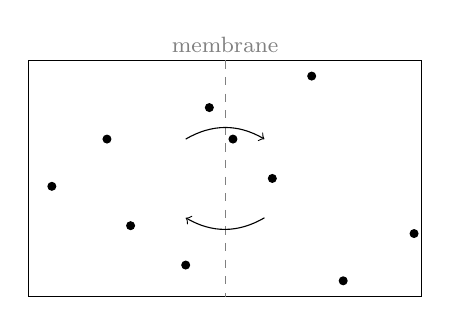
\begin{tikzpicture}
    \draw[draw=black] rectangle ++(5,3);
    \draw[gray,dashed](2.5,3)--(2.5,0);
    \node[circle,draw,fill=black,inner sep=1pt] at (1,2) {};
    \node[circle,draw,fill=black,inner sep=1pt] at (0.3,1.4) {};
    \node[circle,draw,fill=black,inner sep=1pt] at (2.3,2.4) {};
    \node[circle,draw,fill=black,inner sep=1pt] at (2,0.4) {};
    \node[circle,draw,fill=black,inner sep=1pt] at (1.3,0.9) {};

    \node[circle,draw,fill=black,inner sep=1pt] at (2.6,2) {};
    \node[circle,draw,fill=black,inner sep=1pt] at (4,0.2) {};
    \node[circle,draw,fill=black,inner sep=1pt] at (3.1,1.5) {};
    \node[circle,draw,fill=black,inner sep=1pt] at (4.9,0.8) {};
    \node[circle,draw,fill=black,inner sep=1pt] at (3.6,2.8) {};

    \node[gray] at(2.5, 3.2) {\footnotesize membrane};
    \draw [->] (2,2) to [bend left] (3,2);
    \draw [<-] (2,1) to [bend right] (3,1);
\end{tikzpicture}
		\end{figure}
	\end{minipage}\par
	The difference with respect to the previous example is that now the process is a spatially inhomogeneous (but time homogeneuos) RW on $S$ finite. \\
	Define 
	\begin{equation*}
		X^{(N)}(t):= \frac{Y^{(N)}_{\lfloor Nt \rfloor} - N}{\sqrt{N}}
	\end{equation*}
	which implies 
	\begin{equation*}
		Y^{(N)}= i \quad \implies \quad i=x \sqrt{N}+ N
	\end{equation*}
	when $X^{(N)}(t) = x$.\\
	Let's rewrite the probabilities in terms of the $x$:
	\begin{align*}
		p_{x} (\Delta X^{(N)}(t) &= \pm \frac{1}{\sqrt{N}})= \mathbb{P}(\Delta Y^{(N)}_{\lfloor t/h_N \rfloor}= \pm 1| i = x\sqrt{N}+N)   \\
		&= \frac{1}{2} \pm \frac{N - (x \sqrt{N} + N}{2 N} \\
		&= \frac{1}{2} \pm\frac{x}{2 \sqrt{N}}
	\end{align*}
	spatial inhomogeneity. \\
	As we can see, we got a result very similar to the previous one with $x$ in place of $\mu$. \\
	\begin{align*}
		\mathbb{E}(\Delta X^{(N)}(t)) &= \frac{1}{\sqrt{N}}(\frac{1}{2} - \frac{x}{2 \sqrt{N}}) - \frac{1}{\sqrt{N}}(\frac{1}{2} + \frac{x}{2 \sqrt{N}}) \\
		&= - \frac{x}{2N} - \frac{x}{2N} = -\frac{x}{N} \hspace{ 0.5 cm} (h_N = \frac{1}{N};  \ \mu (x) = -x)
	\end{align*}
	\begin{equation*}
		\mE_x[(\Delta X^{(N)}(t))^2] = \frac{1}{N}(\frac{1}{2}-{\cancel{\frac{x}{2\sqrt{N}}}}) + \frac{1}{N}(\frac{1}{2}+{\cancel{\frac{x}{2\sqrt{N}}}}) = \frac{1}{N}
	\end{equation*}
	So, again, $\sigma^2(x) \equiv 1$.
	It is immediate to verify that the moment of order $4$:
	\begin{equation*}
		\mE_x[(\Delta X^{(N)}(t))^4] =O(\frac{1}{N^2})= o (\frac{1}{N})= o (h_N)
	\end{equation*}
	which implies that 
	\begin{equation*}
		X^{(N)} \xrightarrow{d} X
	\end{equation*}
	such that 
	\begin{equation*}
		d X(t) = - X(t) dt + d B(t), \quad X(t) \in \mR
	\end{equation*}
	called \textbf{Ornstein-Uhlenbeck diffusion}, stationary with respect to 
	\begin{equation*}
		N(0,\frac{1}{2})
	\end{equation*}
	It has applications in math finance and in biology. 
	Mean reversion: when it is the positive it pushes back to zero and when it is negative the process is pushed up to return to the $0$ that is the long mean of the process.
	This is particular because is a process that is stationary (BM is not stationary and this property is useful in many application mathfinance, bioology). \\
	We sent by $N$, we rescale and we determine a transformation of the previous one. We plot it and we find its Gaussian distribution. \\
	It can be seen as a continuous-time analogue of AR(1).\\
	Discretize over $\Delta t$ interval to get 
	\begin{equation*}
		\underbracket{\Delta  X_k}_{X_{k+1}-X_{k}} = - X_k \Delta t + \sqrt{\Delta t} \cdot\varepsilon_k 
	\end{equation*}
	where 
	\begin{equation*}
		\varepsilon_k \stackrel{i.i.d}{\sim}
		\mathcal{N}(0,\frac{1}{2})
	\end{equation*}
	which implies that 
	\begin{align*}
		\mE(\Delta X_k) ) & = - X_k \Delta t \\
		\mV ar(\Delta X_k) &= \frac{\Delta t}{2}
	\end{align*}
	and we write
	\begin{equation*}
		X_{k+1} = X_k -X_k \Delta t + \sqrt{\Delta t}\epsilon_k=\underbrace{1-\Delta t}_{a}X_k + \underbrace{\sqrt{\Delta t}}_{b}\epsilon_k
	\end{equation*}
	\item \textbf{Branching Processes}
	Consider 
	\begin{equation*}
		Y^{(N)}_n \text{ a BP   } Y^{(N)}_n = \sum_{i=1}^{Y^{(N)}_{n-1}} Z_i^{(N)}
	\end{equation*}
	where $n$ refers to the step, while $N$ the parameterisation and \\
	$Z_i^{(N)} \stackrel{i.i.d.}{\sim}$  
	with mean $\mu^{(N)} \in \mR$ and variance $\sigma^2 > 0$. 
	\begin{equation*}
		\mE[Y_n^{(N)}|Y_{n-1}^{(N)}=y] = \mu^{(N)}y  \hspace{0.5 cm}\implies \mE_y[\Delta Y_n^{(N)}]= \mu^{(N)} y -y =y(\mu^{(N)}-1)
	\end{equation*}
	Now observe:
	\begin{equation*}
		\text{Var}_y(Y_n^{(N)})=\sigma^2 y
	\end{equation*}
	Define
	\begin{equation*}
		X^{(N)}:= \frac{Y^{(N)_{\lfloor Nt \rfloor}}}{N}    
	\end{equation*}
	which implies that 
	\begin{equation*}
		X^{(N)}(t) = x \implies y = N x
	\end{equation*}
	\begin{equation*}
		\mE_x[\Delta X^{(N)}(t)]=\frac{1}{N}\mE_y[\Delta Y^{(N)}_{\lfloor Nt \rfloor}]=\frac{1}{N}y(\mu^{(N)}-1)
	\end{equation*}
	\begin{align*}
		\mE_x [(\Delta X^{(N)}(t))^2] &= \var_x (\Delta X^{(N)}(t)) + (\mE_x[\Delta X^{(N)}(t)])^2 \\
		& = \frac{1}{N^2} \underbrace{\var_y (\Delta Y_n )}_{\var_y (Y_{n+1} )+0 } + \frac{1}{N^2} Y^2(\mu^{(N)}-1)^2 \\
		&= \frac{1}{N^2}\sigma^2 y + \frac{1}{N^2}y^2(\mu^{(N)}-1)^2 
	\end{align*}
	if we let $\mu^{(N)}$ be a perturbation of 1, i.e. $\mu^{(N)}= 1 \frac{m}{N}$ so that $\mu^{(N)}- 1=  \frac{m}{N}$, then
	\begin{equation*}
		\mE_x [\Delta X] = \frac{1}{N} y \frac{m}{N} = \frac{my}{N^2} = \frac{mx}{N}
	\end{equation*}
	since $y = Nx$
	\begin{equation*}
		\mE_x[(\Delta X)^2] = \frac{\sigma^2 x }{N} + \underbrace{\frac{1}{N^2} N^2 x^2 \frac{m^2}{N^2}}_{o(\frac{1}{N})}
	\end{equation*}
	$h_N= \frac{1}{N}$, $\mu (x)= mx $ and $\sigma^2 = x$. \\
	\begin{equation*}
		\implies \qquad X^{(N)} \xrightarrow{d} X \qquad \text{s.t.}
	\end{equation*}
	such that 
	\begin{equation*}
		d X(t) = m X(t) dt + \sigma \sqrt{X(t)} dB(t)
	\end{equation*}
	This process is called 
	\begin{itemize}
		\item \textbf{Cox-Ingersoll-Ross diffusion} in math finance
		\item \textbf{Continuous state Branching Process} in math biology
	\end{itemize} 
	So, if we touch $0$ we are going to stay there forever. This is the situation we gained talking about Markov Chains and extinction of a certain population: once reached, the population stays extinguished. \\
	$0$ is an \textit{absorbing state}. \\
	This reasoning has also a discretised counterpart. \\
	\item \textbf{Wright-Fisher processes}\\
	The transitions
	\begin{equation*}
		Y_{n+1}^{(N)}|Y_n=i \sim \text{Binom}(N,\frac{i}{N})
	\end{equation*}
	are space inhomogeneous and indexed by $N$.
	
	\begin{equation*}
		X^{(N)}(t) := \frac{Y^{(N)}_{\lfloor Nt\rfloor}}{N}
	\end{equation*}
	the percentage of type $0$. \\
	For brevity of notation, 
	\begin{equation*}
		Z_x := (X^{(N)}(t+\frac{1}{N})|X^{(N)}(t)=\underbrace{x}_{i/N})\sim\frac{1}{N}\text{Binom}(N,x)
	\end{equation*}
	Let's now comput the first two moments, starting with the first one:
	\begin{equation*}
		\mE_x[\Delta X^{(N)}(t)] = \mE(Zx) - x  =\frac{1}{N} N x = 0
	\end{equation*}
	and moving on to the second moment:
	\begin{align*}
		\mE_x[(\Delta X^{(N)}(t)^2] &= \text{Var}_x[\underbracket{\Delta X(t)}_{z_x-x}] + (\underbrace{\mE_x[\Delta X(t)]}_{0})^2 \\
		&= \frac{1}{N^2}Nx(1-x) = \underbrace{\frac{1}{N}}_{h_N} \underbrace{x(1-x)}_{\sigma^2 (x)}
	\end{align*}
	So 
	\begin{equation*}
		X^{(N)}\xrightarrow{d} X
	\end{equation*}
	such that 
	\begin{equation*}
		dX(t) = \sqrt{X(t) (1-X(t))} d B(t)
	\end{equation*}
	\begin{figure}
		\centering
		
\pgfmathsetseed{654}
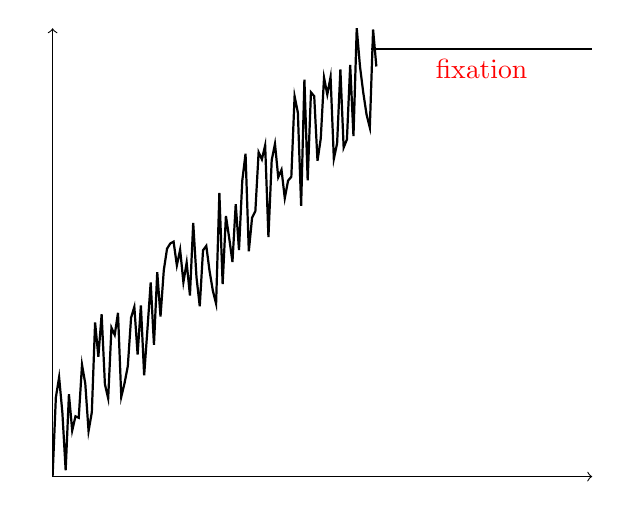
\begin{tikzpicture}
\begin{axis}[
                xlabel=\empty,
                x axis line style={->,opacity=100},
                ylabel=\empty,
                axis y line=left,
                %ymin=-0.6,ymax=2,
                xmin=0,xmax=50,
                y axis line style={->,opacity=100},
                ytick=\empty,
                xtick={85,170},
                xticklabels={$t_1$,$t_2$},
                axis x line*=bottom
                   ]     
    \addplot[black,domain = 0:30,
        samples = 100,
        thick] {2*x+10*rand};
    \addplot[black,thick]coordinates{(29.5,61.5)(50,61.5)}node[red,midway,below]{fixation};
\end{axis} %fashion
\end{tikzpicture}
	\end{figure}
	If all offspring are of type $0$, we are going to have always type $1$. Here it is the same way of thinking. \\
	Add mutations:
	\begin{equation*}
		Y_{n+1}| Y_n =i \sim Binom(N,p_i)
	\end{equation*}
	where $p_i = \alpha(1- \frac{i}{N}) + (1-\beta )\frac{i}{N}$ and, in turn, 
	\begin{align*}
		\alpha &= \mathbb{P}(1 \rightarrow 0) \\
		\beta &= \mP(0 \rightarrow 1)
	\end{align*}
	\begin{equation*}
		\Tilde{Z}_x := (X^{(N)}(t+\frac{1}{N})|X^{N}(t) = x) \sim \frac{1}{N} Binom(N, p_x)
	\end{equation*}
	where $x= \frac{i}{N}$ and $p_x = \alpha(\-x) + (1-\beta )x$. \\
	If we compute the increment of $X$, we have
	\[
	\mE_x[\Delta X(t)] = \mE_x[\Tilde{Z}_x] = x = \frac{1}{N} N p_x - x = \ldots = \frac{1}{N} \underbrace{[\alpha (1-x)-\beta x]}_{\mu(x)}
	\]
	
	% is there 2 in the [ ] at the end where it is underbraced?
	\begin{exercise}
	As exercise, show that 
	\begin{equation*}
		\mE_x[(\Delta X(t))^2]= \dots = \frac{1}{N}
		\underbrace{x(1-x)}_{\sigma^2(x)} + o (\frac{1}{N})
	\end{equation*}
	which implies that 
	\begin{equation*}
		X^{(N)} \xrightarrow{d} X
	\end{equation*}
	such that 
	\begin{equation*}
		d X(t) = [2(1-X(t)) - \beta X(t)]dt + \sqrt{ X(t) (1-X(t))} dB(t) = 0
	\end{equation*}
\end{exercise}
	if $X(t) = 0,1$. 
	\begin{itemize}
		\item at $X(t)=0$ we have $dX(t)= \alpha dt$
		\item at $X(t)=1$ we have $dX(t)= -\beta dt$
	\end{itemize}
	\begin{figure}[H]
		\centering
		
\pgfmathsetseed{654}
\begin{tikzpicture}
\begin{axis}[
                xlabel=\empty,
                x axis line style={-,opacity=100},
                ylabel=\empty,
                axis y line=left,
                ymin=-0,ymax=60,
                %xmin=0,xmax=50,
                y axis line style={-,opacity=0},
                ytick=\empty,
                xtick=\empty,
                %axis x line=bottom top
                   ]     
    \addplot[black,domain = 0:30,
        samples = 100,
        thick] {2*x+10*rand};
        \addplot[black,domain = 30:80,
        samples = 100,
        thick] {-1.5*x+10*rand+90};
        \addplot[black,domain = 80:240,
        samples = 250,
        thick,xshift={-20pt}] {1.4*(x+200)+10*rand-400};
        \draw [-{Stealth},very thick,red] (35,60) to (35,50);
        \draw [-{Stealth},very thick,red] (80,00) to (80,10);
\end{axis} %fashion
\node[] at (-0.5,5.7){1};
\node[] at (-0.5,0){0};
\end{tikzpicture}
	\end{figure}
	An application of the scaling limits is suggested by what we just wrote (?).\\
	\begin{itemize}
		\item we can avoid the computation of the conditional probability, which is very tricky.
		\item if the variance is small we cannot conclude that much. If it is too big, the process moves too much. So we study the limit diffusions under the problematic of rescaling. 
	\end{itemize}
	\end{enumerate}
	\begin{figure}[H]
		\centering
		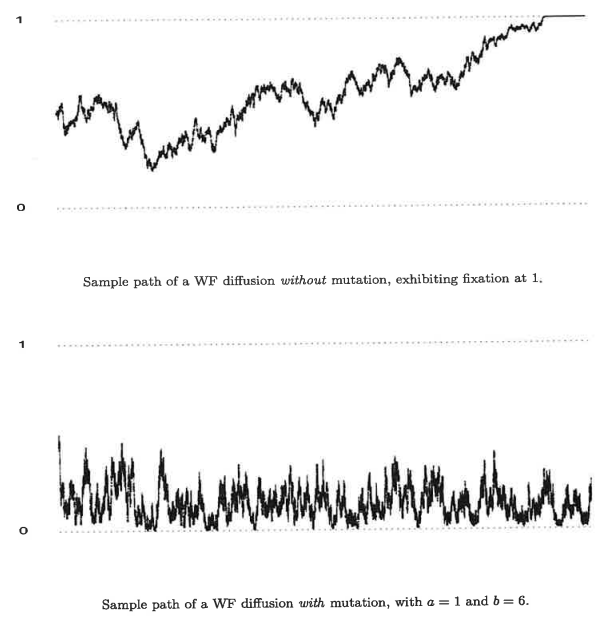
\includegraphics[width=0.7\linewidth]{drawings/samplepaths.png}
	\end{figure}
	\includepdf[pages=10,pagecommand={}]{drawings/Lec 16.pdf}
	A possible application of these concepts is in the approximation of stationary distributions:\par
	\begin{minipage}{0.5\textwidth}
		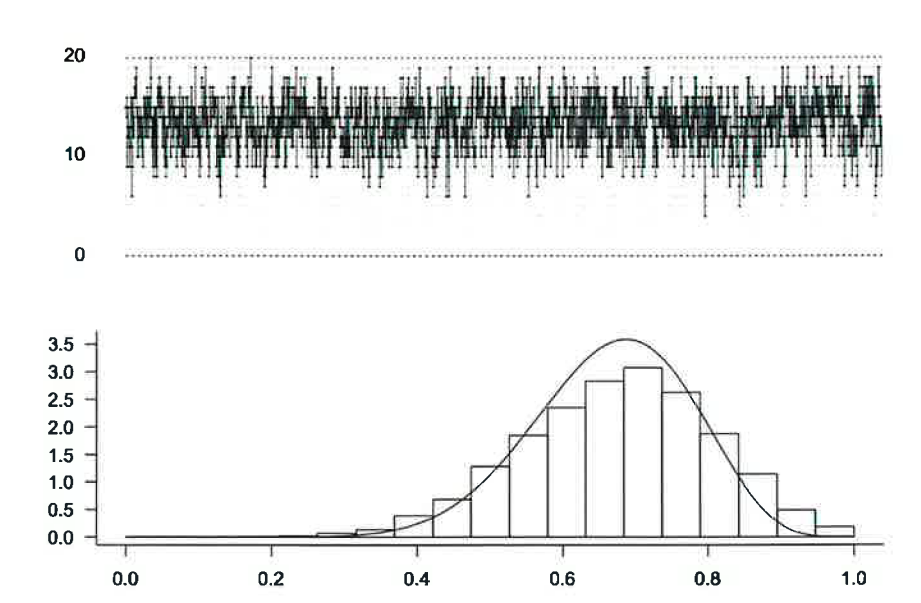
\includegraphics[width=1\linewidth]{drawings/approxstation.png}
	\end{minipage}\hfill
	\begin{minipage}{0.5\textwidth}
		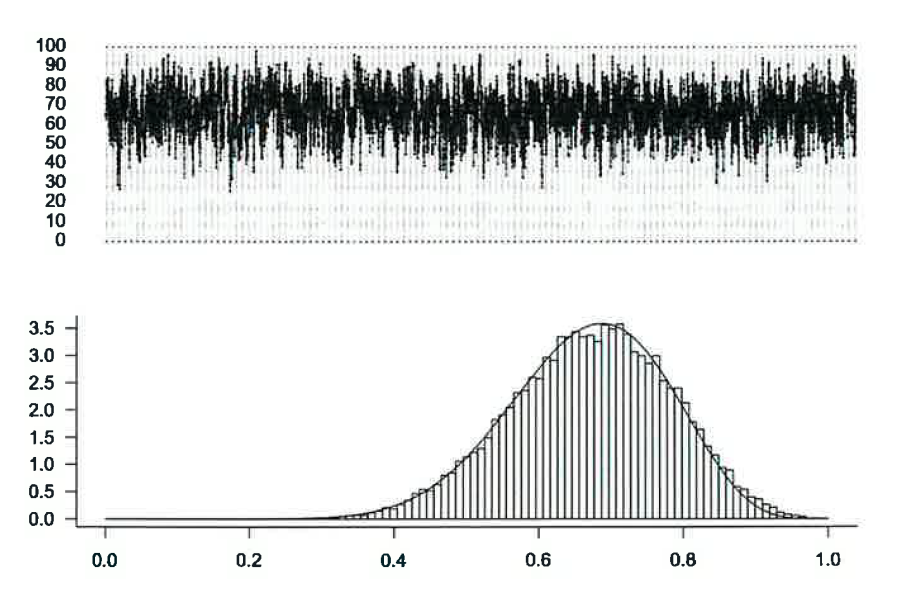
\includegraphics[width=1\linewidth]{drawings/approx2.png}
	\end{minipage}
	Another application may be the tuning of the variance in a Random Walk Metropolis-Hastings algorithm (trough the "Goldilocks" method) using scaling limits.
	\begin{figure}[H]
		\centering
		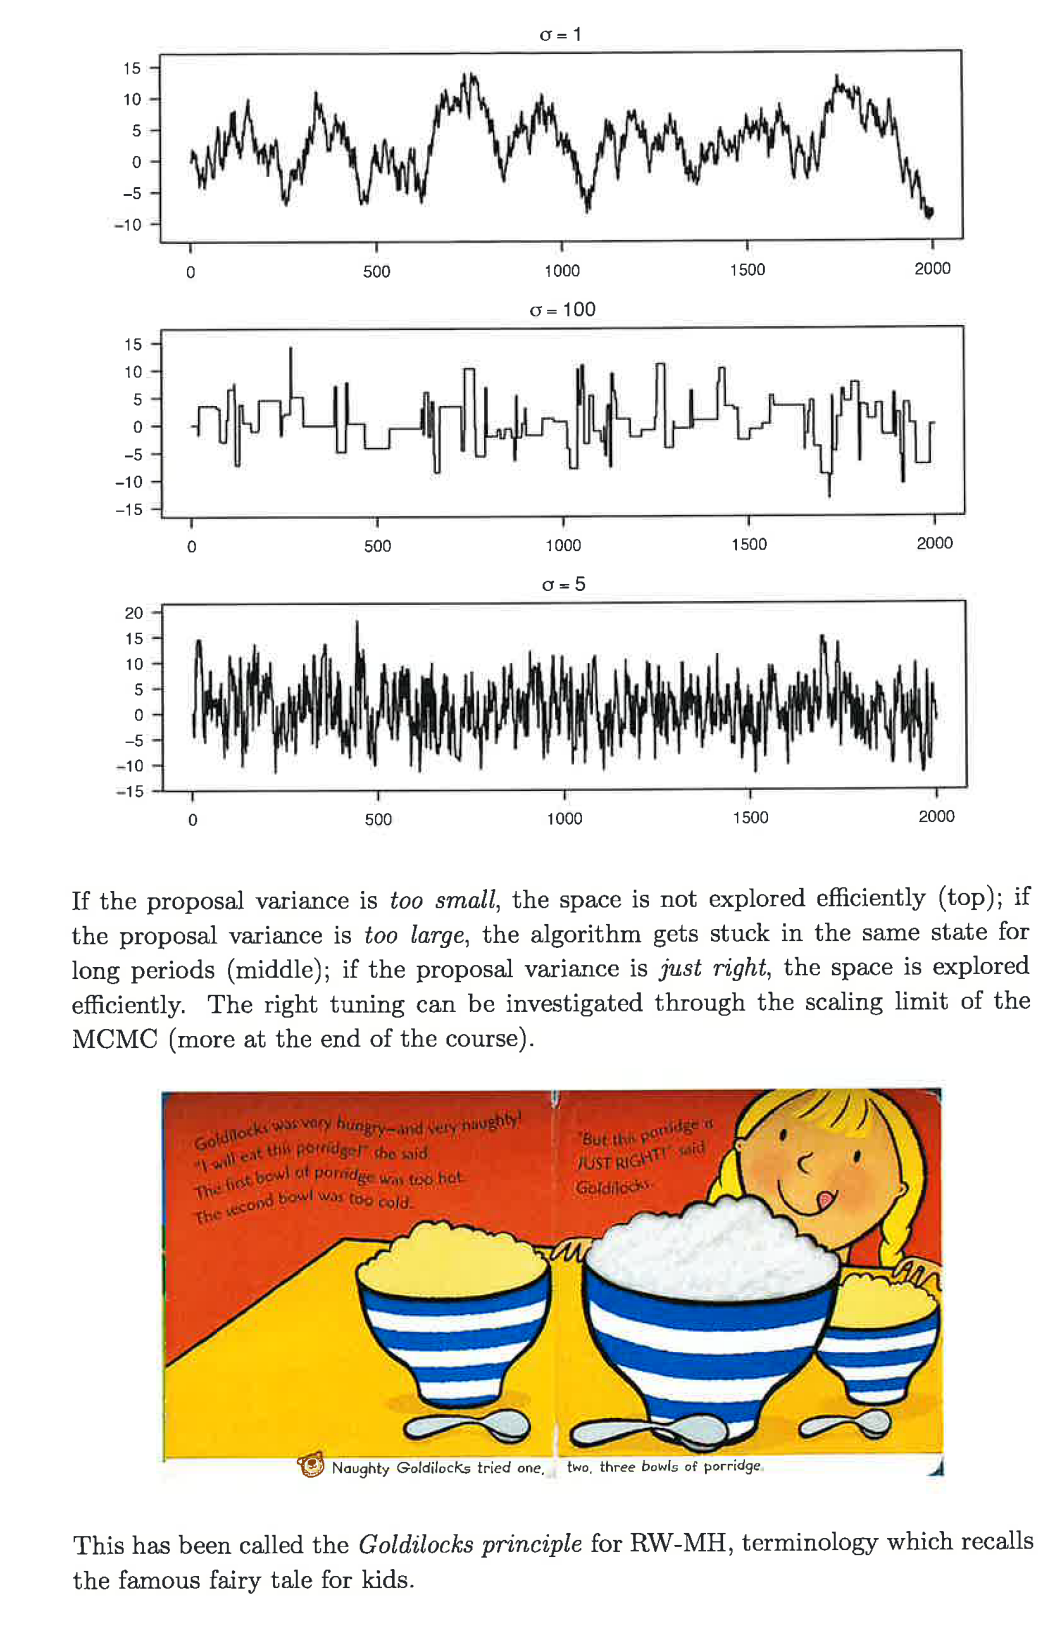
\includegraphics[width=0.67\linewidth]{drawings/goldilocks.png}
	\end{figure}
	We can also study different rescalings of a class of Random Walk Metropolis-Hastings algorithms and how to tune the variance of the proposal distribution accordingly:
	\begin{figure}[H]
		\centering
		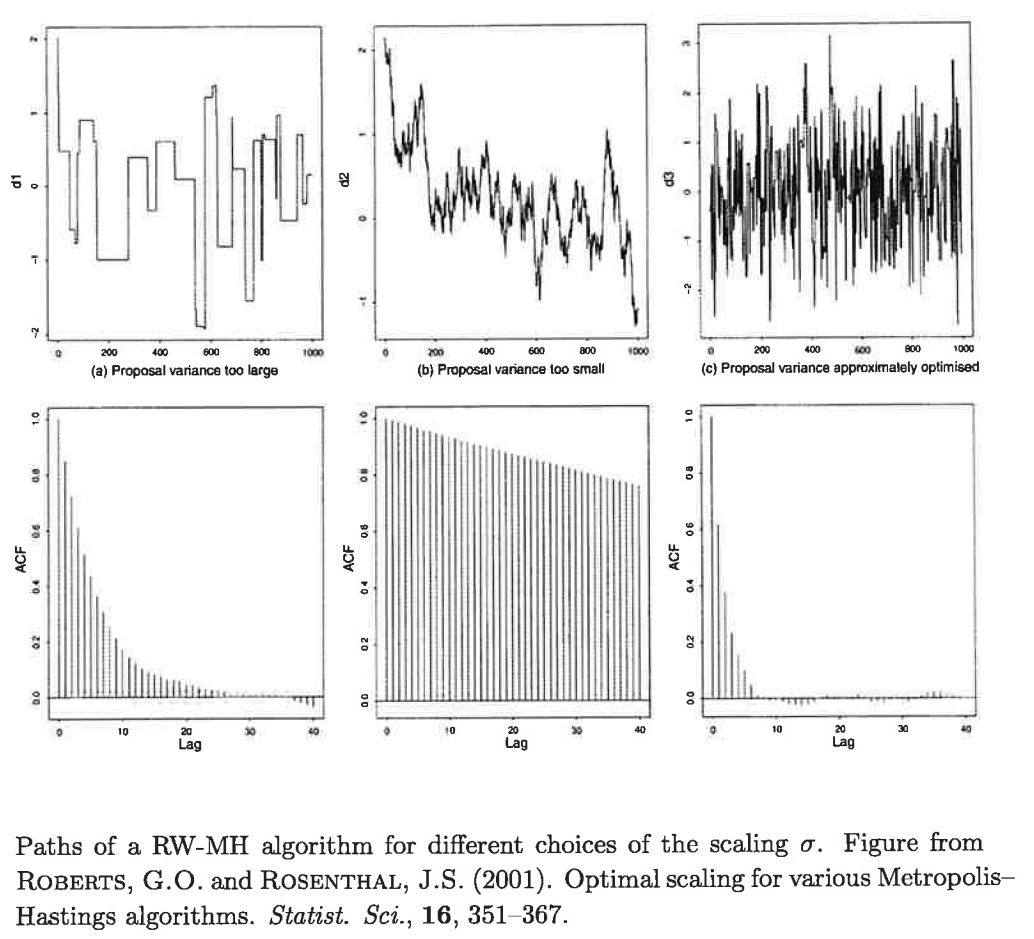
\includegraphics[width=1\linewidth]{drawings/variousrescalings.png}
	\end{figure}
	\section{L\'evy processes}
	\textbf{L\'evy processes} were introduced in the 1930's by Paul L\'evy and Bruno De Finetti, one of the fathers of Bayesian Statistics. These processes have important applications to mathematical finance, mathematical biology and nonparametric Bayesian inference.
	\begin{definition}
			A random variable $Y$ is said to be \textbf{infinitely divisible} (I.D.) if $\forall n \in \N$ there are $Y_i^{(n)}\; i.i.d.$ such that
		\[
		Y\stackrel{d}{=}Y_1^{(n)}+\ldots+Y_n^{(n)}
		\]
		i.e. $Y$ can be rewritten as sum of an arbitrary number $n$ of $i.i.d.$ random of variables.
	\end{definition}
	\begin{example}
		\begin{itemize}
			\item if \[
			Y\sim\text{Pois}(\lambda)\qquad:\qquad Y_i^{(n)}\stackrel{i.i.d.}{\sim}\text{Pois}\left(\frac{\lambda}{n}\right)
			\]
			by properties of the Poisson distribution, we know that
			\[\sum_{i=1}^{n}Y_i^{(n)}\sim \text{Pois}\left(\sum_{i=1}^{n}\frac{\lambda}{n}\right)=\text{Pois}(\lambda);\]
			\item If \[
			Y\sim\N(m,s^2)\qquad:\qquad Y_i^{(n)}\stackrel{i.i.d.}{\sim}N\left(\frac{m}{n},\frac{s^2}{n}\right)
			\]
			then $\sum_{i=1}^{n}Y_i^{(n)}\sim N(n,s^2)$;
			\item if \[
			Y\sim\Gamma(\alpha,\beta)\qquad:\qquad Y_i^{(n)}\stackrel{i.i.d.}{\sim}\Gamma\left(\frac{\alpha}{n},\beta\right)
			\]
			then $\sum_{i=1}^{n}Y_i^{(n)}\sim \Gamma(\alpha,\beta)$.
		\end{itemize}
	\end{example}
	A single way to establish I.D. is using $\ev{\exp^{iuk}}$. Take, for example, $Y\sim\text{Pois}(\lambda)$.
	\begin{align*}
		\ev{e^{iuY}}&=\sum_{k\geqslant0}\exp^{iuk}\lambda^k\frac{e^{-\lambda}}{k!}\\
		&=e^{-\lambda}\sum_{k\geqslant0}\frac{\left(\lambda\exp^{iu}\right)^k}{k!}\\
		&=e^{-\lambda}e^{\lambda e^{iu}}\\
		&=e^{-\lambda(1-e^{iu})}
	\end{align*}
	So $Y_i^{(n)}\stackrel{i.i.d.}{\sim}\text{Pois}(\frac{\lambda}{n})$. Consider now
	\begin{align*}
		\ev{\exp^{iu\sum_{i}^{n}Y_i^{(n)}}}&=\left[\exp^{-\frac{\lambda}{n}(1-\exp^{iu})}\right]^n\qquad \text{using }i.i.d.\text{ properties}\\
		&=e^{-\lambda(1-e^{iu})}.
	\end{align*}
	This suggests a strategy: we could define the \textbf{characteristic exponent} (c.e.) function of $Y$ to be:
	\[
	\psi(u)=-\log\ev{e^{iuY}}
	\]
	Then $Y$ is the I.D. if $\exists$ a random variable with c.e. $\psi^{(n)}$ such that:
	\[\psi(u)=n\psi^{(n)}(u).\]
	\begin{exercise}
		Check this fact for $N(m,s^2)$.
	\end{exercise}
	\begin{example}
		Consider $Y\sim\Gamma(\alpha,\beta)$. We have
		\[
		\ev(e^{iuY})=\frac{1}{\left(1-\frac{iu}{\beta}\right)^\alpha}=\left(\frac{1}{\left(1-\frac{iu}{\beta}\right)^\frac{\alpha}{n}}\right)^n
		\]
		which implies that 
		\[
		Y_i^{(n)}\stackrel{i.i.d.}{\sim}\Gamma(\frac{\alpha}{n},\beta)
		\]
	\end{example}
	\begin{definition}
		Let $N\sim$Poiss$(\lambda)$ and $Z_i\stackrel{i.i.d.}{\sim}F$ on $\R$ with $\mu_0$ mean at 0. The random variable
		\[Y\sum_{i=1}^{N}Z_i\qquad(Y=0 if N=0)\]
		is said to have \textbf{compound Poisson distribution}.
	\end{definition}
	Its characteristic function is:
	\begin{align*}
		\ev{e^{iu\sum_{i=1}^{N}Z_i}}&=\ev{\ev{e^{iu\sum_{i=1}^{k}Z_i}|N=k}}\\
		&=\sum_{k\geqslant0}\frac{\lambda^ke^{-\lambda}}{k!}\ev{e^{iu\sum_{i=1}^{k}Z_i}}\\
		&=\sum_{k\geqslant0}\frac{\lambda^ke^{-\lambda}}{k!}\bigl[\underbrace{\ev{e^{iuZ_1}}}_{\int_\R e^{iux}F(\dif x)}\bigr]^k\\
		&=\exp^{-\lambda}e^{\lambda\int_\R e^{iux}F(\dif x)}\\
		&=\exp^{-\lambda\int_\R(1-e^{iux})F(\dif x)}.
	\end{align*}
	Now,
	\begin{align*}
		\psi(u)&=\lambda\int_\R(1-e^{iux}F(\dif x))\begingroup\color{red}\cdot\frac{n}{n}\endgroup\\
		&=n\underbrace{\frac{\lambda}{n}\int_\R(1-e^{iux})F(\dif x)}_{\psi^{(n)}(u)}.
	\end{align*}
	So $Y$ is I.D. such that \[Y=\sum_{i=1}^{N}Z_i\stackrel{d}{=}\sum_{j=1}^{n}Y_j^{(n)}\]
	and we have
	\[
	Y_j^{(n)}=\sum_{i=1}^{N_j^{(n)}}Z-i,\qquad Z_i\stackrel{i.i.d}{\sim}F\text{ and }N_j^{(n)}\stackrel{i.i.d.}{\sim}\text{Poiss}\left(\frac{\lambda}{n}\right)
	\]
	Which is still a compounded Poisson with Poisson rate/mean $\frac{\lambda}{n}$.
	\begin{theorem}
		\textbf{L\'evy-Khintchine formula}. A random variable on $\R$ with c.e. $\psi(u)$ is I.D. if and only if there exists:
		\begin{itemize}
			\item $\mu \in \R$;
			\item $\sigma\geqslant 0$;
			\item a measure $\pi$ on $\R\setminus\{0\}$ satisfying:
			\[\int_\R(\underbracket{1\wedge x^2}_{\mathclap{\min\{1,x^2\}}})\pi(\dif x)<\infty\]
			such that, $\forall u\in\R$,
			\[\psi(u)=i\mu u +\frac{1}{2}\sigma^2 u^2+\int_\R\left(1-e^{iux}+iux\mathbbm{1}_{(|x|<1)}\right)\pi(\dif x).\]
		\end{itemize}
	\end{theorem}
	This characterizes I.D. distributions:
	\begin{itemize}
		\item $\pi$ is called \textbf{L\'evy intensity};
		\item $(\mu,\sigma,\pi)=(-m,s,0)$ is called \textbf{characteristic triplet}.
	\end{itemize}
	\begin{example}
		\begin{itemize}
			\item $(mu,\sigma,\pi)=(-m,s,0)$, i.e. $\pi\equiv0$:
			\[
			\psi(u)=-imu+\frac{1}{2}s^2u^2
			\]which is the c.e. of $N(m,s^2)$.
			\item $(\mu,\sigma,\pi)=(0,0,\lambda\delta_1)$:
			\begin{align*}
				\psi(u)&=\lambda\int_\R(1-e^{iux}+iux\underbracket{\mathbbm{1}_{(|x|<1)}}_{\mathclap{=0}})\delta_1(\dif x)\\
				&=\lambda\int_\R(1-e^{iux})\delta_1(\dif x)\\
				&=\lambda(1-e^{iu})
			\end{align*}which means that $Y\sim\text{Pois}(\lambda)$.
		\end{itemize}
	\end{example}
	The requirement \[\int_{\R}\min\{1,x^2\}\pi(\dif x)<\infty
	\]
	implies:
	\begin{itemize}
		\item $\int_{|x|\geqslant1}\pi(\dif x)<\infty$: the mean must be finite in both tails of $\pi$;
		\item $\int_{|x|\geqslant1}x^2\pi(\dif x)<\infty\implies$we can have $\pi\left((-1,1)\right)=\infty$ as long as $x^2\pi(\dif x)$ is integrable around 0.
	\end{itemize}
	For instance, $\pi(\dif x)\approx\frac{1}{x}\dif x$ around 0 is allowed.
	\begin{figure}[H]
		\centering
		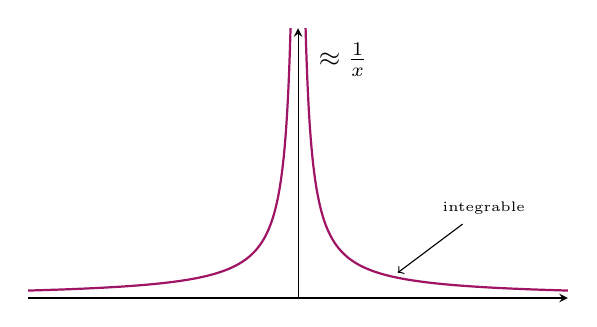
\begin{tikzpicture}
 \begin{axis}[
 	unit vector ratio*=1 1 1,
	axis lines = middle,
	ytick=\empty,
	xtick={0},
	xticklabel={0},
	scaled ticks = false,
	xmin = -6,
	xmax = 6,
	ymin = 0,
	ymax = 6,
	]
	\addplot[
	RedViolet, 
	thick, 
	domain = 0:20,
	samples=1000, 
	]
	{1/x};
	\addplot[
	RedViolet, 
	thick, 
	domain = 0:-20,
	samples=1000, 
	]
	{abs(1/x)};
	\node [anchor=west](source) at (axis cs:3,2) {\tiny integrable};
	\node (destination) at (axis cs:2,0.4){};
	\draw[->](source)--(destination);
	\node(lol) at(axis cs:1,5.3) {$\approx\frac{1}{x}$};
\end{axis}
\end{tikzpicture}
	\end{figure}
	\begin{definition}
			A L\'evy process on $\R$ is a continuous-time Càdlàg process $\{X(t),t\geqslant0\}$ such that:
		\begin{itemize}
			\item $X(0)=0$ a.s.;
			\item $X(s+t)-X(s)\stackrel{d}{=}X(u+t)-X(u)\qquad\forall s, u,t\geqslant0$: it has \sott{stationary increments};
			\item $X(s+t)-X(s)\independent\{X(u),u\leqslant s\}$: it has \sott{independent increments}.
		\end{itemize}
	\end{definition}
	\begin{example}
		Poisson process:
		\begin{itemize}
			\item $X(0)=0$ a.s.;
			\item $\underbracket{X(s+t)-X(s)}_{\mathclap{\independent s,X(s)}}\sim\text{Pois}(\lambda)$.
		\end{itemize}
		Brownian motion:
		\begin{itemize}
		\item $X(0)=0$ a.s.;
		\item $X(s+t)-X(s)\sim N(0,t)\independent s,X(s)$.
		\end{itemize}
	\end{example}
	\begin{definition}
		Let $N(t)$ be a rate $\lambda$ Poisson process and let $Y_i\stackrel{i.i.d.}{\sim}F$, independent of $N(t)$. Then
		\[X(t):=\sum_{i=1}^{N(t)}Y_i\qquad t\geqslant 0\] 
		is called \textbf{compound Poisson process}.
	\end{definition}
	\begin{exercise}
		Show that a CPP is also a L\'evy process and when $F=\delta_1$ it is a normal Poisson process.
	\end{exercise}
	\begin{figure}[H]
		\centering
		\begin{tikzpicture}%[scale=0.8]
	\begin{axis}[
		xlabel=\empty,
		x axis line style={->,opacity=100},
		ylabel=\empty,
		xmin=-1, xmax=100,
		ymin=-1, ymax=100,
		axis y line=left,
		y axis line style={->,opacity=100},
		ticks=none,
		axis x line*=bottom
		]
		\draw [RedViolet](0,0)--(30,0) node[circle,fill, pos=0,inner sep=2pt]{};
		\draw [RedViolet](30,60)--(50,60) node[circle,fill, pos=0,inner sep=2pt]{};
		\draw [RedViolet] (50,30)--(85,30) node[circle,fill, pos=0,inner sep=2pt]{};
		\draw [RedViolet] (85,80)--(100,80) node[circle,fill, pos=0,inner sep=2pt]{};
		\draw[dashed] (30,60)--(30,0);
		\draw[dashed] (50,60)--(50,30);
		\draw[dashed] (85,80)--(85,30);
		\begin{scope}[decoration=brace]
			\pgfdecorationsegmentamplitude=5pt
			\draw[decorate,black!80!black] (31,59)--(31,0) node[midway,right=\pgfdecorationsegmentamplitude,font=\tiny] {$Y_1$};
			\draw[decorate,black!80!black] (51,59)--(51,31) node[midway,right=\pgfdecorationsegmentamplitude,font=\tiny] {$Y_2$};
			\draw[decorate,black!80!black] (86,79)--(86,31) node[midway,right=\pgfdecorationsegmentamplitude,font=\tiny] {$Y_3$};
		\end{scope}
	\end{axis}
	\node[RedViolet,below right=0.1cm and 0.43cm, font=\tiny] (T) {Exp$(\lambda)$};
	\node[RedViolet,below right=0.1cm and 2.25cm, font=\tiny] (Te) {Exp$(\lambda)$};
\end{tikzpicture}
	\end{figure}
	\begin{exercise}
		Show that a finite sum of L\'evy processes is a L\'evy process.
	\end{exercise}
	\begin{example}
		$X(t)=\underbracket{X^{(1)}(t)}_{CP}+\underbracket{X^{(2)}(t)}_{BM}$
		\begin{figure}[H]
			\centering
			\documentclass{standalone}
\usepackage[framemethod=default]{mdframed}
\usepackage{tikz-cd}
\usepackage{tikz}
\usepackage[scr=rsfs]{mathalpha}
\usepackage[final]{pdfpages}
\usepackage{pgfplots,pgfplotstable}%per disegni
\usepgfplotslibrary{fillbetween}
\pgfplotsset{compat=1.16}
\usepackage{float}%per posizionamento disegni
\usetikzlibrary{shapes,patterns,arrows,positioning,calc,arrows.meta, bending, graphs, shadings,quotes,intersections,decorations}
\begin{document}

\pgfmathsetseed{654}
\begin{tikzpicture}
\begin{axis}[
  axis x line=center,
  axis y line=center,
  xtick=\empty,
  ytick=\empty,
  xlabel style={below right},
  ylabel style={above left},
  xmin=-10,
  xmax=160,
  ymin=-100,
  ymax=100]     
    \addplot[smooth,black,domain = 0:30.1,
        samples = 20,
        thick, name path=A] {(2*x-10)+7*rand};
        \addplot[smooth,black,domain = 29.9:80.1,
        samples =20,
        thick, name path=B] {(10*sin(8*(x+10))+10*rand+80};
        \addplot[smooth,black,domain = 79.9:150,
        samples = 25,
        thick,name path=C] {(-x+100)+10*rand};
    \path[name path=p1] (30,0)--(30,150);
    \path[name path=p2] (80,0)--(80,150);
    \fill [name intersections={of=A and p1}] (intersection-1) coordinate (a);
    \fill [name intersections={of=B and p1}] (intersection-1) coordinate (b);
    \fill [name intersections={of=B and p2}] (intersection-1) coordinate (c);
    \fill [name intersections={of=C and p2}] (intersection-1) coordinate (d);
    \draw[RedViolet,thick,dashed](a)--(b)node[midway,font=\tiny,right]{$Y_1$};
    \draw[RedViolet,thick,dashed](c)--(d)node[midway,font=\tiny,right]{$Y_2$};
\end{axis} %fashion
\end{tikzpicture}

\end{document}
		\end{figure}
		\begin{figure}[H]
			\centering
			\documentclass{standalone}
\usepackage{standtikz}
\begin{document}
\pgfmathsetseed{634}
\begin{tikzpicture}
\begin{axis}[
  axis x line=center,
  axis y line=center,
  xtick={0,15,30,45,135,150},
  xticklabels={$0$,$\frac{t}{n}$,$\frac{2t}{n}$,\empty,$\frac{(n-1)t}{n}$,$t$},
  ytick=\empty,
  xlabel style={below right},
  ylabel style={above left},
  xmin=-10,
  xmax=160,
  ymin=-10,
  ymax=100]     
    \addplot[smooth,black,domain = 0:150.1,
        samples = 30,
        thick, name path=A] {(0.6*x)-3+7*rand} node[pos=0.9,xshift=5pt,yshift=28pt,font=\scriptsize]{$X(t)$};
        \path (axis cs:0,0) 
        node [anchor=north west,yshift=-0.05cm] {0};
        \path[name path=tn](15,0)--(15,200);
        \path[name path=2tn](30,0)--(30,200);
        \path[name path=vuoto](45,0)--(45,200);
        \path[name path=nm1t](135,0)--(135,200);
        \path[name path=ciao](150,0)--(150,200);
        \fill[name intersections={of=A and tn}] (intersection-1) coordinate (a);
        \fill[name intersections={of=A and 2tn}] (intersection-1) coordinate (b);
        \fill[name intersections={of=A and vuoto}] (intersection-1) coordinate (c);
        \fill[name intersections={of=A and nm1t}] (intersection-1) coordinate (d);
        \fill[name intersections={of=A and ciao}] (intersection-1)coordinate (e);
        \draw[dotted,RedViolet!70!white,thick](15,0)--(a);
        \draw[dotted,RedViolet!70!white,thick](30,0)--(b);
        \draw[dotted,RedViolet!70!white,thick](45,0)--(c);
        \draw[dotted,RedViolet!70!white,thick](135,0)--(d);
        \draw[dotted,RedViolet!70!white,thick](150,0)--(e);
\end{axis} %fashion
\end{tikzpicture}

\end{document}
		\end{figure}
	\end{example}
	Let $X(t)$ be a L\'evy process and write:
	\begin{align*}
		X(t)&=\underbracket{X\left(\frac{t}{n}\right)-X(0)}_{\mathclap{\textcolor{RedViolet}{Y_1^{(n)}}}}+\underbracket{X\left(\frac{2t}{n}\right)-X\left(\frac{t}{n} \right) }_{\mathclap{\textcolor{RedViolet}{Y_2^{(n)}}}}+\ldots+\underbracket{X\left(t\right)-X\left(\frac{(n-1)t}{n} \right) }_{\mathclap{\textcolor{RedViolet}{Y_n^{(n)}}}}\\
		&\implies Y_i^{(n)}\stackrel{i.i.d.}{\sim}\qquad\text{from indepedence and stationarity of increments}\\
		&=\sum_{i=1}^{n}Y_i^{(n)}
	\end{align*}
	So $X(t)$ is I.D..\par
	Define 
	\[\psi_t(u):=\log\ev{e^{iuX(t)}}.\]
	as the c.e. of $X(t)$, from the sum:
	\[\text{if }t=m\in\N\qquad\begin{cases}
		\psi_m=n\psi_{\frac{m}{n}} &n\in\N\\
		\psi_m=m\psi_1&n=m
	\end{cases}\implies\psi_{\frac{m}{n}}=\frac{m}{n}\psi_1\]
	that is, $\forall t$ rational 
	\begin{equation*}
		\psi_t(u) = t \psi_1(u)
	\end{equation*}
	can be extended to $t \geqslant 0$. \\
	So
	\begin{equation*}
		\forall t \geqslant 0, \quad \psi_t(u) = t \psi_1(u)
	\end{equation*}
	So any L\'evy process is such that 
	\begin{equation*}
		\mE[e^{i u X(t)}] = e^{- t \psi_1(u)}
	\end{equation*}
	and so it is characterised by its characteristic exponent at $t=1$; therefore, the L\'evy-Khintchine formula provides a characterisation of L\'evy processes.\\
	\textbf{Example: Linear Brownian Motion}\\
	\begin{equation*}
		d X(t) = m dt + s dB(t)
	\end{equation*}
	$\implies$
	\begin{equation*}
		X(t) \sim N(mt, s^2 t)
	\end{equation*}
	$\implies$
	\begin{align*}
		\mE[e^{i u X(t)}] &= e^{i (mt) u - \frac{1}{2}(s^2 t) u^2}\\
		&= \exp\Bigg\{{\underbracket{-t\underbrace{\left[-imu + \frac{1}{2}s^2 u^2\right]}_{\psi_1(u)}}_{t \psi_1(u)}}\Bigg\}
	\end{align*}
	So at time $t = 1$, we find the triplet 
	\begin{equation*}
		(\mu, \sigma, \pi) = (-m, s,0)
	\end{equation*}
	This suggests:
	\begin{itemize}
		\item $\mu$ describes a constant drift with slope $ -\mu$
		\item $\sigma$ describes a Brownian component with diffusion coefficient $\sigma^2$. 
	\end{itemize}
	\begin{example}
		CP:
		\begin{equation*}
			X(t) = \sum_{i=1}^{N(t)} Z_i
		\end{equation*}
		with 
		\begin{equation*}
			N(t) \sim Po(\lambda t)
		\end{equation*}
		and 
		\begin{equation*}
			Z_i \stackrel{i.i.d.} \sim F
		\end{equation*}
		\begin{equation*}
			\psi_t(u) = t \psi_1(u)  
		\end{equation*}
		implies that at time $t=1$ we get a CP R.V.
		\begin{equation*}
			X(1) = \sum_{i=1}^{N(1)} Z_i
		\end{equation*}
		where $N(1) \sim Po(\lambda)$.
		This implies that 
		\begin{equation*}
			\psi_1(u) = \lambda \int_\mR (1-e^{iux}) F(\dif x)
		\end{equation*}
		We compute 
		\begin{align*}
			\psi_1(u) &= \lambda \int_\mR \left(1-e^{iux} + \textcolor{RedViolet}{iux \mathbbm{1}_{(|x| < 1)}} - \textcolor{Dandelion!70!black}{iux \mathbbm{1}_{(|x| < 1)}}\right)F(\dif x) \\
			&= \int_\mR \left(1-e^{iux} + iux\mathbbm{1}_{(|x| < 1)}\right)\color{RedViolet}\underbracket{\color{black}\lambda F(\dif x)}_{\color{RedViolet}\pi(\dif x)}\color{black} - iu\color{RedViolet}\underbracket{\color{black} \lambda \int_{-1}^1 x F(\dif x)}_{\color{RedViolet} -\mu}
		\end{align*}
		so the triplet is 
		\begin{equation*}
			\mu= -\lambda \int_{-1}^1 x F(\dif x), \quad \sigma = 0, \quad \pi = \lambda F
		\end{equation*}
		So:
		\begin{equation*}
			\lambda = \int_\mR \pi(\dif x)
		\end{equation*}
		called \textbf{total mass of $\pi$}, is the Poisson rate for jump arrivals. \\
	\end{example}
	\begin{remark}
		The L\'evy intensity of a CP has a finite total mass by construction!
	\end{remark}
	The normalized $\pi$ yields 
	\begin{equation*}
		F = \lambda^{-1} \pi
	\end{equation*}
	which gives the distribution of the jumps. \\
	\includepdf[page=14,pagecommand={}]{drawings/lec 17}
	We talked about 
	L\'evy processes, which are Markov processes with stationary and independent increments, characterized by the characteristic exponent at time $1$ through 
	\begin{equation*}
		\psi_t(u) = t \psi_1(u)
	\end{equation*}
	\subsection{Subclasses of L\'evy Processes}
	We introduced a different object, a compound Poisson process:
	\begin{equation*}
		X(t) = \sum_{i=1}^N(t) Z_i
	\end{equation*}
	with $Z_i \stackrel{i.i.d.} \sim F$ with no mass at 0. in particular
	$$N(t) \sim \text{Pois}(\lambda t)$$
	The characteristic exponent of a generic compound Poisson process is 
	\begin{equation*}
		\psi(u) = \lambda \int_\mR (1-e^{iux})F(\dif x)
	\end{equation*}
	\begin{remark}
		The $F$ is the distribution of the jump sizes and the lambda is the Poisson rate for jumps arrival. 
		$\lambda$ is the Poisson rate for jump arrivals
		\begin{equation*}
			\lambda = \int_\mR \pi(\dif x) < \infty
		\end{equation*}
		by construction. 
	\end{remark}
	We can add something to this.
	If we add a drift to the compound Poisson process, we obtain a L\'evy process with characteristic exponent given by the sum of the exponents:
	\begin{equation*}
		\lambda \int_\mR (1-e^{iux}) F(\dif x) - iub
	\end{equation*}
	where the drift is $bt$. \\
	\begin{exercise}
		Show the triplet is $(\mu, \sigma, \pi)$, where
		\begin{itemize}
			\item $\sigma = 0$
			\item $\pi = \lambda F$
			\item $\mu = - (b+\lambda \int_{-1}^1 x F(\dif x))$
		\end{itemize}
	\end{exercise}
	\begin{example}
		In the previous lecture we had shown that a random variable $Y \sim \Gamma(\alpha, \beta)$ is infinitely divisible with characteristic function 
		\begin{equation}
			\label{star1}
			\frac{1}{(1-\frac{iu}{\beta})^\alpha} \underbrace{=}_{\text{Frullani integral}}\exp\left\{-\int_0^\iy(1-e^{iux})\alpha x^{-1} e^{-\beta x}\dif x\right\}
		\end{equation}
		Now, clearly, the integral becomes the characteristic exponent for the random variable since we can see
		\begin{equation*}
			\int_0^\iy(1-e^{iux}\alpha x^{-1} e^{-\beta x} = \psi(u)
		\end{equation*}
		and 
		\begin{equation*}
			\alpha x^{-1} e^{-\beta x}\dif x = \pi(\dif x)
		\end{equation*}
		We can add and subtract $iux 1_{(|x|<1)}$ and therefore, similarly to CP process, we get 
		\begin{equation*}
			\psi(u) = \int_0^\iy (1-e^{iux} - iux 1_{(|x|<1)}\pi(\dif x) - iu \int_0^1x \pi(\dif x)
		\end{equation*}
		From this, we can read the L\'evy triplet 
		\begin{equation*}
			\mu = - \int_0^1x \pi(\dif x),  \quad \sigma = 0, \quad \pi(\dif x) = \alpha x^{-1} e^{-\beta x}\dif x
		\end{equation*}
	\end{example}
	We can define basing on this a L\'evy process, then we want to understand what does is mean in terms of trajectories. We have infinitive mass around 0.  \\
	We can use $\psi_t(u) = t \psi_1(u)$  to define a Gamma process as a L\'evy process with triplet as above, that is with exponent for $X(t)$ given by
	\begin{equation*}
		\psi_t(u) = \int_0^\infty (1-e^{iux})dt x^{-1}e^{\beta x}\dif x
	\end{equation*}
	Now we can work background and fine the increments of the process. \\
	So through \eqref{star1} we see that 
	\begin{equation*}
		X(t) \stackrel{d}= X(s+t) - X(s) \sim Ga(\alpha t, \beta)
	\end{equation*}
	We would like to know the behaviour in terms of trajectories. \\
	Note that:
	\begin{itemize}
		\begin{minipage}{0.5\textwidth}
			\item for $x \ra \infty, \pi(\dif x) \approx e^{-\beta x} $ is integrable \\$ \implies\pi((1,\infty)) < \infty$. 
		\end{minipage}
		\begin{minipage}{0.4\textwidth}
			\begin{figure}[H]
				\centering
				\documentclass{standalone}
\usepackage{standtikz}
\begin{document}
\begin{tikzpicture}[scale=0.6]
    \begin{axis}[
    xlabel=\empty,
                xtick={1},
                ytick=\empty,
                x axis line style={->,opacity=100},
                ylabel=\empty,
                xmin=0, xmax=5,
                ymin=0, ymax=2,
                axis y line=left,
                y axis line style={->,opacity=100},
                axis x line*=bottom
    ]\addplot[RedViolet, 
	thick, 
	domain = 1:20,
	samples=1000, 
 name path=iperboledemmerda
	]
	{1/x};
    \draw[black, dashed](1,0)--(1,1);
    \end{axis}
\end{tikzpicture}
\end{document}
			\end{figure}
		\end{minipage}\par
		\begin{minipage}{0.5\textwidth}
			\item for $x \ra 0^+$, $\pi(\dif x)  \approx \frac{1}{x}$ \\ $\implies \pi\left((0,1)\right)=\infty$: there is infinite mass in every neighbourhood of 0.
		\end{minipage}
		\begin{minipage}{0.4\textwidth}
			\begin{figure}[H]
				\centering
				\documentclass{standalone}
\usepackage{standtikz}
\begin{document}
\begin{tikzpicture}[scale=0.6]
    \begin{axis}[
    xlabel=\empty,
                xtick={1},
                ytick=\empty,
                x axis line style={->,opacity=100},
                ylabel=\empty,
                xmin=0, xmax=5,
                ymin=0, ymax=5,
                axis y line=left,
                y axis line style={->,opacity=100},
                axis x line*=bottom
    ]\addplot[RedViolet, 
	thick, 
	domain = 0:1,
	samples=100, 
 name path=iperboledemmerda
	]
	{1/x};
    \draw[black, dashed](1,0)--(1,1);
    \node[circle,anchor=west,font=\Large] at (2,2){$\infty$ mean};
    \draw[black,->,bend left](2,2) to [bend right](0.6,1.1);
    \end{axis}
\end{tikzpicture}
\end{document}
			\end{figure}
		\end{minipage}
	        The requirement in the L\'evy–Khintchine formula 
	\begin{equation*}
		\int_\mathbb{R} \min(1,x^2) \pi(\dif x) < \iy
	\end{equation*}
	
	is satisfied: around $0$ we have $\frac{x^2}{x}$. \\
	Technically we have something legitimate that we do not understand:
	since $\pi(\mathbb{R}_+)=\iy$ it is not a Compound Poisson.\\  
	\end{itemize}
	The Gamma process belongs to the following subclass of L\'evy processes.
	\begin{definition}
		 A \textbf{subordinator} is a L\'evy process with almost surely non-decreasing sample paths, hence with triplet:
		\begin{itemize}
			\item $\mu \leq 0$ (so we have a non-negative drift $-\mu$);
			\item $\sigma = 0$ that is, there is no Brownian component (indeed, it couldn't have this component because of its oscillations); %non so se ho capito bene il discorso. 
			\item $\pi((-\infty,0]) = 0$, (se we only select positive jumps). 
		\end{itemize}
	\end{definition}
	\begin{remark}
		The Gamma process is gonna be used a lot in Bayesian Statistics where we will use it to create appropriate prior distributions. 
	\end{remark}
	We want to understand path properties when $\pi$ has total mass. We write a generic characteristic exponent as follows
	\begin{equation*}
		\psi(u)  = \underbrace{i\mu u + \frac{1}{2}\sigma^2 u^2}_{\psi^{(1)}} + \underbrace{\int_{(-1,1)^c}(1-e^{iux})\pi(\dif x)}_{\psi^{(2)}} + \underbrace{\int_{(-1,1)}(1-e^{iux} + iux 1_{(|x|<1)})\pi(\dif x)}_{\psi^{(3)}}
	\end{equation*}
	$\psi^{(1)}$ is the exponent of a Brownian Motion
	\begin{equation*}
		d X^{(1)}(t) = - \mu dt + \sigma dB(t) 
	\end{equation*}
	\begin{itemize}
		\item $\psi^{(1)}:$ is a linear BM
		\item $\psi^{(2)}:$ outside $(-1,1)$ $\pi$ has finite mass so $\psi^{(2)}$ can be written as
		\begin{equation*}
			\lambda_0 \int_{(-1,1)^C} (1-e^{iux}) F_0(\dif x)
		\end{equation*}
		with $\lambda_0 := \pi((-1,1)^C)$ and $F_0 : = \lambda_0^{-1} \pi |_{(-1,1)^C}$.\\ 
		We look outside a neighborhood of zero and then we can normalize measure and therefore we can have a compound Poisson. \\
		So $\psi^{(2)}$ corresponds to a CP process with $\lambda_0$ Poisson rate and $F_0$ distribution for jumps of size $|x|\geq 1$.
		\item $\psi^{(3)}:$ we can distinguish two cases
		\begin{enumerate}
			\item $\pi((-1,1)) < \infty$
			\begin{equation*}
				\int_{-1}^{+1}(1-e^{iux} + iux)\underbracket{\pi(\dif x)}_{\mathclap{\substack{<\infty\text{: we can split}\\ \text{the integral}}}} = u x \pi(\dif x)\underbracket{\int_{-1}^{+1}(1-e^{iux})\pi(\dif x)}_{C.P.} + \underbracket{iu \int_{-1}^{+1} x \pi(\dif x)}_{\text{drift}}
			\end{equation*}
			\item $\pi((-1,1)) = \infty$
			Jumps arrive at infinite rate (the total mass is infinite) but we cannot normalize $\pi$ to get the jump distribution. 
			So, the condition 
			\begin{equation*}
				\int_R \min(1,x^2) \pi(\dif x)<\iy
			\end{equation*}
			implies:
			\begin{itemize}
				\item "big jumps" (size greater or equal than $1$) arrive at finite rate $\pi((-1,1)^C) < \infty$ hence they occur finitely often in every bounded interval. 
				\item If $\pi((-1,1)) = \infty$, "small jumps" arrive at infinite rate (precisely given by that mass), hence they occur infinitely often in every bounded interval. 
			\end{itemize}
		\end{enumerate}
		Even if it seems that the trajectories are somewhere flat, they are not: there are infinite small jumps. The Gamma process only increases by jumps. The trajectory are nowhere continuous. Such a process is said to have \textbf{infinite activity}.  
	\end{itemize} 
	\begin{definition}
		A measure $N$ on a $\sigma$-finite measure space $(\mathbb{X}, \mathcal{X}, \mu)$ is said to be a \textbf{Poisson random measure} (PRM) with mean intensity measure $\mu$ if for mutually disjoint sets $A_1,\dots,A_k \in\mathbb{X} $
		$$\mathcal{N}(A_i) \stackrel{i.i.d.} \sim  P_0(\mu(A_i))$$
	\end{definition} 
	\begin{example}
		$\mathbb{X} = \mathbb{R}_+ \times \mR$
		\begin{figure}[H]
			\centering
			\documentclass{standalone}
\usepackage{standtikz}
\begin{document}
\begin{tikzpicture}
\begin{axis}[
    xlabel=\empty,
                xtick=\empty,
                ytick=\empty,
                x axis line style={->,opacity=100},
                ylabel=\empty,
                xmin=-1, xmax=5,
                ymin=-1, ymax=2,
                axis y line=left,
                axis lines=middle,
                y axis line style={->,opacity=100}]
                \node[fill,circle,inner sep=1.5pt]at(1,1){};
                \node[fill,circle,inner sep=1.5pt]at(1.9,-0.5){};
                \node[fill,circle,inner sep=1.5pt]at(3,1.6){};
                \node[fill,circle,inner sep=1.5pt]at(4.1,0.6){};
                \node[fill,circle,inner sep=1.5pt]at(3.5,-0.9){};
                \node[fill,circle,inner sep=1.5pt]at(0.5,-0.7){};
                \node[fill,circle,inner sep=1.5pt]at(0.2,1.5){};
                \node[fill,circle,inner sep=1.5pt]at(4.7,1.2){};
                \node[fill,circle,inner sep=1.5pt]at(2.6,1.1){};
                \draw[RedViolet](2.4,0.4)--(2.4,1.7) node[midway,left]{$A$};
                \draw[RedViolet](2.4,0.4)--(4.9,0.4);
                \draw[RedViolet](4.9,0.4)--(4.9,1.7);
                \draw[RedViolet](4.9,1.7)--(2.4,1.7);
\end{axis}
\end{tikzpicture}
\end{document}
		\end{figure}
		$N(A) \stackrel{i.i.d.} \sim Po(\mu(A))$. \\
		If $A = [s,t] x [a,b] $, $\mu = \text{Lebesgue measure} \times \pi$
		\begin{equation*}
			\mu(A) = \lambda(t-s) \int_a^bF(\dif x)
		\end{equation*}
		where $\pi = \lambda F$. 
	\end{example}
	\begin{proposition}
		 Let $N$ be a PRM on $[0,\infty) \times \mR$ with mean intensity $\mu=Leb \times \pi$, with $\pi$ finite on $\mR$ such that $\pi(\{0\}) = 0$. \\
		For any Borel set $B \in \mathcal{B}(\mR)$ 
		\begin{equation*}
			X_B(t):= \int_0^t \int_B x N(ds,\dif x) 
		\end{equation*}
		is a compound Poisson process with rate $\lambda_B:= \pi(B)$ and jump distribution $F_B = \lambda_B^{-1} \pi|_B$. 
	\end{proposition}
	\begin{example}
		Assume that $B = \mR$, $\pi$ is finite. Then, we can show that 
		\begin{equation*}
			N = \sum_{i \geq 1}1_{(s_i,Z_i)}
		\end{equation*}
		which gives us the random point configuration.\\
		This yields that 
		\begin{equation*}
			\int_0^t \int_B x \sum_{i \geq 1}1_{(s_i,Z_i)} (ds,\dif x) = \bigotimes
		\end{equation*}
		What we are saying is: we take the s and accumulate the x and the x is the second coordinate z. Sum up the second coordinate, that is sum up the heights of everything.
		$$\bigotimes = \sum_{i\geq1} Z_i 1_{(s_i \in [0,t], Z_i \in B)}$$
		The PRM is a random object which gives us the properties of the sample paths.\\
		We sum points heigth of every point $(S_i, Z_i) \in [0,t] \times B$ (if $B = \mR$, we sum all jumps sizes/points heights in $(0,t]$). 
	\end{example}
	If we now let, for general $\pi$ (so in every $[0,t] \times [0,\varepsilon]$ there could be infinitely many points).
	\begin{align*}
		\varepsilon_m &= \frac{1}{x^m}, \quad m \geq 1\\
		B_m &= (-1, - \varepsilon_m] \cup [\varepsilon_m, 1)
	\end{align*}
	Set 
	\begin{equation*}
		X^{(\varepsilon,m)}(t) := \underbrace{\int_0^t\int_{B_m} x N(ds,\dif x)}_{\text{CP since} \pi(B_m)<\iy} - \underbrace{t \int_{B_m}x\pi(\dif x)}_{\text{drift}}
	\end{equation*}
	which has exponent 
	\begin{equation*}
		\psi^{(3,m)} = \int_{B_m}(1-e^{iux}) \pi(\dif x) + iu \int_{B_m} x \pi(\dif x)
	\end{equation*}
	informally, as $n \ra \infty$, we obtain the exponent we were looking for. \\
	\begin{equation*}
		\psi^{(3)}= \int_{|x|<1}(1-e^{iux} + iux)\pi(\dif x)
	\end{equation*}
	More formally:
	\begin{proposition}
		Let $X^{(3,m}$ be a L\'evy process with exponent $\psi^{(\varepsilon,m)}(CP + drift)$.\\
		As $m \ra \infty, X^{(3,m)} \stackrel{a.s.} \ra X^{(3)}$ uniformly over $[0,T]$, where $X^{(3)}$ is a L\'evy process with exponent $\psi^{(3)}$ and with at most countably-many discontinuities in every bounded interval.
	\end{proposition}
	If $C_n = [\frac{1}{2^n},\frac{1}{2^{n-1}}), B_m = \bigcup_{n = 1} ^ m C_n$:\\
	\begin{figure}[H]
		\centering
		\documentclass{standalone}
\usepackage{standtikz}
\begin{document}
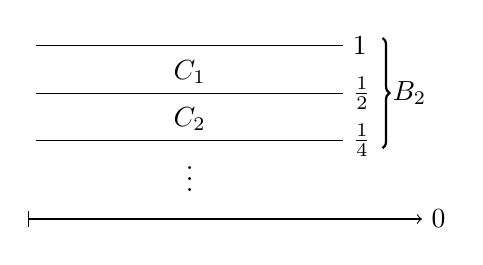
\begin{tikzpicture}[decoration=brace]
  \draw[|->,black] (0,0)--(5,0) node [anchor=west,pos=1]{0};
  \draw[black] (0.1,1)--(4,1) node [anchor=west,pos=1]{$\frac{1}{4}$}node[midway,anchor=south]{$C_2$} node[midway,anchor=north]{$\vdots$};
  \draw[black] (0.1,1.6)--(4,1.6) node [anchor=west,pos=1]{$\frac{1}{2}$} node[midway,anchor=south]{$C_1$};
  \draw[black] (0.1,2.2)--(4,2.2) node [anchor=west,pos=1]{1};
  \draw[black,decorate,thick] (4.5,2.3)--(4.5,0.9) node[anchor=west,midway]{$B_2$};
\end{tikzpicture}
\end{document}
	\end{figure}
	\begin{align*}
		\psi^{(\varepsilon,m)} &=\int_{B_m}(1-e^{iux}+iux)\pi(\dif x)=\\
		&=\sum_{n=1}^m[\lambda\underbracket{\int_{C_n}(1-e^{iux})F_n(\dif x)}_{C.P.}+ iu \lambda_n\underbracket{\int_{C_n}x F_n(\dif x)}_{\text{Drift}}]
	\end{align*}
	Hence the exponent of the process that converges to the limit process is given by a sum of cp processes whose jumps sizes are in disjoint intervals.
	\begin{theorem}
		\enf{L\'evy-Ito decomposition}. Let $(\mu, \sigma, \pi)$ satisfy the conditions of the L\'evy-Kinthchine formula. \\
		Any L\'evy process $X$ is the superposition of three intependent L\'evy processes, such that 
		\begin{equation*}
			X = X^{(1)} + X^{(2)} + X^{(3)}
		\end{equation*}
		where 
		\begin{enumerate}
			\item $X^{(1)}$ is a linear Brownian Motion $dX^{(1)} = \mu dt + \sigma dB(t)$
			\item $X^{(2)}$ is a CP with jumps low
			\begin{equation*}
				F_0:=\lambda_0^{(-1)} \pi |_{(-1,1)^C}
			\end{equation*}
			and rate 
			\begin{equation*}
				\lambda_0 := \pi((-1,1)^C)
			\end{equation*}
			\item $X^{(3)}$ is the sum of countably-many CP processes with drift and jumps in $(-1,1)$. 
		\end{enumerate}
	\end{theorem}
	\begin{exercise}
		Verify superposition of CP and parameterisation for the Gamma process. 
	\end{exercise}
	 So the Gamma process has no Brownian component, $\pi$ was on $mR_+$ and there was no drift. Hence, it is a process which there are infintely - many jumps in every small bounded interval. \\
	 \begin{figure}[H]
	 	\centering
	 	\begin{minipage}{.5\textwidth}
	 		\centering
	 		\includegraphics[page=11,scale=0.52,trim={4.3cm 7cm 4cm 5cm},clip]{drawings/Lec 18.pdf}
	 	\end{minipage}%
	 	\begin{minipage}{.5\textwidth}
	 		\centering
	 		\includegraphics[page=12,scale=0.52,trim={4.3cm 7cm 4cm 5cm},clip]{drawings/Lec 18.pdf}
	 	\end{minipage}
	 \end{figure}
	 \begin{figure}[H]
	 	\centering
	 	\begin{minipage}{.5\textwidth}
	 		\centering
	 		\includegraphics[page=13,scale=0.52,trim={4.3cm 7cm 4cm 5cm},clip]{drawings/Lec 18.pdf}
	 	\end{minipage}%
	 	\begin{minipage}{.5\textwidth}
	 		\centering
	 		\includegraphics[page=15,scale=0.52,trim={4.3cm 7cm 4cm 5cm},clip]{drawings/Lec 18.pdf}
	 	\end{minipage}
	 \end{figure}
	 \begin{figure}[H]
	 	\centering
	 	\includegraphics[page=14,scale=0.7,trim={4.3cm 12cm 4cm 5cm},clip]{drawings/Lec 18.pdf}
	 \end{figure}
\end{document}